\documentclass[11pt]{book}
\usepackage[paperwidth=17cm, paperheight=22.5cm, bottom=2.5cm, right=2.5cm]{geometry}
\usepackage{amssymb,amsmath,amsthm} %paquetes para símbolo matemáticos
\usepackage[spanish,mexico]{babel}
\usepackage[utf8]{inputenc} 
%Paquetes para escribir acentos y otros símbolos directamente
\usepackage{enumerate}
\usepackage{graphicx}
%\usepackage{subfig} %para poner subfiguras
\usepackage[pdftex,
            pdfauthor={Gian Carlo Di-Luvi Martínez},
            pdftitle={Diseno Bayesiano de experimentos para GLMs - Diluvi},
            pdfsubject={ESTADÍSTICA},
            pdfkeywords={PALABRAS CLAVE},
            pdfproducer={Latex con hyperref},
            pdfcreator={pdflatex}]{hyperref}
 
 
% Gian Carlo Diluvi's preamble ---------
\usepackage{amsthm}
\usepackage{amsmath}
\usepackage[nottoc]{tocbibind}
\usepackage{apacite} % Citar con APA
%\usepackage[numbers]{natbib}
\usepackage{natbib}
\AtBeginDocument{\renewcommand{\&}{y}} % Para citar como autor1 y autor2
%\usepackage{biblatex}
%\bibliography{bibliografia}
\usepackage{here}
\usepackage{float}
\usepackage{etoolbox}
\usepackage{url}
\usepackage{mathrsfs}
\usepackage{commath}
\usepackage[usenames, dvipsnames]{color}
\usepackage{multirow}
%\usepackage{subcaption}
\usepackage{dsfont} % Función indicadora

% Código --
\usepackage{listings}
	\lstset{frame = single,
    		literate={á}{{\'a}}1
        			 {ã}{{\~a}}1
        			 {é}{{\'e}}1
        			 {ó}{{\'o}}1
        			 {í}{{\'i}}1
        			 {ñ}{{\~n}}1
        			 {¡}{{!`}}1
        			 {¿}{{?`}}1
        			 {ú}{{\'u}}1
                     {Á}{{\'A}}1
                     {É}{{\'E}}1
                     {Í}{{\'I}}1
                     {Ó}{{\'O}}1
                     {Ú}{{\'U}}1
} 
\renewcommand{\lstlistingname}{Código}
\lstdefinestyle{R}{%
    %\captionsetup{labelformat=algocaption,labelsep=colon}
    mathescape=false,
    breaklines=true,
    frame=single,
    numbers=left, 
    numberstyle=\small,
    language=R,
    basicstyle=\scriptsize\ttfamily, 
    keywordstyle=\color{blue}\bf,
    xleftmargin=.04\textwidth,
    commentstyle=\color{OliveGreen},
    stringstyle=\color{OliveGreen},
    deletekeywords={mean, sd, start},
    morekeywords={TRUE, FALSE, seed}
}

\lstdefinestyle{thesis}{%
    %\captionsetup{labelformat=algocaption,labelsep=colon}
    mathescape=false,
    breaklines=true,
    frame=single,
    numbers=left, 
    numberstyle=\small,
    language=R,
    basicstyle=\scriptsize\ttfamily, 
    keywordstyle=\color{black}\bf,
    xleftmargin=.04\textwidth
}
%--

% Espaciado --
\renewcommand{\baselinestretch}{1.1}
%--

% Epígrafes --
\usepackage{epigraph}
%\epigraphfontsize{\small\itshape}
\setlength\epigraphwidth{0.8\textwidth}
\setlength\epigraphrule{0pt}
%--

% Apéndice
\usepackage[toc, page]{appendix}


\setlength{\parindent}{0pt}
\graphicspath{ {Images/} }

\usepackage{dsfont} %Para la función indicadora (mathds{1})

\usepackage{listings}   %Para introducir partes de código
    \lstset{language=R} %Para especificar qué lenguaje se usará
    
\usepackage{placeins} % Para utilizar \FloatBarrier


% Árboles de decisión
\usepackage{tikz}
\tikzset{
  treenode/.style = {shape=rectangle,
                     draw, align=center,
                     top color=white, bottom color=white},
  root/.style     = {treenode, font=\Large, bottom color=white},
  env/.style      = {treenode, font=\ttfamily\normalsize},
  dummy/.style    = {circle,draw}
}
\usetikzlibrary{arrows}


% Defs
\newcommand{\E}{\mathbb{E}}
\newcommand{\D}{\mathbb{D}}
\newcommand{\N}{\mathcal{N}}
\newcommand{\U}{\mathcal{U}}
\newcommand{\Exp}{\mathrm{exp}}
\newcommand{\V}{\mathrm{Var}}
\newcommand{\Binom}{\mathrm{Binom}}
\newcommand{\G}{\mathrm{Gamma}}
\newcommand{\Pois}{\mathrm{Poisson}}
%\newcommand{\lv}{\mathcal{l}}
\DeclareMathOperator*{\argmin}{arg\,min}
\DeclareMathOperator*{\argmax}{arg\,max} 
%\DeclareMathOperator{\argmin}{arg\,min}
%\DeclareMathOperator{\argmax}{arg\,max}

% End of GCD's preamble ----------------


\begin{document}

%------------------------------------------------------------------------------
%   COMANDOS PERSONALIZADOS
%------------------------------------------------------------------------------

%SI TU TESIS TIENE TEOREMAS Y DEMOSTRACIONES, PUEDES DESCOMENTAR Y USAR LOS SIGUIENTES COMANDOS 

%\renewcommand{\proofname}{Demostración}
%\providecommand{\norm}[1]{\lVert#1\rVert} %Provee el comando para producir una norma.
%\providecommand{\innp}[1]{\langle#1\rangle} 
%\newcommand{\seno}{\mathrm{sen}}
%\newcommand{\diff}{\mathrm{d}}

\newtheorem{theorem}{Teorema}[section] 
\newtheorem{corollary}[theorem]{Corolario}
\newtheorem{proposition}[theorem]{Proposición}
\newtheorem{lemma}[theorem]{Lema}

\theoremstyle{definition}
\newtheorem{definition}[theorem]{Definición}

%\theoremstyle{remark}
%\newtheorem{obs}[teo]{Observación}

%\allowdisplaybreaks


% Tabla en vez de cuadro
\renewcommand{\listtablename}{Índice de tablas} 
\renewcommand{\tablename}{Tabla}


%--------------------------------------------------------------------------------
%   PORTADA
%--------------------------------------------------------------------------------

\title{Diseno Bayesiano de experimentos para modelos lineales generalizados} 
%Con este nombre se guardará el proyecto en writeLaTex

\begin{titlepage}
\begin{center}

\textsc{\Large Instituto Tecnológico Autónomo de México}\\[4em]

%Figura
\begin{figure}[h]
\begin{center}

\includegraphics[width=10cm]{logo-ITAM-tesis.png}
\end{center}
\end{figure}

\vspace{2em}

\textsc{\huge \textbf{Diseño Bayesiano de experimentos para modelos lineales generalizados}}\\[2em]

\textsc{\large Tesis}\\[1em]

\textsc{que para obtener el título de}\\[1em]

\textsc{LICENCIADO EN MATEMÁTICAS APLICADAS}\\[1em]

\textsc{presenta}\\[1em]

\textsc{\Large GIAN CARLO DI-LUVI MARTÍNEZ}\\[1em]

\textsc{\large Asesor: DR. ERNESTO JUVENAL BARRIOS ZAMUDIO}

\end{center}

\vspace*{\fill}
\textsc{Ciudad de México \hspace*{\fill} 2018}

\end{titlepage}


%--------------------------------------------------------------------------------
%   DECLARACIÓN
%--------------------------------------------------------------------------------

\thispagestyle{empty}
\vspace*{\fill}
\begingroup
``Con fundamento en los artículos 21 y 27 de la Ley Federal del Derecho de Autor y como titular de los derechos moral y patrimonial de la obra titulada ``\textbf{Diseño Bayesiano de experimentos para modelos lineales generalizados}'', otorgo de manera gratuita y permanente al Instituto Tecnológico Autónomo de México y a la Biblioteca Raúl Bailléres Jr., la autorización para que fijen la obra en cualquier medio, incluido el electrónico, y la divulguen entre sus usuarios, profesores, estudiantes o terceras personas, sin que pueda percibir por tal divulgación una contraprestación''.

\centering

\hspace{3em}

\textsc{GIAN CARLO DI-LUVI MARTÍNEZ}

\vspace{5em}

\rule[1em]{20em}{0.5pt} % Línea para la fecha

\textsc{Fecha}
 
\vspace{8em}

\rule[1em]{20em}{0.5pt} % Línea para la firma

\textsc{Firma}

\endgroup
\vspace*{\fill}


%--------------------------------------------------------------------------------
%   Epígrafe
%--------------------------------------------------------------------------------


\frontmatter

\chapter*{}

\vspace{2cm}
\begin{flushright}
\textit{``Essentially, all models are wrong, but some are useful.''}\\
George E. P. Box
\end{flushright}



%--------------------------------------------------------------------------------
%   DEDICATORIA
%--------------------------------------------------------------------------------



\chapter*{Dedicatoria}


A Regina, Marcello, Regina, y Sarah.







%--------------------------------------------------------------------------------
%   AGRADECIMIENTOS
%--------------------------------------------------------------------------------

\chapter*{Agradecimientos}
%\markboth{AGRADECIMIENTOS23}{AGRADECIMIENTOS} % encabezado 

A Sarah, a falta de palabras suficientes, por todo. ``\textit{Your mind is my treasure, and if it were broken, it would be my treasure still.}''
\\

A mamá, porque sin tu apoyo incondicional nunca hubiera terminado esta aventura. \\


A mi familia, por siempre estar ahí para mí a lo largo de este trayecto. \\


A mi asesor, Ernesto Barrios, por guiarme en este camino e impulsarme a dar lo mejor de mí. \\

A mis sinodales, Manuel Mendoza, Luis Enrique Nieto y Gabriel Nuñez, por su tiempo, paciencia e interés. Sin ellos este trabajo no se hubiera completado. \\

A todos los profesores que compartieron sus conocimientos conmigo. Particularmente a Claudia Gómez, Manuel Mendoza, Ernesto Barrios, Vladimir Caetano, César Luis García, Marcela González, Guillermo Grabinsky, \newline Ernesto Pérez Chavela y Julia Sierra. \\


A la Bandera y a ($\varepsilon$ -- $\delta$). \\




%--------------------------------------------------------------------------------
%   TABLA DE CONTENIDOS
%--------------------------------------------------------------------------------

\tableofcontents


%\newpage

%\listoffigures

%\listoftables


%-------------------------------------------------------------------------------
%   TESIS
%-------------------------------------------------------------------------------

\mainmatter %empieza la numeración de las páginas
\pagestyle{headings}

%  Incluye los capítulos en el folder de capítulos


\chapter{Introducción} \label{chapter:intro}


\epigraph{\textit{Statistics is the grammar of science.}}{--- Karl Pearson}


La idea de que un estadístico es aquel a quien se le proporcionan datos para que los analice no podría estar más lejos de la realidad. Para que un estudio se lleve a cabo satisfactoriamente un estadístico debe estar involucrado desde antes de la recolección de los datos. Más aún, el trabajo del estadístico no termina con la conclusión del estudio. La investigación e innovación científica no es estática ni aislada, sino un proceso de autocorrección en el cual la experiencia previa guía y sugiere el camino a seguir \citep{box_liu_helicopter}. \\


El diseño de experimentos se refiere a la selección de todos los aspectos relevantes de un experimento y se realiza antes de la recolección de los datos. Debido a esto el paradigma Bayesiano resulta idóneo, ya que ofrece una manera de incorporar conocimientos previos al análisis \citep{bernardo_smith,notas_bayes_egp,notas_bayes}. Sin embargo, una de las desventajas de utilizar el enfoque Bayesiano es la latente complejidad computacional \citep{casella_george,geman_y_geman}. En el caso del diseño de experimentos ésta se traduce en la dificultad de evaluar funciones de pérdida sofisticadas que engloben los objetivos del experimento, así como integrales de dimensión sumamente alta \citep{Woods_etal}. \\


\cite{chaloner_verdinelli_doe} publicaron un artículo de revisión que ha servido como punto de referencia para el diseño Bayesiano de experimentos. Sin embargo durante un tiempo hubo un progreso práctico poco sustancial en este respecto, logrando encontrar soluciones solamente a problemas particulares. No obstante los últimos años han visto el surgimiento de algoritmos complejos que pretenden atacar estos problemas y mantener una eficiencia computacional tolerable. Hoy en día el método de \textit{Intercambio Aproximado de Coordenadas} (ACE por sus siglas en inglés) de \cite{Woods_ACE} se postula como la opción más efectiva para resolver problemas de diseño Bayesiano de experimentos, logrando encontrar diseños óptimos para una variedad de modelos y con la opción de personalizar la función de pérdida. Sin embargo su eficiencia depende altamente del número de ensayos y de la función de pérdida empleada. Más aún, su implementación no es trivial, lo que lo hace poco accesible para el público en general. \\ 




El diseño Bayesiano de experimentos generalmente aprovecha modelos populares y conocidos, como los modelos lineales generalizados \citep{nelder_wedderburn}. Estos son de particular interés porque permiten modelar una gran variedad de fenómenos, pero a la vez han sido estudiados con detalle \citep{glm_bayesian_view, nelder_glm, montgomery_glm}. El método ACE es más sencillo de implementar si se utiliza en conjunto con este tipo de modelos, lo que se traduce en un menor costo computacional, particularmente si se utilizan las funciones de pérdida que éste ya incluye. \\




Hoy en día disciplinas como la ingeniería, la medicina, y las ciencias sociales realizan experimentos estadísticamente diseñados \citep{fisher_doe, Woods_etal_2006}. Por lo tanto avances en la literatura sobre diseño experimental se traducen en una mayor variedad de diseños al alcance de más investigadores, incrementando la validez y reproducibilidad de los estudios científicos. Es por ello que impulsar la investigación sobre diseño de experimentos es imperativo, más aún considerando que siguen existiendo multiplicidad de complicaciones prácticas que restringen las opciones disponibles al diseñar un experimento. \\ 



El propósito de esta tesis es doble. Por un lado se desarrollarán los elementos teóricos detrás del diseño Bayesiano de experimentos. Esto es importante porque la gran mayoría de la literatura al respecto supone que el lector tiene conocimientos avanzados sobre diseño experimental y Estadística Bayesiana. Por lo mismo es difícil encontrar fuentes que contengan una revisión razonablemente completa del tema en cuestión. Más aún, se supondrá que el propósito último es modelar la relación entre algunas de las covariables del experimento y la variable respuesta mediante un modelo lineal generalizado. \\



Por otro lado se implementará el método ACE para resolver desde un enfoque Bayesiano dos problemas de diseño experimental, con el objetivo de constatar la eficacia de dicho algoritmo. En particular se replicarán dos de los resultados de \cite{Woods_etal}, los cuales suponen que la relación entre las covariables y la respuesta se describe mediante un modelo lineal generalizado. En ambos ejemplos se emplearán tanto las distribuciones iniciales propuestas por los autores como distribuciones diferentes, y además en el segundo experimento se utilizará también una función de pérdida distinta.




\section{Estructura de la tesis}


En el Capítulo \ref{chapter:bayesiana} se plantean los fundamentos de la Teoría de la Decisión que dan lugar a la Estadística Bayesiana. Para ello se discuten las limitaciones del enfoque clásico o frecuentista, se habla de problemas de decisión, y se discute su solución. Además se habla de la importancia del Teorema de Bayes, así como de la Estadística Bayesiana en la práctica. También se discute la complejidad computacional inherente al cálculo de la distribución final, y en el Apéndice \ref{chapter:appendixBayesiana} se muestran algunos de los métodos computacionales más populares para sobrepasar dicha dificultad. \\



En el Capítulo \ref{chapter:glms} se derivan los modelos lineales generalizados desde la perspectiva de componentes sistemática y aleatoria. Se hace particular énfasis en los modelos de regresión lineal, logística, y Poisson, los cuales se estudian a detalle 
en el mismo capítulo. Se discute también la estimación de los parámetros desde la perspectiva Bayesiana, particularmente para el caso de regresión lineal. \\

%En el Apéndice \ref{chapter:appendixGLMs}) se discute otro modelo lineal generalizado popular.  \\



En el Capítulo \ref{chapter:design} se formula el problema de encontrar un diseño óptimo como uno de decisión utilizando las herramientas del Capítulo \ref{chapter:bayesiana}. Así pues, se deduce la solución genérica de cualquier problema de diseño experimental y se mencionan las dificultades prácticas de encontrar dicha solución. También se discute sobre la importancia de la función de pérdida o utilidad, además de que se revisan las elecciones más populares en la literatura. Finalmente se revisa con detalle el método ACE de \cite{Woods_ACE}.\\



En el Capítulo \ref{chapter:doe_para_glms} se reproducen dos ejemplos de diseño Bayesiano de experimentos para modelos lineales generalizados tomados de \cite{Woods_etal}. El primero supone un modelo de regresión logística y el segundo uno de regresión Poisson. Se utilizarán funciones iniciales para los parámetros diferentes a las propuestas por los autores para resaltar la importancia de éstas, y además para el segundo caso se utilizará una función de pérdida diferente también. El código utilizado para este capítulo se incluye en el Apéndice \ref{chapter:appendixCode}. \\




En el Capítulo \ref{chapter:conclusiones} se da un resumen global de la tesis y se discuten los principales hallazgos, particularmente los referentes al Capítulo \ref{chapter:doe_para_glms}. Además se comentan las principales dificultades de la implementación del método ACE, así como sugerencias para posibles investigaciones futuras. \\

\newpage





\chapter[Estadística Bayesiana]{Teoría de la Decisión y Estadística Bayesiana} \label{chapter:bayesiana}

\epigraph{\textit{Bayesian Statistics offers a rationalist theory of personalistic beliefs in contexts of uncertainty, with the central aim of characterising how an individual should act in order to avoid certain kinds of undesirable behavioural inconsistencies.}}{--- Bernardo y Smith, \textit{Bayesian Theory} (2000)}


Aunque no se ha llegado a un consenso sobre una definición general de la Estadística, para propósitos de esta tesis ésta se definirá como \textit{un conjunto de técnicas cuyo propósito es describir fenómenos que se manifiestan a través de datos que presentan variabilidad} \citep{notas_bayes}. Esta definición resalta el ámbito de estudio (datos que presentan variabilidad) y el propósito (describir) de la Estadística. \\


Si bien el razonamiento y estudio de la Estadística se remonta al Siglo XVII,\footnote{Siglo en el que se comenzó a desarrollar la Teoría de la Probabilidad. La Estadística contemporánea no se desarrolló sino hasta el Siglo XIX.} no fue sino hasta el Siglo XX que ésta se formalizó (o, quizás mejor dicho, se ``matematizó'') gracias a las contribuciones de varios personajes, entre los cuales destacan Karl Pearson (1857-1936), Ronald Fisher (1890-1962) y Jerzy Neyman (1894-1981), entre muchos otros. Fue en estos años cuando los académicos de la época decidieron tratar de encontrar soluciones que tuvieran fundamentos matemáticos sólidos a los problemas que comúnmente se enfrentaban en la Estadística. El resultado de esta hazaña es lo que hoy se conoce como \textit{Estadística Matemática}; ésta surge como una serie de métodos o procedimientos que permiten resolver problemas como el de estimación puntual, estimación por regiones, pronósticos puntuales y por regiones, y contraste de hipótesis. A pesar de que la Estadística Matemática resultó ser (y sigue siendo) sumamente útil, algunos problemas comenzaron a surgir en los siguientes años; principalmente:

\begin{enumerate}
\item La Estadística Matemática no es una teoría, entendida en el sentido axiomático. No hay una serie de postulados de donde se puedan deducir simultáneamente todos los métodos que la conforman.\footnote{Esto contrasta fuertemente con la Teoría de la Probabilidad, que tiene como postulados a los axiomas de \cite{kolmogorov}.}
\item Como consecuencia de 1. pueden existir inconsistencias entre métodos. Algunas soluciones a un problema pueden no tener sentido, o incluso pueden contradecir otras soluciones.
\end{enumerate}

En años posteriores al desarrollo de la Estadística Matemática algunos estadísticos de la época trataron de solucionar estos problemas. Hay dos vertientes generales que logran este objetivo y desembocan en la Estadística Bayesiana: los teoremas de representación de Bruno de Finetti y la Teoría de la Decisión. En esta tesis se abordará la vertiente de la Teoría de la Decisión. El problema de diseño de experimentos (que se discute en el Capítulo \ref{chapter:design}) se trata también desde esta perspectiva. \\

El propósito de este capítulo es explicar los fundamentos de la Teoría de la Decisión y de la Teoría de la Inferencia Bayesiana necesarios para producir inferencia en el caso de los modelos lineales generalizados y para tratar el diseño de experimentos. Cabe mencionar que este capítulo no pretende desarrollar de manera profunda la Teoría de la Decisión; tampoco tiene como objetivo deducir la relación entre ésta y la Estadística Bayesiana más allá de lo necesario para su aplicación en capítulos subsecuentes. Si el lector está interesado en estos temas se le invita a consultar la bibliografía recomendada; en particular, ver \citep{bernardo_smith, mendoza_pena, notas_bayes}.


\section{Problemas de decisión}

Para el ser humano siempre ha sido de interés estudiar el proceso de toma de decisiones. Como \cite{mendoza_pena} mencionan, en la literatura generalmente hay dos formas de abordar este tema: una descriptiva y una normativa. La descriptiva pretende explicar cómo los agentes verdaderamente toman decisiones, y la normativa explica cómo \textit{deberían} tomarlas para satisfacer algún o algunos criterios previamente establecidos. Esta tesis se centrará en una Teoría de la Decisión normativa.\\

Un problema de decisión se refiere a la situación en la que un \textit{tomador de decisiones} debe seleccionar una, y solo una, opción de un conjunto de posibles decisiones, $\D$. Desde luego que esta decisión debe ser óptima en algún sentido. En particular las decisiones deben estar relacionadas con sus respectivas consecuencias, y es con éstas que la optimalidad de la decisión debe ser juzgada. De hecho debe existir una relación de orden $\succ$ en el conjunto de consecuencias, $\mathbb{C}$, que permita determinar cuál de éstas es más preferible. La terna $( \D, \mathbb{C}, \succ )$ se conoce como \textit{problema de decisión con certeza} cuando a cada decisión en $\D$ se le asocia, sin incertidumbre, una consecuencia en $\mathbb{C}$. Sin embargo, en la práctica cuando una decisión ha sido seleccionada generalmente hay una serie de consecuencias que pueden ocurrir; más aún, no hay certeza sobre cuál consecuencia ocurrirá. Así pues a cada decisión se le asocia también un conjunto de eventos inciertos relevantes, cada uno de los cuales está a su vez asociado con una consecuencia. Aquí ya estamos hablando de un \textit{problema de decisión en ambiente de incertidumbre}, cuya definición se enuncia a continuación para futura referencia. \\

\begin{definition}[Problema de Decisión] \label{def:decision_problem}
Un problema de decisión en ambiente de incertidumbre es una cuarteta $( \D, \mathbb{E}, \mathbb{C}, \succ )$, donde:
\begin{enumerate}
\item $\D = \{ d_1, d_2, ..., d_k \}$ es el conjunto de posibles decisiones.
\item $\mathbb{E}$ es el conjunto de eventos inciertos relevantes, de tal forma que a cada decisión $d_i$ le corresponde un conjunto de eventos inciertos relevantes
$\mathbb{E}_i = \{E_{i1}, E_{i2}, ..., E_{i n_i} \} \subset \mathbb{E}$, donde $E_{ij} \cap E_{ij'} = \emptyset$ para $j \neq j'$.
\item $\mathbb{C}$ es el conjunto de consecuencias, de tal forma que a cada evento incierto relevante $E_{ij}$ le corresponda unívocamente una consecuencia $c_{ij} \in \mathbb{C}$.
\item $\succ$ es una relación de orden en $\mathbb{C}$ que determina, dadas dos consecuencias, cuál es más preferible (o si son igualmente preferibles) para el tomador de decisiones.
\end{enumerate}
\end{definition}

Los eventos inciertos relevantes deben considerar todas las consecuencias, de manera que, para cualquier $i$,
\begin{equation*}
\bigcup_{j} E_{ij} = \Omega,
\end{equation*}
donde $\Omega$ es el evento seguro.\footnote{El evento seguro es aquel que ocurre con probabilidad 1, y se refiere al hecho de que los eventos inciertos relevantes asociados a una decisión deben considerar todas las posibilidades a ocurrir.} En otras palabras, $\E_i$ es una partición del evento seguro. En lo que resta de este capítulo siempre se pensará en un problema de decisión genérico como el recién definido. \\


Una manera gráfica de representar un problema de decisión es mediante un \textit{árbol de decisión}. Dado un problema de decisión $( \D, \mathbb{E}, \mathbb{C}, \succ )$ cualquiera, su árbol de decisión asociado es el siguiente:

\begin{figure}[H]
\centering
\begin{tikzpicture}
  [
    grow                    = right,
    sibling distance        = 6em,
    level distance          = 5em,
    edge from parent/.style = {draw, -latex},
    every node/.style       = {font=\normalsize},
    sloped
  ]
  \node [root] {}
    child { node at (0.1, 1) [dummy] {}
    		child{ node at (0.25, 0) {$c_{ij} \in \mathbb{C}_i$}
        	edge from parent node [above] {$E_{ij}$}}
    	edge from parent node [above] {$d_i$}};
\end{tikzpicture}
\caption{Árbol de decisión para un problema de decisión genérico como el de la Definición \ref{def:decision_problem}.}
\label{dt:generic}
\end{figure}

El nodo inicial es un cuadrado, lo que denota un \textit{nodo de decisión}. El tomador de decisiones selecciona la opción $d_i$ del conjunto de opciones. Sin embargo esta decisión tiene asociados los eventos inciertos relevantes en $\mathbb{E}_i$. En el diagrama esto se denota mediante un nodo circular llamado \textit{nodo de incertidumbre}. Cada evento incierto relevante a su vez tiene asociada una consecuencia, la cual se encuentra al final del árbol de decisión. En resumen, el tomador de decisiones toma una decisión que se enfrenta a una incertidumbre y que deriva en una cierta consecuencia.







\section{Axiomas de coherencia}

El núcleo de la inferencia Bayesiana recae en los llamados \textit{axiomas de coherencia}, pues son los postulados básicos de la Teoría de la Decisión. Estos se enunciarán de forma análoga a como lo hacen \citet[Capítulo~3.1]{notas_bayes}, aunque se recomienda revisar dicho reporte técnico, así como \citet[Capítulo~2.3]{bernardo_smith}, para una discusión más detallada.

\begin{enumerate}
\item \textbf{Comparabilidad}. Dados cualesquiera $d_i, d_j \in \D$, debe ocurrir una, y solo una, de las siguientes:
	\begin{itemize}
	\item $d_i \succ d_j$ ($d_i$ es más preferido que $d_j$).
    \item $d_j \succ d_i$ ($d_j$ es más preferido que $d_i$).
    \item$d_i \sim d_j$ ($d_i$ y $d_j$ son igualmente preferidos).
	\end{itemize}
Además, existen $c_{*}, c^{*} \in \mathbb{C}$ tales que $c_{*} \preceq c \preceq c^{*}$ para todo $c \in \mathbb{C}$.

\item \textbf{Transitividad}. Dados $d_i, d_j, d_k \in \D$, si $d_i \succ d_j$ y $d_j \succ d_k$ entonces debe ocurrir que $d_i \succ d_k$. Análogamente, si $d_i \sim d_j$ y $d_j \sim d_k$ entonces necesariamente $d_i \sim d_k$.

\item \textbf{Sustituibilidad}. Si $d_i, d_j \in \D$ son opciones y $A$ es un evento incierto tal que $d_i \succ d_j$ si ocurre $A$ y $d_i \succ d_j$ si ocurre $A^c$, entonces $d_i \succ d_j$. Análogamente, si $d_i \sim d_j$ cuando ocurre $A$ y también cuando ocurre $A^c$ entoces $d_i \sim d_j$.

\item \textbf{Eventos de referencia}. Independientemente de los eventos inciertos
relevantes, el tomador de decisiones puede imaginar un procedimiento para
generar puntos en el cuadrado unitario $I$ de manera que, para cualesquiera dos regiones $R_1, R_2 \in I$, el evento $A_1 = \{ z \in R_1 \}$ es más creíble que el evento $A_2 = \{ z \in R_2 \}$ si, y solo si, Área($R_1$) $>$ Área($R_2$).
\end{enumerate}

Los primeros dos axiomas simplemente proveen de estructura a los conjuntos de consecuencias y opciones, mientras que el tercero define una forma precisa de coherencia en la toma de decisiones. El cuarto axioma, aunque puede parecer extraño a primera impresión, simplemente dice que el tomador de decisiones en cuestión puede concebir la idea de una distribución uniforme en el cuadrado unitario de $\mathbb{R}^2$, la cual no está relacionada con los eventos inciertos relevantes.\\

Estos axiomas, o versiones similares, se han presentado en la literatura en distintas formas. La versión que aquí se presenta tiene como antecedente el libro de Leonard Jimmie \cite{savage}. En cualquier caso, estos principios son los que garantizan que la Estadística Bayesiana tenga carácter de teoría, a diferencia de la Estadística Matemática. Los resultados que se discuten en lo que resta del capítulo pueden deducirse enteramente a partir de los axiomas de coherencia. Sin embargo, ya que esto rebasa el propósito de esta tesis, se recomienda al lector interesado revisar la bibliografía recomendada si desea ver los detalles de esas demostraciones.






\section{Probabilidad y utilidad}

Un tema que es de suma importancia y que aparece de manera natural en el enfoque Bayesiano es el de la probabilidad. En la vertiente Bayesiana la probabilidad tiene una interpretación \textit{subjetiva}: cualquier evento sobre el que existe incertidumbre es sujeto a que se le asigne una probabilidad; además, ésta es personal y depende de la información disponible para quien la asigne. Los axiomas de coherencia ofrecen una manera objetiva de determinar la probabilidad que un agente atribuye a algún evento incierto. Algo que se puede demostrar es que los axiomas de \cite{kolmogorov} son consecuencia directa de la definición de probabilidad de Teoría de la Decisión. De esta manera, todos los resultados de la Teoría de la Probabilidad se pueden (y se deben) utilizar en el ámbito de la Teoría de la Decisión.\\

La idea natural es asignar una probabilidad de ocurrencia a cada uno de los eventos inciertos relevantes. Esto es, dado un problema de decisión $( \mathbb{D}, \mathbb{E}, \mathbb{C}, \succ )$, el tomador de decisiones debe asignar una distribución de probabilidades $p(\cdot)$ sobre cada $\E_i$. Por lo dicho anteriormente, $p$ resulta ser una distribución en el sentido habitual de la Teoría de la Probabilidad. \\

Otro elemento importante en el enfoque Bayesiano es el de utilidad. Las consecuencias son un elemento fundamental en la solución de un problema de decisión; sin embargo la trascendencia específica de cada consecuencia solo se registra a través del beneficio que le produce al tomador de decisiones. De los axiomas se sigue que es posible y necesario definir una función $u: \mathbb{C} \to \mathbb{R}$ que asigna, a cada consecuencia, una utilidad numérica. De esta forma comparar consecuencias se reduce a comparar números reales. A veces es común escribir $u(d, E)$, con $d \in \mathbb{D}$ y $E \in \E$. También es posible (y a veces intuitivamente más sencillo) trabajar con funciones de \textit{pérdida}, es decir, funciones que cuantifiquen el perjuicio que cada consecuencia produce al tomador de decisiones. \\


Es sencillo incorporar la probabilidad y la utilidad en los árboles de decisión, y el árbol \ref{dt:generic} revisado previamente tomaría la siguiente forma:

\begin{figure}[H]
\centering
\begin{tikzpicture}
  [
    grow                    = right,
    sibling distance        = 6em,
    level distance          = 5em,
    edge from parent/.style = {draw, -latex},
    every node/.style       = {font=\normalsize},
    sloped
  ]
  \node [root] {}
    child { node at (0.1, 1) [dummy] {}
    		child{ node at (1.5, 0) {$c \leftrightarrow u(c) = u(d, E)$}
        	edge from parent node [above] {$E$}
            				 node [below] {$p(E)$}}
    	edge from parent node [above] {$d$}};
\end{tikzpicture}
\caption{Árbol de decisión para un problema de decisión genérico incorporando la probabilidad y la utilidad.}
\label{dt:generic_2}
\end{figure}



No está de más insistir en que la utilidad, al igual que la probabilidad, se puede definir formalmente en el contexto de la Teoría de la Decisión. Además, si bien la utilidad que un tomador de decisiones asigna a cada consecuencia es subjetiva, la Teoría de la Decisión también ofrecen una manera de medir dicha utilidad. Estos dos conceptos se juntan para dar lugar a un tercer concepto que aparece de forma natural en el enfoque Bayesiano: el de utilidad esperada, el cual se define a continuación.

\begin{definition}[Utilidad esperada]
La utilidad esperada de una decisión $d_i \in \mathbb{D}$ se define como
\begin{equation}\label{utilidad_esperada_1}
\E \left[ u(d_i) \right] = \sum_{E \in \E_i} u(d_i, E) P(E),
\end{equation}
donde $P(E)$ denota la probabilidad que el tomador de decisiones asigna al evento incierto relevante $E$.
\end{definition}

Esta definición se puede generalizar si el espacio de eventos inciertos relevantes es no numerable simplemente cambiando la suma por una integral. Además, la definición también es válida para funciones de pérdida en vez de utilidad (y se llama pérdida esperada).\\

Con estos elementos es posible caracterizar la solución de cualquier problema de decisión. Como \cite[Capítulo~2.5]{bernardo_smith} demuestran, los axiomas de coherencia implican que la solución de un problema de decisión es aquella decisión que maximice la utilidad esperada. En otras palabras, si $( \mathbb{D}, \mathbb{E}, \mathbb{C}, \succ )$ es un problema de decisión con función de utilidad $u$, entonces la solución $d^*$ es tal que
\begin{equation}\label{max_utilidad_esperada}
d^* = \argmax_{d \in \mathbb{D}} \E \left[ u(d) \right].
\end{equation}
Si en el problema se está trabajando con una función de pérdida, entonces se debe \textit{minimizar} la pérdida esperada.


\section{El Teorema de Bayes}

Hasta ahora se ha discutido cómo resolver problemas de decisión genéricos. Sin embargo es claro que dicha solución depende de la información (o incertidumbre) que el tomador de decisiones tiene. Luego, la solución es en realidad estática y se refiere a un punto específico en el tiempo. Pero, citando a Dennis \cite{lindley_uncertainty}, ``uncertainty is a personal matter; it is not \textit{the} uncertainty but \textit{your} uncertainty.'' ¿Qué pasa si el tomador de decisiones obtiene nueva información, en forma de datos por ejemplo? En esta sección se enunciará el Teorema de Bayes, que es el mecanismo que permite incorporar información adicional al análisis. La demostración del Teorema de Bayes se obviará, ya que es una consecuencia sencilla de los axiomas de Kolmogorov (y, por lo discutido en la sección anterior, lo es también de la definición de probabilidad en Teoría de la Decisión), y se puede encontrar en cualquier libro introductorio a Teoría de la Probabilidad \citep[por~ejemplo][]{ross_probability}.

\begin{theorem}[de Bayes]
Sean $E$ y $F$ eventos inciertos tales que ${P(F) > 0}$. Entonces
\begin{equation}\label{teo_bayes1}
P(E \, | \, F) = \frac{P(F \, | \, E) P(E)}{P(F)}.
\end{equation}
\end{theorem}

Pensando en un problema de decisión, $F$ toma el lugar de la nueva información y $E \in \E_i$ será un evento incierto relevante para alguna decisión. En particular, como $\E_i$ forma una partición del evento seguro, podemos utilizar el teorema de probabilidad total para escribir (\ref{teo_bayes1}) como
\begin{equation*}
P(E_{ij} \, | \, F) = \frac{P(F \, | \, E_{ij}) P(E_{ij})}{ \sum_{k} P(F \, | \, E_{ik}) P(E_{ik}) }.
\end{equation*}
Finalmente note que el denominador de la expresión anterior, cuando se considera como función de $E_{ij}$, no es más que una constante de normalización: no depende de $E_{ij}$. Es por ello que el Teorema de Bayes, en el contexto de la Estadística Bayesiana, generalmente se escribe
\begin{equation}\label{teo_bayes2}
P(E_{ij} \, | \, F) \propto P(F \, | \, E_{ij}) P(E_{ij}),
\end{equation}
donde $\propto$ se lee ``es proporcional a''. \\

La interpretación de la expresión (\ref{teo_bayes2}) es interesante. $P(E_{ij} \, | \, F)$ describe la probabilidad de los eventos inciertos relevantes \textit{después} de haber observado la nueva información $F$, por lo que se conoce como \textit{distribución final} o a posteriori de $E_{ij}$, y es proporcional al producto de dos factores. Uno de ellos, $P(E_{ij})$, es la distribución de probabilidad que describe la incertidumbre sobre los eventos inciertos \textit{antes} de observar la nueva información, conocido como la \textit{distribución inicial} o a priori de $E_{ij}$. El otro, $P(F \, | \, E_{ij})$, describe la probabilidad de haber observado la nueva información, dado el evento incierto relevante $E_{ij}$. Este factor se conoce como verosimilitud, ya que coincide con la función de verosimilitud encontrada en la literatura estadística. Note que es necesario conocer la forma de la verosimilitud, $P(F \, | \, E_{ij})$. De no ser así es imposible actualizar la incertidumbre que se tiene sobre los eventos inciertos relevantes vía el Teorema de Bayes. Esto tiene sentido si se piensa que el propósito de obtener nueva información es disminuir la incertidumbre. Luego, la información adicional \textit{debe} estar relacionada con la fuente de la incertidumbre del problema de decisión, que son precisamente los eventos inciertos relevantes y, además, se debe conocer esta relación. \\

%El Teorema de Bayes ofrece entonces una manera de actualizar la probabilidad que el tomador de decisiones asigna a los eventos inciertos relevantes a la luz de nueva información. Más aún, el Teorema de Bayes es \textit{la} manera de incorporar información adicional. Esto quiere decir que, de entre todas las maneras en las que se puede incorporar dicha información, el Teorema de Bayes resulta ser la óptima, en el sentido en el que dictan los axiomas de coherencia. La manera de probar esto, como muestran \citet[Capítulo~3.6]{notas_bayes}, es considerar el conjunto $\mathcal{Z}$ de posible información nueva (en forma de datos) y, posteriormente, el espacio de funciones de $\mathcal{Z}$ en $\mathbb{D}$. Cada una de estas funciones se conoce como \textit{regla de decisión}, y \citeauthor{notas_bayes} argumentan que la solución del problema general de escoger la mejor regla de decisión es la actualización vía el Teorema de Bayes. \\

El Teorema de Bayes resulta ser entonces de importancia práctica en la Estadística Bayesiana. Se puede deducir de los axiomas de coherencia (ya que estos implican los axiomas de Kolmogorov), y es la forma de actualizar las probabilidades de los eventos inciertos relevantes que el tomador de decisiones asignó inicialmente a la luz de nueva información.







\section{Estadística Bayesiana en la práctica}



Hasta ahora se ha discutido el fundamento que proporciona a la Estadística Bayesiana el carácter de teoría axiomática, la Teoría de la Decisión, así como el mecanismo óptimo para incorporar información adicional al análisis. En esta sección se discutirá, brevemente, cómo se aplica esto en problemas de inferencia estadística simples. En particular, se discutirán problemas de inferencia paramétrica.\\



Como se discutió en la sección anterior, lo único necesario para resolver un problema de decisión es maximizar la utilidad esperada. Es entonces necesario definir las posibles opciones, los eventos inciertos relevantes con su distribución de probabilidades respectiva y las consecuencias con su respectiva función de utilidad o pérdida. En la práctica una decisión se refiere a la descripción del fenómeno que se desea utilizar. Por ejemplo, una decisión puede ser el valor del parámetro que se desea utilizar como estimador puntual; o los extremos de un intervalo si se desea realizar estimación por intervalos; también puede ser la acción de aceptar o rechazar una hipótesis nula en el contexto de contraste de hipótesis. \\



Los eventos inciertos relevantes generalmente son los posibles valores del parámetro. De esta forma la distribución de probabilidades se \textit{debe} asignar sobre los valores del parámetro. Esto contrasta fuertemente con la vertiente frecuentista que, si bien reconoce la incertidumbre sobre los parámetros, no admite la idea de cuantificar dicha incertidumbre vía una distribución de probabilidades. \\



Finalmente la función de utilidad o pérdida generalmente mide la calidad de la decisión. Si, por ejemplo, para estimación puntual consideramos una función de pérdida, una posibilidad podría ser la desviación absoluta del valor que se elige como estimación con respecto al verdadero valor del parámetro. \\



Con estos elementos ya es posible resolver el problema. Sin embargo, hay un tema importante que se ha obviado hasta el momento: la muestra. La definición de Estadística enunciada al inicio de este capítulo resalta que la Estadística tiene como objetivo describir fenómenos que se manifiestan a través de datos. Empero, no se ha hablado del papel que los datos juegan en el paradigma Bayesiano. Supongamos entonces que se tiene una muestra de estos datos. Ésta, que debe provenir de algún modelo de muestreo conocido, modifica la distribución de probabilidades que se asignó inicialmente sobre los valores del parámetro, vía el Teorema de Bayes. Es por ello que usualmente se habla de la distribución inicial o \textit{a priori}, y la distribución final o \textit{a posteriori}. Así pues, la solución al problema se encuentra maximizando la utilidad esperada posterior, es decir, aquella que se calcula con respecto a la distribución final. \\



Lo anterior se puede resumir en lo que \cite{notas_bayes_egp} denomina \textit{el proceso de aprendizaje Bayesiano}, que consta de cuatro pasos:
\begin{enumerate}
\item Especificación de un modelo de muestreo o verosimilitud, $p(x \, | \, \theta)$.
\item Especificación de una distribución inicial, $p(\theta)$.
\item Cálculo de la distribución final, $p(\theta \, | \, x_1, ..., x_n)$, vía el Teorema de Bayes.
\item Resolución del problema de decisión con la distribución final.
\end{enumerate}


Este es el procedimiento Bayesiano por excelencia. Todos los problemas de inferencia se resuelven, en mayor o menor medida, de esta forma. No hay que olvidar que este proceso de aprendizaje tiene como fundamento a la Teoría de la Decisión. Los distintos valores del parámetro son los eventos inciertos y la función de utilidad o pérdida es la que determina el tipo de solución que se tiene. Por ejemplo, en el problema de estimación puntual una función de pérdida cuadrática deriva en el valor esperado de la distribución final como solución. En la práctica se calcula la distribución final independientemente del tipo específico de inferencia que se busque producir, ya que ésta contiene toda la información sobre los eventos inciertos. De hecho, además de contribuir a la solución del problema de decisión específico, con ella se pueden calcular resúmenes para comprender la información que contiene, como su media, mediana, moda, quintiles, o intervalos de \textit{probabilidad}. \\


Otro tema relevante es el de la especificación de la distribución inicial. Si bien en muchos casos la persona que realiza el estudio tiene relativamente claros los conocimientos iniciales,\footnote{Por ejemplo, si ya se había hecho un estudio similar es posible incorporar los resultados en la distribución inicial.} en muchos otros casos o bien no se tienen conocimientos iniciales, o bien estos se quieren omitir deliberadamente.\footnote{Usualmente esto ocurre cuando el investigador o investigadora en cuestión desea realizar el análisis desde una postura neutral, como es el caso de los conteos rápidos en México.} En esta situación es de interés utilizar alguna distribución inicial cuyo impacto en el análisis sea mínimo. Aquí aparece el concepto de distribuciones iniciales \textit{mínimo informativas}, a veces también llamadas de referencia. \citet[Capítulo~6.4]{notas_bayes} discuten algunos de los métodos más populares para obtener este tipo de distribuciones, de entre los cuales destaca el método de Jeffreys. Éste asigna como distribución inicial para el parámetro la raíz cuadrada del determinante de la matriz de información de Fisher, la cual se estudiará en el siguiente capítulo con mayor detalle. \\


Finalmente es importante comentar que, si bien en principio el proceso de aprendizaje Bayesiano es sencillo, en la práctica calcular la distribución final puede no serlo. Existe toda un área de investigación que se dedica a diseñar métodos eficientes para realizar este cálculo, la mayoría de los cuales se desarrollaron a principios de los 90 y pertenecen a la familia conocida como \textit{Markov chain Monte Carlo (MCMC) methods}. Para una discusión histórica sobre el primero de estos algoritmos (el de Metropolis-Hastings) se recomienda revisar \citep{hitchcock_mh_history}; para una deducción más formal del algoritmo, así como de otros métodos populares (e.g. el muestreo de Gibbs) se recomiendan \citep{chib_mh_history,notas_mcmc_egp}. Además, en el Apéndice \ref{chapter:appendixBayesiana} se discuten con mayor detalle algunos de estos métodos.





\chapter{Modelos lineales generalizados} \label{chapter:glms}

\epigraph{\textit{Thus the problem of looking intelligently at data demands the formulation of patterns that are thought capable of describing succinctly not only the systematic variation in the data under study, but also for describing patterns in similar data that might be collected by another investigator at another time and in another place.}}{--- McCullagh y Nelder, \textit{Generalized Linear Models} (1983)}

Una de las familias de modelos de mayor importancia en la Estadística es la de los modelos lineales. El análisis de regresión lineal es útil porque permite modelar la variable de interés (o respuesta) como función lineal de una o más variables independientes (o covariables). Además, la teoría matemática y estadística detrás de los modelos lineales es elegante y ha sido muy estudiada. \\


El análisis de regresión se remonta al Siglo XIX, cuando Carl Friedrich Gauss y Adrien-Marie Legendre desarrollaron y aplicaron un primer método para datos astronómicos. Sus datos generalmente eran mediciones de cantidades continuas, como posiciones y magnitudes de diversos astros. La variabilidad existente en dichos datos se derivaba de errores de medición, y fue por ello que Gauss introdujo la distribución Normal para describir el comportamiento de dichos errores.  Cabe resaltar que Gauss notó que muchas de las propiedades de los estimadores del modelo de regresión lineal no dependen de la normalidad de los errores, sino de su independencia y homocedasticidad, resultado que hoy lleva su nombre. \\


Comúnmente, cuando se trabaja con datos, se busca algún patrón que los describa. Esta es la componente sistemática del análisis, y generalmente enfrenta a una variabilidad en los datos que en mayor o menor medida dificulta la percepción del patrón. Esta última es la componente aleatoria. Todos los modelos estudian ambas componentes, otorgando un resumen de los datos en sus componentes sistemáticas y un análisis de la componente aleatoria. En principio uno podría pensar que un buen modelo es simplemente aquel cuya predicción tiene el menor error posible. Se puede pensar en incluir un número muy alto de parámetros en nuestro modelo, lo que generalmente mejoraría cada vez más la calidad de la predicción en el conjunto de las observaciones; sin embargo, un modelo tal no garantiza que los pronósticos para datos no observados sean correctos. No obstante, ello aumentaría la complejidad del análisis, por lo que la simplicidad del modelo, entendida como \textit{parsimonia}, es también algo importante a considerar. Es por ello que la idea clásica de un modelo lineal es atractiva: permite modelar una variable respuesta (que siga una distribución Normal) como función lineal de una serie de covariables. \\


%Sin embargo, no todos los análisis que se realizan involucran variables continuas. Es por ello que siempre ha existido un interés por desarrollar métodos que lidien con variables discretas, como es el caso de los jugadores de cartas y dados en el Siglo XVIII. Distribuciones como la Bernoulli y la Poisson fueron resultado de este interés.\\


En la práctica, sin embargo, muchas veces no ocurre que el comportamiento de la variable respuesta se describa adecuadamente mediante una distribución Normal, bien por las características de ésta (si tiene algún sesgo o es solo positiva, e.g.) o bien porque incluso puede ni siquiera ser continua. Los modelos lineales generalizados, introducidos por \cite{nelder_wedderburn}, permiten hacer análisis análogos a los de los modelos lineales clásicos, pero sin presuponer normalidad en la variable respuesta: basta que ésta pertenezca a la familia exponencial de distribuciones.\footnote{También existe otra sutil generalización que se discutirá más adelante.}\\


El propósito de este capítulo es sentar las bases de los modelos lineales generalizados, de manera que en el siguiente capítulo se pueda ahondar en el diseño experimental con énfasis en dichos modelos. Por la naturaleza de la tesis, el análisis se hará desde un punto de vista Bayesiano, utilizando la notación e ideas introducidas en el capítulo anterior. Para este efecto se seguirán de cerca las notas de \cite{notas_lm_egp} y \cite{notas_glm_lnieto} así como los libros de modelos lineales generalizados de \cite{glm_bayesian_view} y de \cite{nelder_glm}.


\section{Planteamiento}


En el contexto de los modelos lineales, supondremos que se tiene una variable respuesta  de interés $Y$ con media $\mu$ y un conjunto de $p$ covariables o regresores $x$. La componente sistemática del análisis corresponde a la descripción de $\mu$ en términos de una cantidad pequeña de parámetros desconocidos $\beta_0, ..., \beta_p$. El primer paso es pensar en $\mu$ como función de $x$, es decir,
\begin{equation*}
	\E \left[ Y \, | \, x \right] = \mu (x).
\end{equation*}
Aquí, $\mu(\cdot)$ es una función desconocida, por lo que el siguiente paso es preguntarse por su naturaleza. La manera más general de hacer esto es aproximarla mediante una función paramétrica conocida $\psi$ tal que
\begin{equation*}
	\mu (x) = \psi (x \, ; \, \beta),
\end{equation*}
donde $\beta = (\beta_0, \beta_1, ..., \beta_p)^T$ es el vector de parámetros desconocidos previamente mencionados. Aquí es donde entra la linealidad, pues por facilidad se supone que existe una función conocida $h$ tal que
\begin{equation} \label{eq:lm1}
	\psi (x \, ; \, \beta) = h \left(  \beta_0 + \beta_1 s_1(x) + \cdots + \beta_p s_p(x) \right),
\end{equation}
donde las funciones $s_1, ..., s_p$ se suponen suaves y conocidas. Recapitulando, lo que se está planteando es el modelo
\begin{equation} \label{eq:lm2}
	\E \left[ Y \, | \, x \right] = h \left(  \beta_0 + \beta_1 s_1(x) + \cdots + \beta_p s_p(x) \right).
\end{equation}

Ahora bien, podemos pensar que tenemos un vector de observaciones \newline$y = (y_1, ..., y_n)^T$, el cual es una realización de $Y = (Y_1, ..., Y_n)^T$, donde las variables aleatorias que forman a $Y$ son independientes y tienen media $\mu_i$, $i=1,...,n$. En ese caso podemos escribir la componente sistemática como
\begin{equation*}
	\E \left[ Y_i \, | \, x_i \right] = \mu_i = h \left(  \beta_0 + \beta_1 s_1(x_i) + \cdots + \beta_p s_p(x_i) \right)
\end{equation*}
para cada $i=1,...,n$. Aquí, $x_i$ se refiere a los valores observados de las covariables para la $i$-ésima observación. En la literatura se define el \textit{predictor lineal} $\eta_i$ como
\begin{equation*}
	\eta_i = \beta_0 + \beta_1 s_1(x_i) + \cdots + \beta_p s_p(x_i).
\end{equation*}
La componente sistemática se resume en el predictor lineal, el cual es producido directamente por las covariables. \\

La componente aleatoria tiene como objetivo describir el comportamiento de la incertidumbre que naturalmente entra al análisis al trabajar con variables aleatorias. En el caso de modelos lineales generalizados, se supone que las variables respuesta son independientes, lo cual se debe corroborar tanto como sea posible con los datos. Otro supuesto es que además siguen una distribución perteneciente a la familia exponencial, la cual definimos a continuación.\footnote{Aunque la definición puede variar ligeramente según la fuente, para propósitos de esta tesis se seguirá la definición utilizada por \cite[Capítulo 2.2.2]{nelder_glm}.}

\begin{definition}[Familia exponencial] \label{def:fam_exponencial}
La variable aleatoria $Y$ pertenece a la familia exponencial de distribuciones si su función de probabilidad generalizada\footnote{Función de densidad si $Y$ es continua, función masa de probabilidad si es discreta.} $f_Y$ se puede escribir como
\begin{equation*}
f_Y(y \, | \, \theta, \phi) = \Exp \left\{ \frac{y\theta - b(\theta)}{a(\phi)} + c(y, \phi) \right\} 
\end{equation*}
para funciones monótonas conocidas $a(\cdot), b(\cdot)$ y $c(\cdot)$. A $\theta$ se le conoce como parámetro canónico y a $\phi$ como parámetro de dispersión, ya que tiende a estar relacionado con la variabilidad del modelo.
\end{definition}

Generalmente $a(\phi)$ es de la forma
\begin{equation} \label{eq:a_phi}
	a(\phi) = \frac{ \phi }{ w },
\end{equation}
donde $w$ es un peso conocido que puede depender del tamaño de muestra. Como ejemplo, en el caso de una colección de $n$ variables aleatorias independientes e idénticamente distribuidas $\N \left( \mu, \sigma^2 \right)$, la media muestral $\bar{Y}$ es una variable aleatoria Normal también y
\begin{equation*}
	a(\phi) = \frac{\phi}{n},
\end{equation*}
con $\phi = \sigma^2$. Por simplicidad se supondrá que $a(\phi)$ tiene la forma (\ref{eq:a_phi}) y es siempre conocido, lo cual es válido para las distribuciones consideradas en esta tesis. \\

Además es posible mostrar que
\begin{equation} \label{eq:mu_b_theta}
	\E [Y] = \mu(\theta) = b'(\theta),
\end{equation}
y que
\begin{equation} \label{eq:var_glm}
	\V (Y) = b''(\theta)a(\phi) = \mu'(\theta) a(\phi),\footnote{Generalmente existe una relación funcional entre $\mu$ y $\theta$, la cual da lugar a la liga canónica mencionada más adelante.}
\end{equation}
donde la diferenciación se toma con respecto a $\theta$. Es interesante que la varianza de $Y$ es el producto de dos funciones: $b''(\theta)$, que solo depende del parámetro canónico y comúnmente se llama \textit{función de varianza}, y $a(\phi)$, que solamente depende de $\phi$ y no de $\theta$. \\





\section{Funciones liga}


Las componentes sistemática y aleatoria se relacionan mediante una \newline\textit{función liga} $g(\cdot)$ que satisface
\begin{equation} \label{eq:link_fun_1}
	\eta_i = g(\mu_i).
\end{equation}

En el caso de regresión lineal clásico, la variable respuesta sigue una distribución Normal (la cual es un miembro de la familia exponencial) y además la función liga es la función identidad, i.e., $\eta_i = \mu_i$. La generalización es doble: la respuesta puede venir de cualquier distribución de la familia exponencial, y la función liga puede ser cualquier función monótona diferenciable que respete los posibles valores que puedan tomar ambas componentes. \\


La importancia de la función liga recae en que ésta relaciona el predictor lineal $\eta$ con la media $\mu$ de los datos $y$. Un caso especial de funciones liga ocurre cuando
\begin{equation*}
	\theta = \eta,
\end{equation*}
donde $\theta$ es el parámetro canónico definido en (\ref{def:fam_exponencial}). Si dicha relación ocurre, la liga en cuestión se llama \textit{liga canónica} y tiene la propiedad de que garantiza la existencia de una estadística suficiente para $\beta$, es decir, una función tal que la probabilidad condicional de los datos dada dicha función no depende de los parámetros $\beta$. \\


Sin embargo es claro que algunas restricciones deben existir sobre la función liga en general; particularmente hay que cerciorarse de que verdaderamente haga sentido igualar $\eta$ y $g(\mu)$. Por ejemplo, si la distribución en cuestión tiene media estrictamente positiva pero el predictor lineal puede tomar valores negativos, claramente la función liga no puede ser la identidad (como es el caso del modelo Poisson). En particular puede ocurrir que la misma liga canónica no se pueda utilizar. A pesar de que utilizar una liga canónica lleve a un modelo con propiedades estadísticas favorables, no se debe sacrificar la validez del modelo en favor de dichas propiedades. La Tabla \ref{tabla:ligas_canonicas} muestra algunas de las ligas canónicas más comunes. \\


\begin{table}[h]
\centering
\begin{tabular}{l|l}
Distribución & Liga canónica                             \\ \hline
Normal       & $\eta = \mu$                              \\
Poisson      & $\eta = \log( \lambda )$                  \\
Binomial     & $\eta = \log\left( \frac{p}{1-p} \right)$ \\
Gamma        & $\eta = -\frac{1}{\mu}$                   
\end{tabular}
\caption{Algunas distribuciones importantes con sus respectivas ligas canónicas.} \label{tabla:ligas_canonicas}
\end{table}


\section{Modelo}

En resumen, los modelos lineales generalizados están caracterizados por tres componentes.
\begin{itemize}
\item Componente aleatoria: se tiene una serie de variables aleatorias $Y_1,$ $Y_2,$ ..., $Y_n$ independientes provenientes de la familia exponencial, cada una con media $\mu_i$.
\item Componente sistemática: para cada una de dichas variables $Y_i$ se tiene un vector de covariables $x_i = (x_{i1}, ..., x_{ip})$ que da lugar al predictor lineal,
\begin{equation*}
	\eta_i = \beta_0 + \beta_1 s_1(x_i) + \cdots + \beta_p s_p(x_i).
\end{equation*}
\item Función liga: Las componentes aleatoria y sistemática se relacionan mediante una función liga $g$, de forma que
\begin{equation*}
	\eta_i = g(\mu_i).
\end{equation*}
\end{itemize}


\section{Estimación de los parámetros}

Si bien hasta ahora se ha seguido de cerca el planteamiento propuesto por \cite{nelder_glm}, la estimación de los parámetros discutida por ellos se presenta desde una perspectiva clásica, no Bayesiana. Para este tema se seguirán el artículo de \cite{glm_bayesian_view} y las notas de \cite{notas_glm_lnieto}. \\


Consideremos una colección de variables aleatorias independientes $Y_1, ..., Y_n$ cada una proveniente de la familia exponencial, es decir, tales que
\begin{equation*}
	f_{Y_i} (y \, | \, \theta_i, \phi_i ) = \Exp \left\{ \frac{y\theta_i - b(\theta_i)}{a(\phi_i)} + c(y, \phi_i) \right\}, \quad i=1,...,n.
\end{equation*}
Supondremos que el parámetro de dispersión, $\phi_i$, es conocido para cada $i$. En el contexto de los modelos lineales generalizados supondremos además que las componentes sistemática y aleatoria se relacionan mediante la liga canónica y que las funciones $s_1, ..., s_p$ del predictor lineal son tales que
\begin{equation*}
	\theta_i = \eta_i = \beta_0 + \beta_1 x_{i1} + \cdots + \beta_p x_{ip}.
\end{equation*}

Se definen por simplicidad $y = (y_1, ..., y_n)^T$ y $\beta = (\beta_0, ..., \beta_p)^T$. En ese caso, la función de verosimilitud del modelo es de la forma
\begin{equation} \label{glm_verosimilitud_0}
	L( \beta \, | \, y ) = \Exp \left\{ \sum_{i=1}^{n} \left[ \frac{y_i\eta_i - b(\eta_i)}{a(\phi_i)} + c(y_i, \phi_i) \right] \right\}
\end{equation}
o, alternativamente,
\begin{equation} \label{glm_verosimilitud}
	L( \beta \, | \, y ) \propto \Exp \left\{ \sum_{i=1}^{n} \frac{y_i\eta_i - b(\eta_i)}{a(\phi_i)} \right\}.
\end{equation}

Desde la perspectiva clásica los parámetros del modelo se estiman vía máxima verosimilitud. En el enfoque Bayesiano se recurre al proceso de aprendizaje mencionado en el Capítulo \ref{chapter:bayesiana}. Las cantidades desconocidas del análisis son los parámetros del modelo, $\beta$ y, en algunos casos, el parámetro de dispersión $\phi$; a dichas cantidades se les debe asignar una función de densidad inicial $p(\beta, \phi)$ y, utilizando el Teorema de Bayes, se debe encontrar la función de densidad final $p(\beta, \phi \, | \, y)$. Finalmente, dependiendo la función de pérdida en cuestión, se debe resolver el problema de inferencia relevante minimizando la pérdida esperada, calculada con base en la distribución final. \\




De nuevo suponiendo $\phi_i$ conocido para cada $i$, una elección común para la distribución inicial de $\beta$ \citep{glm_bayesian_view, notas_glm_lnieto} es una distribución $\N \left( b_0, T_0 \right)$, es decir,
\begin{align} \label{glm_inicial}
	p(\beta) &= \N (\beta \, | \, b_0, T_0) \nonumber \\
    		 &\propto \Exp \left\{ -\frac{1}{2} (\beta - b_0)^T T (\beta - b_0) \right\}.
\end{align}

En ese caso la distribución final es
\begin{align} \label{glm_final}
	p(\beta \, | \, y) &\propto L(\beta \, | \, y) p(\beta) \nonumber \\
    	&\propto \Exp \left\{ \sum_{i=1}^{n} \frac{y_i\eta_i - b(\eta_i)}{a(\phi_i)} \right\} \Exp \left\{ -\frac{1}{2} (\beta - b_0)^T T (\beta - b_0) \right\} \nonumber \\
        &\propto \Exp \left\{ \sum_{i=1}^{n} \left[ \frac{y_i\eta_i - b(\eta_i)}{a(\phi_i)} \right] -\frac{1}{2} (\beta - b_0)^T T (\beta - b_0) \right\}.
\end{align}

Si la información inicial que se tiene sobre los parámetros $\beta$ es mínima o, por alguna razón, no se desea incluirla en el análisis, es posible utilizar alguna distribución inicial mínimo informativa. \citet[Capítulo 2.2]{glm_bayesian_view} mencionan que una posibilidad es utilizar la distribución inicial de Jeffreys,
\begin{equation}
	p(\beta) \propto \left| I(\beta) \right|^{1/2},
\end{equation}
donde $I(\beta)$ es la matriz de información de Fisher, (\ref{eq:fisher_info_matrix}). \\



Es necesario recordar que, como se mencionó en el capítulo anterior, el cálculo de la distribución final tiende a ser sumamente complicado; en muchos casos puede no existir siquiera una forma analítica cerrada para ésta. Los métodos computacionales Bayesianos juegan un papel central en el análisis Bayesiano de los modelos lineales generalizados, ya que permiten obtener una muestra de la distribución final. A partir de esa base se puede obtener cualquier resumen inferencial de interés (cuya precisión se puede fijar arbitrariamente). \\




\section{Matriz de información de Fisher}

Un concepto importante para el diseño de modelos lineales generalizados es el de la matriz de información de Fisher para $\beta$. En general, dada una muestra aleatoria $Y_1, ..., Y_n$ proveniente del modelo $f(y_i \, | \, \beta)$, la matriz de información de Fisher para $\beta$ se define como
\begin{equation} \label{eq:fisher_info_matrix_general}
	I(\beta) = -\E \left[ \nabla^2 \ell(\beta \, | \, y) \right],
\end{equation}
donde $\ell(\beta \, | \, y) = \log( L( \beta \, | \, y ) )$ es la log-verosimilitud del modelo y $\nabla^2$ se refiere a la matriz Hessiana de esta última. 

\begin{proposition}
	Consideremos un modelo lineal generalizado de $n$ observaciones y $p$ covariables en el cual la componente aleatoria y sistemática se relacionan mediante la liga canónica, $\eta_i = \theta_i$, y, además, el parámetro de dispersión $\phi_i$ es conocido para cada $i$. Entonces la matriz de información de Fisher para $\beta$ está dada por
    \begin{equation} \label{eq:fisher_info_matrix}
    	I(\beta) = X^T W X,
    \end{equation}
    donde $X$ es una matriz de $n \times p$ cuyo $i$-ésimo renglón es $x_i$, y $W$ es una matriz diagonal de $n \times n$, donde la $i$-ésima entrada de la diagonal es
\begin{equation*}
	W_{ii} = \left[ \V (y_i) \right]^{-1} \left( b''(\theta_i) \right)^2, \quad i=1,...,n.
	\end{equation*}
\end{proposition}


\begin{proof}
	Note que la log-verosimilitud del modelo está dada por
    \begin{equation*}
    	\ell(\beta \, | \, y) = \sum_{i=1}^{n} \left[ \frac{y_i\eta_i - b(\eta_i)}{a(\phi_i)} + c(y_i, \phi_i) \right].
    \end{equation*}
    El segundo término de la suma no depende de $\beta$ por lo que, al derivar, éste se elimina. Así pues,
    \begin{align*}
    	\frac{\partial \ell}{\partial \beta_j} &= \sum_{i=1}^{n} \frac{1}{a(\phi_i)} \, \frac{\partial}{\partial \beta_j} (y_i \eta_i - b(\eta_i)) \\
        &= \sum_{i=1}^{n} \frac{x_{ij}}{a(\phi_i)} (y_i - b'(\eta_i) ).
    \end{align*}
    Luego,
    \begin{align*}
    	\frac{\partial^2 \ell}{\partial \beta_j \partial \beta_k} &= \sum_{i=1}^{n} \frac{\partial}{\partial \beta_k} \left( \frac{y_i x_{ij}}{a(\phi_i)} \right) - \sum_{i=1}^{n} \frac{\partial}{\partial \beta_k} \left( \frac{b'(\eta_i) x_{ij}}{a(\phi_i)} \right).
    \end{align*}
    La primera suma es cero pues cada uno de los sumandos es a su vez cero: $y_i x_{ij} / a(\phi_i)$ no depende de $\beta_k$. Entonces
    \begin{align*}
    	\frac{\partial^2 \ell}{\partial \beta_j \partial \beta_k} &= -\sum_{i=1}^{n} \frac{x_{ij} x_{ik}}{a(\phi_i)} b''(\eta_i).
    \end{align*}
    Por lo dicho en la sección 3.1, $\V (y_i) = b''(\theta_i) a(\phi_i)$. Además $\theta_i = \eta_i$ ya que se está utilizando la liga canónica. Multiplicando la expresión anterior por $b''(\theta_i) / b''(\theta_i)$ obtenemos entonces que
    \begin{equation} \label{eq:sum_proposition}
    	\frac{\partial^2 \ell}{\partial \beta_j \partial \beta_k} = -\sum_{i=1}^{n} \frac{x_{ij} x_{ik}}{\V (y_i)} (b''(\theta_i))^2.
    \end{equation}
    Ya que (\ref{eq:sum_proposition}) no depende de $y_i$ para ninguna $i$, no cambia al tomar valor esperado, y solo hay que multiplicar por -1 para obtener la expresión correspondiente a la información de Fisher. El resultado se deriva entonces expresando (\ref{eq:sum_proposition}) matricialmente.
\end{proof}


%En segundo lugar, la elección de la distribución inicial es un tema por demás delicado. Muchas veces se opta por escoger una densidad inicial no informativa, y en algunos casos ésta puede no ser propia.\footnote{Es decir, que la integral de la función de densidad sobre todo el espacio parametral no sea finita.} Dado que el cálculo de la distribución final se hace numéricamente, si no se corrobora que ésta sí sea propia entonces los resúmenes inferenciales obtenidos serían irrelevantes. \cite[Capítulo 1.2.2]{glm_bayesian_view} discuten algunas distribuciones iniciales populares (una Normal, por ejemplo) y algunas no informativas, así como condiciones para que la distribución final sea propia. También mencionan los resultados analíticos que sí son conocidos, como la forma general de la distribución inicial y de las condicionales completas, con las cuales se puede implementar un muestreo de Gibbs (ver Apéndice \ref{chapter:appendixBayesiana}).\\






\section{Algunos modelos lineales generalizados}


A continuación se describirán tres de los modelos lineales generalizados más comunes: la regresión lineal clásica, la regresión logística y la regresión Poisson. En el caso de la primera, se mencionarán también algunas distribuciones inicial con sus correspondientes distribuciones finales.


\subsection{Modelo de regresión lineal}


Supongamos que $Y \sim \N \left( \mu, \sigma^2 \right)$. Entonces
\begin{align*}
	f_Y(y \, |  \, \mu, \theta) &= \left( 2 \pi \sigma^2 \right)^{-\frac{1}{2}} \Exp \left\{ -\frac{1}{2 \sigma^2} (y - \mu)^2 \right\} \\
    &= \Exp \left\{ -\frac{1}{2 \sigma^2} \left( y^2 - 2 y \mu + \mu^2 \right) \right\} \Exp \left\{ -\frac{1}{2} \log\left( 2 \pi \sigma^2 \right)  \right\} \\
    &= \Exp \left\{ \frac{y \mu - \frac{1}{2} \mu^2 }{\sigma^2} - \frac{1}{2} \left( \frac{y^2}{\sigma^2} + \log \left( 2 \pi \sigma^2 \right) \right) \right\}.
\end{align*}
Esto ya está en la forma de la Definición \ref{def:fam_exponencial} de la familia exponencial, con $\theta = \mu$, $\phi = \sigma^2$ y
\begin{equation*}
a(\phi) = \phi, \quad b(\theta) = \frac{1}{2} \theta^2, \quad c(y, \phi) = -\frac{1}{2} \left( \frac{y^2}{\phi} + \log \left( 2 \pi \phi \right) \right).
\end{equation*}
En este caso el parámetro canónico resulta ser precisamente $\mu$ y el parámetro de dispersión no es más que $\sigma^2$. Por otro lado, como \citet[Capítulo 2.2.2]{nelder_glm} argumentan, es fácil comprobar que
\begin{equation*}
	\E[ Y ] = b'(\theta)
\end{equation*}
y
\begin{equation*}
	\textrm{Var}(Y) = b''(\theta) a(\phi),
\end{equation*}
donde la diferenciación se toma con respecto a $\theta$.\\


De esta forma, se puede pensar en la familia de modelos lineales generalizados cuya respuesta $Y$ sigue una distribución Normal. En particular, dado que $\theta = \mu$, podemos pensar en la liga canónica:
\begin{equation*}
	\eta = \mu.
\end{equation*}
Generalmente $\eta$ es una combinación lineal de las covariables, $x_1, ..., x_p$, y los parámetros desconocidos, $\beta_0, \beta_1, ..., \beta_p$, es decir,
\begin{equation*}
	\mu = \beta_0 + \sum_{j=1}^{p} \beta_j x_j.
\end{equation*}
Sin embargo, no hemos considerado la componente aleatoria. Dado que $Y \sim \N (\mu, \sigma^2)$, podemos escribir
\begin{equation*}
	Y = \mu + \varepsilon,
\end{equation*}
donde $\varepsilon \sim \N (0, \sigma^2)$.\footnote{Se puede pensar que $\varepsilon = Y - \mu$, lo que hace evidente que es una variable aleatoria Normal centrada en cero y con la misma varianza que $Y$.} Esta estructura aditiva de errores no es general ni compartida con otros modelos lineales generalizados, pero es una de las características que hacen a este modelo particular tan atractivo. Así pues, el modelo de regresión lineal toma la forma
\begin{equation*}
	Y = \beta_0 + \sum_{j=1}^{p} \beta_j x_j + \varepsilon.
\end{equation*}


En la práctica generalmente tendremos un vector de observaciones $y = (y_1, ..., y_n)^T$, el cual se puede pensar como una realización de $Y = (Y_1, ..., Y_n)^T$, donde las componentes de $Y$ son variables aleatorias Normales independientes, cada una con media $\mu_i$, $i=1, ..., n$. Así pues, si indexamos las observaciones con $i$ y las covariables con $j$, el modelo de regresión lineal es
\begin{equation} \label{eq:lin_reg1}
	y_i = \beta_0 + \sum_{j=1}^{p} \beta_j x_{ij} + \varepsilon_i, \quad i=1, ..., n,
\end{equation}
donde $x_{ij}$ se refiere a la $i$-ésima observación de la $j$-ésima covariable. Además, se supone que los errores son independientes y tienen la misma varianza. \\

Generalmente se define la matriz de datos como $X = (x_{ij})$, y se le agrega una columna de unos a la izquierda. De esta forma, $X$ es $n \times (p+1)$, y debe ser de rango completo. Si $\beta = (\beta_0, \beta_1, ..., \beta_p)^T$ y $\varepsilon = (\varepsilon_1, ..., \varepsilon_n)^T$, entonces podemos escribir (\ref{eq:lin_reg1}) como
\begin{equation} \label{eq:lin_reg2}
	y = X \beta + \varepsilon.
\end{equation}
A (\ref{eq:lin_reg2}) se le conoce como modelo de regresión lineal clásico, y es equivalente a decir que
\begin{equation}\label{eq:lin_reg3}
	Y \sim \N_n (X\beta, \sigma^2 I_n),
\end{equation}
donde $I_n$ es la matriz identidad de dimensión $n$. Por simplicidad a partir de ahora se trabajará con la precisión en lugar de la varianza, $\tau = \frac{1}{\sigma^2}$. Además se define por facilidad $q = p+1$ (el número de parámetros desconocidos). \\


Ahora bien, como \citet{notas_lm_egp} argumenta, la verosimilitud del modelo (\ref{eq:lin_reg3}) está dada por
\begin{equation*}
	L(\beta, \tau; \, y) \propto \tau^{n/2} \Exp \left\{ -\frac{\tau}{2} \left[ (\beta - \hat{\beta})^T X^T X (\beta - \hat{\beta}) + n \hat{\sigma}^2 \right] \right\},
\end{equation*}
donde
\begin{equation*}
	\hat{\beta} = (X^T X)^{-1} X^T y, \quad \hat{\sigma}^2 = \frac{1}{n} (y - X\hat{\beta})^T (y - X\hat{\beta})
\end{equation*}
son los estimadores de máxima verosimilitud de $\beta$ y $\sigma^2$. Así pues, dada la forma de la verosimilitud, una familia de distribuciones iniciales conveniente es de la forma
\begin{equation} \label{eq:lin_reg_conjugated}
	p(\beta, \tau) = p(\beta \, | \, \tau) \, p(\tau) = \N_p \left(\beta \, | \, b_0, \tau^{-1} B_{0}^{-1} \right) \, \G \left(\tau \, \Big| \, \frac{a}{2}, \frac{d}{2} \right),
\end{equation}
donde los \textit{hiperparámetros}\footnote{Así llamados porque son los parámetros de la distribución inicial del parámetro.} del modelo son tales que $b_0 \in \mathbb{R}^q, B_0 \in$ M$_{q \times q} (\mathbb{R})$ es una matriz simétrica positiva definida y $a, d > 0$. Esta distribución se conoce como \textit{Normal-Gamma}, y es sumamente popular en el análisis Bayesiano del modelo Normal, por lo que no debe de sorprender que aparezca en el modelo de regresión lineal. \\

Más aún, esta familia es conjugada para $\beta$ y $\tau$ \cite[Capítulo~3.3]{notas_lm_egp}. En particular,
\begin{equation*}
	p( \beta, \tau \, | \, y) = p(\beta \, | \, \tau, y) \, p(\tau \, | \, y) = \N_p \left(\beta \, | \, b_1, \tau^{-1} B_{1}^{-1} \right) \, \G \left(\tau \, \Big| \, \frac{a_1}{2}, \frac{d_1}{2} \right),
\end{equation*}
donde la actualización de los hiperparámetros está dada por
\begin{align*}
	b_1 &= (X^T X + B_0)^{-1} (X^T y + B_0 b_0), \\
    B_1 &= X^T X + B_0, \\
    a_1 &= n + a, \\
    d_1 &= (y - X b_1)^T (y - X b_1) + (b_1 - b_0)^T B_0 (b_1 - b_0) + d.
\end{align*}


Finalmente, es posible que quien está realizando el estudio en cuestión no tenga conocimientos iniciales, o deseé representarlos como vagos. En este caso lo idóneo es utilizar alguna distribución mínimo informativa; por ejemplo, la distribución inicial de Jeffreys para el modelo (\ref{eq:lin_reg3}) es
\begin{equation} \label{eq:lin_reg_jeffreys}
	p(\beta, \tau) \propto \tau^{\frac{p-2}{2}},
\end{equation}
que no coincide con (\ref{eq:fisher_info_matrix}) porque aquí $\tau$ también es desconocido. Note que (\ref{eq:lin_reg_jeffreys}) es una distribución impropia, y se puede obtener a partir de (\ref{eq:lin_reg_conjugated}) haciendo $a = 0$, $d = 0$ y $B_0 = 0$. Otra distribución inicial de referencia es la obtenida con el método de Bernardo, que da lugar a 
\begin{equation} \label{eq:lin_reg_bernardo}
	p(\beta, \tau) \propto \tau^{-1}.
\end{equation}

En \cite[pp.~16~-18]{notas_lm_egp} se pueden encontrar las formas de las distribuciones finales para (\ref{eq:lin_reg_jeffreys}) y (\ref{eq:lin_reg_bernardo}), así como algunos resultados para realizar inferencia sobre los parámetros de interés.



\subsection{Modelo de regresión logística}

Supongamos que $Y \sim \Binom(n, p)$, donde $n \in \mathbb{N}$ es conocida pero $p \in [0,1]$ es desconocido. Entonces, para $y \in \{0, 1, ..., n \}$,
\begin{align*}
	p(Y = y) &= \binom{n}{y} p^y (1-p)^{n-y} \\
    	     &= \Exp \left\{ y \log \left( \frac{p}{1-p} \right) + n \log (1-p) + \log \binom{n}{y} \right\}.
\end{align*}
Así pues, la distribución binomial pertenece a la familia exponencial de distribuciones (\ref{def:fam_exponencial}), con $\theta = \log \left( \frac{p}{1-p} \right), \phi = 1$ y
\begin{equation*}
	a(\phi) = 1, \quad b(\theta) = n \log \left( 1 + e^{\theta} \right), \quad c(y, \phi) = \log \binom{n}{y}.
\end{equation*}

Notamos que, en efecto,
\begin{align*}
	b'(\theta) &= n \frac{ e^\theta }{ 1 + e^\theta} \\
               &= np \\
               &= \E[Y]
\end{align*}
y
\begin{align*}
	b''(\theta)a(\phi) &= n \frac{ e^{-\theta} }{ \left( 1 + e^{-\theta} \right)^2 } \\
    &= np(1-p) \\
    &= \V (Y).
\end{align*}



De particular interés es la relación que existe entre $\theta$ y la media de la distribución, $p$. Ésta lleva el nombre de \textit{función logit}, y es popular por su gran cantidad de aplicaciones. Además, note que es una función diferenciable, biyectiva y monótona creciente para valores de $p$ en (0,1). Más aún, esto nos dice que la liga canónica toma la forma
\begin{equation*}
	\eta = \theta = \log \left( \frac{p}{1-p} \right).
\end{equation*}
También es fácil ver que, si se despeja $p$ como función de $\theta$,
\begin{equation*}
	p = \frac{1}{1 + e^{-\theta}}.
\end{equation*}
Esto quiere decir que el modelo lineal generalizado con distribución binomial y función liga logit es
\begin{equation} \label{eq:logistic_regression}
	p = \frac{1}{1 + e^{-\eta}},
\end{equation}
donde $\eta = \beta_0 + \beta_1 x_1 + \cdots + \beta_q x_q$. Si en particular la variable aleatoria de interés se distribuye Bernoulli (es decir, Binomial con $n=1$), a (\ref{eq:logistic_regression}) se le conoce como \textit{modelo de regresión logística}. Note que, independientemente de los valores que tome $\eta$, la expresión del lado derecho siempre pertenecerá al intervalo (0,1), donde debe estar $p$. Esto quiere decir que la función logit respeta el rango de valores que pueden tomar tanto $\eta$ como $p$. En resumen, el modelo de regresión logística supone que la relación entre la media $p$ de una variable aleatoria Bernoulli y una serie de $q$ covariables $x_1, ..., x_q$ está dada por
\begin{equation}
	\log \left( \frac{p}{1-p} \right) = \beta_0 + \beta_1 x_1 + \cdots + \beta_q x_q.
\end{equation}





\subsection{Modelo de regresión Poisson}


Consideremos una variable aleatoria $Y \sim \Pois (\lambda)$, donde $\lambda > 0$ es desconocido. Luego, la función masa de probabilidad de $Y$ es, para $y \in \mathbb{Z}_{\geq 0}$,
\begin{align*}
	P(Y = y) &= e^{-\lambda} \frac{\lambda^y}{y!} \\
             &= \Exp \left\{ y \log \lambda - \lambda - \log y! \right\}.
\end{align*}

Así pues, la familia Poisson pertenece a la familia exponencial de distribuciones, con $\theta = \log \lambda$, $\phi = 1$ y
\begin{equation*}
	a(\phi) = 1, \quad b(\theta) = e^{\theta}, \quad c(y, \phi) = -\log y!.
\end{equation*}

Note también que
\begin{equation*}
	\E[Y] = \lambda = e^{\theta} = b'(\theta)
\end{equation*}
y
\begin{equation*}
	\V(Y) = \lambda = e^{\theta} = b''(\theta) a(\phi).
\end{equation*}

Con toda esta información podemos pensar en un modelo lineal generalizado cuya respuesta siga una distribución Poisson. Por lo anterior, la liga canónica es
\begin{equation*}
	\eta = \log \mu,
\end{equation*}
ya que $\lambda = \mu$. Despejando la media de la distribución, obtenemos que
\begin{equation} \label{eq:poisson_regression}
	\mu = e^\eta,
\end{equation}
relación que se conoce como \textit{modelo de regresión Poisson}. Particularmente para el caso en el que se tienen $p$ covariables $x_1, ..., x_p$ el modelo de regresión Poisson supone que la relación entre la media $\mu$ de la variable respuesta y las covariables está dada por
\begin{equation}
	\log \mu = \beta_0 + \beta_1 x_1 + \cdots + \beta_p x_p.
\end{equation}




\vskip 1cm



En resumen, los modelos lineales generalizados proporcionan un marco sumamente amplio para modelar problemas de prácticamente cualquier índole donde interese estudiar el efecto de una colección de covariables en una respuesta aleatoria. Desde que fueron introducidos han sido un objeto de estudio importante tanto desde el punto de vista teórico como práctico. Más aún, es un tema que ha atraído atención tanto por estadísticos clásicos como Bayesianos. Sin embargo, la vertiente Bayesiana sigue sufriendo de la complejidad computacional inherente al cálculo de la distribución final. Como se comentó en el capítulo anterior, hoy en día siguen desarrollándose algoritmos con el propósito de aumentar la eficiencia de este paso crucial del proceso de aprendizaje Bayesiano. En el siguiente capítulo se discutirá una de las muchas aplicaciones de este tipo de modelos: el diseño de experimentos para modelos lineales generalizados.






\chapter{Diseño estadístico de experimentos} \label{chapter:design}

\epigraph{\textit{To consult the statistician after an experiment is finished is often merely to ask him to conduct a post-mortem examination. He can perhaps say what the experiment died of.}}{--- Ronald Fisher}



Para comenzar a discutir sobre diseño experimental es necesario primero definir qué es un experimento. Si el propósito de la Estadística es describir fenómenos que se manifiestan a través de datos, es de interés explorar cómo es que estos se obtienen. En muchos estudios estadísticos quien lleva a cabo la investigación simplemente observa los datos y realiza análisis con base en estas observaciones. En este tipo de estudios, comúnmente denominados \textit{estudios observacionales}, no se tiene influencia sobre las variables que afectan la respuesta, bien porque es difícil o imposible cuantificarlas o incluso porque no es de interés. \\

Un experimento se diferencia de un estudio observacional porque intenta tener influencia o control sobre algunas de las variables que afectan al proceso que da lugar a los datos. Un experimento se lleva a cabo entonces bajo condiciones controladas, de manera que se pueda estudiar adecuadamente la relación entre las variables independientes y la respuesta. \\




%\tikzstyle{int}=[draw, fill=white, minimum size=2em]
%\tikzstyle{init} = [pin edge={to-,thin,black}]


%\begin{figure}
	%\centering
	%\begin{tikzpicture}[node distance=3cm,auto,>=latex']
    %	\node [int, pin={[init]above:{Variables controladas $x$}}, minimum width=5cm] (a) {Proceso};
    %	\node (b) [left of=a, node distance=2.5cm, coordinate] {a};
    %	\node [int] (c) [right of=a] {};
    %	\node [coordinate] (end) [right of=c, node distance=2cm]{};
    %	\path[->] (b) edge node {Inputs} (a);
    %	\path[->] (a) edge node {Output $y$} (c);
	%\end{tikzpicture}
%\end{figure}



Bajo este contexto el diseño estadístico de experimentos se refiere al proceso de planeación de un experimento de manera que se recolecten los datos apropiados, susceptibles de ser analizados con métodos estadísticos. Por su naturaleza el diseño experimental se realiza antes de la recolección de los datos, y se ocupa de aspectos como qué tipo de modelo se planteará y, con base en él, cuántas observaciones se habrán de realizar; qué variables independientes se medirán; a qué niveles (si son factores, por ejemplo); así como cuántas observaciones hacer por cada variable y nivel. La importancia del diseño experimental recae en que permite extraer la mayor cantidad de información de calidad utilizando los recursos disponibles. \\


El diseño procura ser óptimo y para tal fin se establece un criterio de optimalidad. De particular importancia son los criterios de optimalidad alfabética, los cuales cuantifican alguna característica del diseño. Por ejemplo, el criterio de $D$~-optimalidad está relacionado con el determinante de la matriz de covarianzas de la matriz de covariables \citep[Capítulo 14.4]{box_draper} y será estudiado más adelante. \\


Como \cite{montgomery_doe} menciona, el diseño de experimentos ha pasado por varias etapas, comenzando con el trabajo de Ronald \cite{fisher_doe} en las primeras décadas del Siglo XX. Hoy en día las técnicas del diseño experimental han sido estudiadas y desarrolladas por diversos investigadores, siendo ésta una disciplina frecuentemente abordada en diversos programas de licenciatura y de posgrado. Más aún, las aplicaciones del diseño de experimentos han evolucionado, superando por mucho sus orígenes ligados a la agricultura, las aplicaciones discutidas por Fisher. Prácticamente todas las áreas científicas y de ingeniería han realizado experimentos que se benefician del diseño estadístico. \\


En cuanto al enfoque Bayesiano para el diseño de experimentos, es importante destacar que éste en general ha tenido un desarrollo mucho más lento que el de la contraparte clásica. Esto se debe principalmente a la complejidad tanto matemática como computacional que ocurre en el paradigma Bayesiano. Si bien con el desarrollo de los diversos métodos computacionales desde los años 90 se ha logrado sobrepasar esta complejidad, también es cierto que el avance ha sido menor que el de otras áreas de la Estadística Bayesiana. \\


El propósito de este capítulo es plantear el problema de diseño de experimentos como uno de decisión, para así resolverlo a nivel teórico con las técnicas del Capítulo \ref{chapter:bayesiana}, manteniendo por lo tanto un enfoque Bayesiano. En particular se discutirán algunas funciones de pérdida populares en la literatura Bayesiana. También se revisará el método ACE de \cite{Woods_ACE}, uno de los métodos más recientes para encontrar diseños óptimos Bayesianos, tema principal de este trabajo. De esta forma se pretende desarrollar la teoría para que en el capítulo siguiente se resuelvan algunos ejemplos de problemas de diseño Bayesiano de experimentos. \\


Si se desea ahondar en alguno de los temas presentados, se recomienda ampliamente al lector revisar \citep{box_hunter_hunter, montgomery_doe} para un panorama general del tema y \citep{chaloner_verdinelli_doe} para una versión Bayesiana, así como la bibliografía ahí citada.




\section{Diseño Bayesiano de experimentos}


Ya que el diseño estadístico de experimentos se realiza antes de recopilar los datos, es natural utilizar los conocimientos que se tienen relativos al fenómeno a estudiar. Por lo mismo, el diseño experimental se puede considerar por lo menos implícitamente Bayesiano. \cite{chaloner_verdinelli_doe}, siguiendo la idea de \citet[pp.~20-21]{lindley_review}, presentan un enfoque del diseño de experimentos basado en la Teoría de la Decisión. \\

La idea del diseño experimental es determinar qué valores de las covariables (si son continuas) se deben utilizar para obtener los valores de la variable respuesta, o a qué niveles si éstas son variables categóricas, usualmente conocidas como factores. Para retomar la idea de \cite{lindley_review} y \cite{chaloner_verdinelli_doe}, en este trabajo se supondrá que tanto el número de covariables como el de observaciones a registrar ya están determinados y, más aún, que las covariables ya están fijas. Esto quiere decir que no se abordará el tema de selección de modelos, aunque éste generalmente es una parte importante del diseño experimental \citep[ver][]{montgomery_doe}. Más aún, también se supondrá que el modelo que se utilizará después de la recolección de datos es un modelo lineal generalizado. Esto tampoco suele ser así: muchas veces se realizan experimentos preliminares para determinar el tipo de modelo más conveniente (por ejemplo si hay interacciones o términos de orden alto) y se realizan pruebas de bondad de ajuste para posteriormente diseñar el experimento. Sin embargo, para efectos de esta tesis, se supondrá que se conocen qué variables se utilizarán y el tipo de modelo. Lo único que se deberá determinar son los valores que tomarán las covariables, $\mathbf{x}$. \\


Supongamos que nuestro experimento involucra $p$ covariables y que el tamaño de muestra permitido es de $n$ observaciones (usualmente llamadas \textit{ensayos}), donde tanto $n$ como $p$ son fijos y conocidos. La $i$-ésima observación será $y_i$, la cual será registrada en las condiciones definidas por los valores $x_i = (x_{i1}, x_{i2}, ..., x_{ip})^T \in \mathcal{X} \subset \mathbb{R}^p$ de las covariables \textit{después} de realizar el experimento; por esto último $y_1, ..., y_n$ se supondrán desconocidas. Un diseño $\mathbf{x} = \{ x_1, ..., x_n \} \in \mathcal{H}$ se refiere a la colección de todos los valores que toman todas las covariables; son estos valores los que se desean determinar. La matriz de diseño de un experimento $\mathbf{x}$ se define como $X = (x_{ij})$, donde $i$ indexa las observaciones y $j$ las variables. Dicho diseño ocasionará que se observen los datos $y = (y_1, ..., y_n)^T \in \mathcal{Y}$. Además se supondrá que $y$ tiene función de probabilidad generalizada $p(y \, | \, \theta, \mathbf{x} )$, donde el parámetro\footnote{Puede ser un parámetro de varias dimensiones.} $\theta \in \Theta$ tiene distribución inicial $p(\theta)$. En este trabajo se supondrá que $y$ es una observación de una variable aleatoria $Y$ perteneciente a la familia exponencial de distribuciones. \\


Una manera de identificar los distintos elementos del problema de decisión es refiriéndose a su correspondiente árbol de decisión. En el caso del diseño experimental éste toma la siguiente forma:

\begin{figure}[H]
\centering
\begin{tikzpicture}
  [
    grow                    = right,
    sibling distance        = 6em,
    level distance          = 5em,
    edge from parent/.style = {draw, -latex},
    every node/.style       = {font=\normalsize},
    sloped
  ]
  \node [root] {}
    child { node at (0.1, 1) [dummy] {}
    		child{ node at (0.1, 0) [env] {}
            	child{ node at (0.1, 0) [dummy] {}
                	child{ node at (1.5, 0) {$c \leftrightarrow l(\mathbf{x}, y, d, \theta)$}
                    edge from parent node [above] {$\theta$}
                    				 node [below] {$p(\theta \,| \, y, \mathbf{x})$}}
                edge from parent node [above] {$d$}}
        	edge from parent node [above] {$y$}
            				 node [below] {$p(y \, | \, \mathbf{x})$}}
    	edge from parent node [above] {$\mathbf{x}$}};
\end{tikzpicture}
\caption{Árbol de decisión para un problema de diseño experimental.}
\label{dt:dox}
\end{figure}


El árbol de decisión \ref{dt:dox} es similar a aquel introducido en el Capítulo \ref{chapter:bayesiana}, pero considera no solo la incertidumbre sobre los valores del parámetro $\theta$ sino también la referente a la obtención de los valores de la variable respuesta, $y$. El segundo nodo de decisión se refiere al tipo de descripción  del fenómeno que se hará. Si se decide realizar una estimación por regiones entonces $d$ se referirá a los extremos del intervalo, por ejemplo. Note que las consecuencias se estudian con la función de pérdida $l$, la cual depende del diseño elegido, los datos que se observaron, la descripción que se realizará del fenómeno, y los valores del parámetro. Esta función debe reflejar adecuadamente los objetivos del experimento (e.g. obtener la mejor predicción o minimizar la varianza de los estimadores). \\


Ahora bien, el hecho de que la función de pérdida dependa de $d$ amerita mayor discusión. Como se mencionó en el Capítulo \ref{chapter:bayesiana}, en la práctica generalmente se hacen múltiples resúmenes inferenciales de la distribución final. En ese caso tendría que encontrarse un diseño óptimo por cada uno de dichos resúmenes, lo cual no es deseable. Una manera de darle la vuelta a este problema es pensar que se debe encontrar el diseño óptimo no para un problema de inferencia, sino para cualquiera. Es decir, la función de pérdida no debe depender del tipo de descripción que se haga del fenómeno, sino de los elementos que mejor cuantifican la incertidumbre posterior que se tiene sobre el parámetro $\theta$. Por lo tanto en este trabajo se supondrá que $l(\mathbf{x}, y, d, \theta) = l(\mathbf{x}, y, \theta)$, donde esta última se interpreta como la pérdida derivada de escoger el diseño $\mathbf{x}$ que dio lugar a los datos $y$ y considerando el valor $\theta$ del parámetro, independientemente de qué tipo de descripción $d$ del fenómeno se desee hacer. \\

%Si bien en teoría la función de pérdida depende del tipo de descripción del fenómeno que se deseé realizar, $d$, no es sensato pensar que $d$ verdaderamente tenga un impacto en el perjuicio que el diseño elegido tiene para el tomador de decisiones. La razón es que es cuestionable pensar que el diseño óptimo varíe dependiendo del tipo de inferencia que se vaya a realizar sobre $\theta$. Primero porque generalmente no se realiza un solo tipo de descripción del fenómeno, sino varios. Y segundo porque estas descripciones deberían realizarse sobre la misma distribución posterior. Por lo mismo en este trabajo se supondrá que $l(\mathbf{x}, y, d, \theta) = l(\mathbf{x}, y, \theta)$. \\




%En resumen, si se consideran fijos el tamaño de muestra $n$ y el número de covariables $p$, se desea determinar cuál es el diseño $\mathbf{x}$ óptimo, donde dicha optimalidad se discutirá con detalle más adelante. Con esto ya se ha definido el conjunto de opciones, que se refiere al conjunto de todos los posibles diseños, $\mathcal{H}$. Ahora bien, note que el conjunto de consecuencias es, en principio, los valores $y$ que genera el diseño $\mathbf{x}$. Sin embargo hay dos factores que agregan incertidumbre. Al escoger un diseño no es posible determinar qué valores $y$ se obtendrán porque estos provienen de una distribución paramétrica $p(y \, | \, \theta, \mathbf{x})$. Sin embargo no se conocen los valores de $\theta$, por lo que estos son eventos inciertos relevantes; de ahí que se les asigne una distribución inicial. Pero, más aún, incluso si se conociera el valor de $\theta$ no se podría determinar el valor de $y$: la respuesta es una realización de una variable aleatoria, por lo que es imposible determinar con exactitud qué valores tomará incluso conociendo los parámetros. Empero, dicha incertidumbre se puede cuantificar mediante la función de densidad, que se supone conocida. Esta incertidumbre extra se debe a que el diseño experimental se lleva a cabo antes de la recolección de los datos. \\


%Resumiendo, los eventos inciertos relevantes se deben medir con una función de densidad de la forma $p( y, \theta \, | \, \mathbf{x})$. Es sobre dicha distribución que se calculará la pérdida esperada que lleve al diseño óptimo. Más aún, note que $p( y, \theta \, | \, \mathbf{x}) = p( \theta \, | \, y, \mathbf{x} ) \, p(y \, | \, \mathbf{x})$, donde es evidente que se trabaja con la distribución final de $\theta$. Sin embargo es importante recalcar que $y$ no se observará. \\


Como se discutió previamente, se desea determinar cuál es el diseño óptimo, $\mathbf{x}^*$. Dicha optimalidad debe determinarse con base en \textit{(i)} la función de pérdida $l(\mathbf{x}, y, \theta)$ y \textit{(ii)} la distribución que describe la incertidumbre del tomador de decisiones. Esta incertidumbre proviene de dos fuentes: de la incertidumbre sobre los valores de $y$ que se observarán, la cual se cuantifica con $p(y \, | \, \mathbf{x})$; y de la incertidumbre sobre el verdadero valor del parámetro $\theta$, la cual se cuantifica mediante $p(\theta \, | \, y, \mathbf{x})$ (que corresponde a la distribución final de $\theta$). Entonces la distribución que describe la incertidumbre del tomador de decisiones está dada por
\begin{equation*}
	p(\theta, y \, | \, \mathbf{x}) = p(y \, | \, \mathbf{x}) \; p(\theta \, | \, y, \mathbf{x}).
\end{equation*}


Así pues juntando todo lo anterior tenemos que la pérdida esperada de un diseño cualquiera $\mathbf{x} \in \mathcal{H}$ es
\begin{equation*}
	\Phi_l(\mathbf{x}) = \E \left[ l(\mathbf{x}, y, \theta) \right] = \int_{\mathcal{Y}} \int_{\Theta} l(\mathbf{x}, y, \theta) \, p(\theta, y \, | \, \mathbf{x}) \,d \theta \,d y.
\end{equation*}
Luego, el diseño óptimo $\mathbf{x}^*$ es aquel que minimiza $\Phi_l$,
\begin{equation} \label{eq:opt_doe_1}
	\mathbf{x}^* = \argmin_{ \mathbf{x} \in \mathcal{H} } \int_{\mathcal{Y}} \int_{\Theta} l(\mathbf{x}, y, \theta) \, p( \theta, y \, | \, \mathbf{x} ) \,d \theta \,d y. 
\end{equation}

En principio esta es la solución del problema de diseño de experimentos con los supuestos previamente mencionados. Sin embargo claramente hay algunas observaciones que realizar. En primer lugar, la elección de la función de pérdida o utilidad es un tema sumamente delicado. No hay un consenso sobre una elección idónea, aunque en la literatura existen diversos artículos dedicados a discutir las opciones más populares. Se ahondará en este tema más adelante. \\

Por otro lado, hay que resaltar de nuevo la complejidad computacional en el cálculo de la pérdida esperada en (\ref{eq:opt_doe_1}). Como \cite{Woods_etal} mencionan, existen algunos problemas que se presentan en la práctica:
\begin{itemize}
\item[a)] La evaluación de la función de pérdida $l$ puede ser sumamente complicada, ya que puede depender de la distribución final de $\theta$; en muchas ocasiones solo es posible obtener valores de ésta numéricamente, e incluso en ese caso hacerlo no es trivial.
\item[b)] Las integrales en (\ref{eq:opt_doe_1}) tienden a ser de dimensión alta (la dimensión del parámetro más el número de observaciones), por lo que su cálculo se debe realizar con métodos numéricos ingeniosos y que logren sobrepasar la \textit{maldición de la dimensión}.\footnote{En el contexto de estimar integrales numéricamente, la maldición de la dimensión se refiere a que, conforme aumenta la dimensión de la integral a estimar, el trabajo computacional incrementa exponencialmente.}
\end{itemize}


Esto eleva la dificultad del cálculo de la solución, y es una de las razones por las que el diseño experimental desde un enfoque Bayesiano no ha ganado la popularidad del enfoque clásico. En particular, hasta recientemente no se había notado un avance importante en este tema por sobre los métodos explicados por \cite{chaloner_verdinelli_doe}.





\section{Funciones de pérdida}

Hay una gran variedad de funciones de pérdida que se utilizan comúnmente para problemas de diseño experimental \citep[ver][Capítulos 2.2, 2.4, 2.5]{chaloner_verdinelli_doe}. Para propósitos de esta tesis se estudiarán dos en particular. La primera es la \textit{pérdida de auto-información} (SIL por sus siglas en inglés), definida como
\begin{equation} \label{eq:SIL}
	l_{\text{SIL}} (\mathbf{x}, y, \theta) = \log \left( \frac{p(\theta )}{p(\theta \, | \, y, \mathbf{x})} \right).
\end{equation}
Un diseño óptimo bajo dicha función de pérdida se llamará SIL-óptimo. Siguiendo a Woods et al., por simplicidad se define la pérdida esperada como
\begin{equation} \label{eq:SIL_full}
	\Phi_{\text{SIL}} (\mathbf{x}) = \int_{\mathcal{Y}} \int_{\Theta} \log \left( \frac{p(\theta )}{p(\theta \, | \, y, \mathbf{x})} \right) p( \theta, y \, | \, \mathbf{x} ) \,d\theta \,dy.
\end{equation}
Un diseño SIL-óptimo es entonces aquel que minimice la pérdida esperada $\Phi_{\text{SIL}}$. \\

La segunda pérdida que se estudiará es similar a $l_{\text{SIL}}$, pero sin considerar la distribución inicial de $\theta$:
\begin{equation} \label{eq:D_opt}
	l_D(\mathbf{x}, y, \theta) = \log \left( \frac{1}{p(\theta \, | \, y, \mathbf{x})} \right) p( \theta, y \, | \, \mathbf{x} ).
\end{equation}
Así pues, la pérdida esperada a minimizar es
\begin{equation} \label{eq:D_opt_full}
	\Phi_{\text{D}} (\mathbf{x}) = \int_{\mathcal{Y}} \int_{\Theta} \log \left( \frac{1}{p(\theta \, | \, y, \mathbf{x})} \right) p( \theta, y \, | \, \mathbf{x} ) \,d\theta \,dy.
\end{equation}

Las pérdidas esperadas (\ref{eq:SIL_full}) y (\ref{eq:D_opt_full}) merecen mayor discusión, para lo cual primero se enunciará una definición.

\begin{definition}[Divergencia de Kullback-Leibler (1951)]
	Sean $p(x)$ y $q(x)$ densidades de probabilidad. Entonces la divergencia de Kullback-Leibler de $q$ respecto a $p$ es
    \begin{equation} \label{eq:KLdivergence}
    	KL(q \, || \, p) = \int_{X} q(x) \, \log \left( \frac{ q(x) }{ p(x) } \right) \, dx.
    \end{equation}
\end{definition}

%En el paradigma Bayesiano usualmente se utiliza para medir la información nueva obtenida en la muestra, calculando cuánto difiere la distribución final de la distribución inicial. 


La divergencia de Kullback-Leibler cuantifica la pérdida derivada de aproximar $q(x)$ con $p(x)$, y está intrínsecamente relacionada con la teoría de la información \citep{kullback_leibler}. \citet[Capítulos~2.7.3 y 2.7.4]{bernardo_smith} argumentan que, en el paradigma Bayesiano, esta divergencia puede utilizarse para cuantificar la discrepancia entre la distribución inicial $p(\theta)$ y la distribución final $p(\theta \, | \, y)$. En ese caso la divergencia de Kullback-Leibler cuantifica la cantidad de información obtenida por actualizar la distribución de $\theta$ derivado de haber observado datos $y$. \\

La idea de utilizar esta divergencia como medida de ganancia en información es incluso más general. Como ejemplo, \cite{bernardo_referenceposteriors} emplea esta idea para desarrollar un método que permita construir distribuciones iniciales mínimo informativas. Su idea consiste en pensar en la distribución final como fija y encontrar la distribución inicial que maximice la divergencia de Kullback-Leibler de ambas, pues esto implicaría que la cantidad de información obtenida al pasar de la distribución inicial a la distribución final fue máxima. Esto se puede interpretar como que los conocimientos iniciales reflejados por la distribución inicial eran tan vagos que los datos tuvieron un impacto máximo en dichos conocimientos. \\


No está de más resaltar la relevancia que la divergencia de Kullback-Liebler tiene en la Estadística, y particularmente en el paradigma Bayesiano. Hay un sinfín de literatura que explora con mayor profundidad las nociones previamente discutidas, y muchas otras. Particularmente se recomienda revisar \cite{bernardo_informationasutility}; \cite{bernardo_referenceposteriors, bernardo_smith, kullback_leibler} y la bibliografía ahí citada para mayor información al respecto. \\

En el contexto de diseño Bayesiano de experimentos, la divergencia de Kullback-Leibler entre la distribución inicial y la distribución final de $\theta$ es entonces
\begin{equation} \label{eq:KLdivergence2}
	KL(p(\theta \, | \, y, \mathbf{x}) \, || \, p(\theta)) = \int_{\Theta} \log \left( \frac{p(\theta \, | \, y, \mathbf{x})}{p(\theta)} \right) p( \theta \, | \, y, \mathbf{x} ) \, d\theta.
\end{equation}

La expresión (\ref{eq:KLdivergence2}) cuantifica la pérdida que se sufre al utilizar la distribución inicial, $p(\theta)$, en lugar de la distribución final, $p(\theta \, | \, y, \mathbf{x})$, después de haber observado datos $y$ obtenidos bajo las condiciones definidas por los valores de $\mathbf{x}$. Puesto que en el caso de diseño experimental los datos $y$ no han sido observados, puede pensarse en calcular el valor esperado de dicha expresión con respecto a $p(y \, | \, \mathbf{x})$, obteniendo así
\begin{equation} \label{eq:KLdivergence3}
	\E_{p(y | \mathbf{x})} \left[ KL(p(\theta \, | \, y, \mathbf{x}) \, || \, p(\theta)) \right] = \int_{\mathcal{Y}} \int_{\Theta} \log \left( \frac{p(\theta \, | \, y, \mathbf{x})}{p(\theta)} \right) p( \theta, y \, | \, \mathbf{x} ) \,d\theta \, dy,
\end{equation}
donde se utiliza el hecho de que $p( \theta, y \, | \, \mathbf{x} ) = p( \theta \, | \, y, \mathbf{x} ) \, p(y \, | \, \mathbf{x})$. Esta expresión es la que \cite{bernardo_informationasutility} denomina la \textit{información esperada acerca de $\theta$ obtenida al haber utilizado el diseño $\mathbf{x}$}. \\


Una estrategia es utilizar la esperanza (\ref{eq:KLdivergence3}) como función de utilidad con el propósito de maximizar la información obtenida al pasar de la distribución inicial a la distribución final de $\theta$. Para continuar trabajando con funciones de pérdida es posible multiplicar esta expresión por -1, lo cual se refleja cambiando el orden del numerador y el denominador dentro del logaritmo para obtener entonces
\begin{equation} \label{eq:SIL_opt_full2}
	\Phi_{\text{SIL}} (\mathbf{x}) = \int_{\mathcal{Y}} \int_{\Theta} \log \left( \frac{p(\theta )}{p(\theta \, | \, y, \mathbf{x})} \right) p( \theta, y \, | \, \mathbf{x} ) \,d\theta \,dy.
\end{equation}
Así pues minimizar la pérdida esperada (\ref{eq:SIL_opt_full2}) es equivalente a maximizar la divergencia esperada de Kullback-Leibler entre las distribuciones inicial y final de $\theta$. Alternativamente, dado que la distribución inicial $p(\theta)$ no depende del diseño $\mathbf{x}$, puede pensarse en omitir este término y obtener la pérdida esperada
\begin{equation} \label{eq:D_opt_full2}
	\Phi_{\text{D}} (\mathbf{x}) = \int_{\mathcal{Y}} \int_{\Theta} \log \left( \frac{1}{p(\theta \, | \, y, \mathbf{x})} \right) p( \theta, y \, | \, \mathbf{x} ) \,d\theta \,dy.
\end{equation}

Un diseño óptimo bajo dicha función de pérdida se conoce como $D$~-óptimo; en general, dicha función da lugar a la $D$~-optimalidad Bayesiana. El nombre se debe a la similitud con la contraparte clásica, la cual también cuenta con su propia $D$~-optimalidad. En ese caso el criterio de optimalidad es minimizar el determinante de la matriz de información de Fisher del modelo, (\ref{eq:fisher_info_matrix}), que da lugar a la minimización de la varianza. \citet{chaloner_verdinelli_doe} argumentan que, en el caso de regresión normal clásico, la $D$~-optimalidad Bayesiana es equivalente a minimizar el determinante de la matriz de información de Fisher del modelo, más la matriz de precisión inicial de $\theta$. \\


Existen otras elecciones de funciones de pérdida que dan lugar a distintas familias de optimalidad 	alfabética similares a las de la contraparte clásica. Éstas son revisadas con mayor detalle por \cite[Capítulo 2.3]{chaloner_verdinelli_doe}.


%Otra función popular de pérdida es la \textit{pérdida en error cuadrático medio} (SEL por sus siglas en inglés), definida como
%\begin{equation} \label{eq:SEL}
%	l_{\text{SEL}} (\mathbf{x}, y, \theta) = \int_{\mathcal{X}} \left[ \mu(x) - \E [\mu(x) \, | \, y, \mathbf{x}] \right]^2 \, dx.
%\end{equation}




\section{Método ACE}


Si bien la teoría detrás del diseño Bayesiano de experimentos ha sido estudiada desde hace varias décadas, el desarrollo de métodos computacionales eficientes que permitan encontrar diseños que satisfagan (\ref{eq:opt_doe_1}) ha avanzado poco, por lo menos hasta años recientes. Por lo general se conocían soluciones a casos con características particulares. Sin embargo en los últimos años se ha logrado abordar, por lo menos en parte, este problema. \\


%\subsection{Resumen del método} \label{sec:ACE_overview}

\cite{Woods_ACE} proponen su método de \textit{intercambio aproximado de coordenadas} (ACE por sus siglas en inglés), que logra encontrar diseños óptimos para una gran variedad de problemas de diseño experimental. Además tiene la ventaja de no remontarse a estimaciones asintóticas de la distribución final o de la función de pérdida. La idea general es que el usuario ingrese un diseño inicial, cuyas entradas serán recorridas una por una, decidiendo en cada iteración si la entrada en cuestión debe o no ser cambiada y, en tal caso, por qué otra cantidad. \\


Consideremos el problema de diseñar un experimento de $n$ ensayos y $p$ covariables, donde tanto $n$ como $p$ se consideran fijas y conocidas. La matriz de diseño $X = (x_{ij})$ es entonces de dimensión $n \times p$; el algoritmo ACE recorrerá cada una de sus $np$ entradas como sigue. Para cada $i=1,...,n$ y $j=1,...,p$, sea $\mathbf{x}_{ij}(x)$ el diseño igual a $\mathbf{x}$ pero habiendo sustituido la $ij$-ésima entrada de $\mathbf{x}$ por $x \in \mathcal{X}_j$, el espacio muestral de la $j$-ésima covariable. Considere ahora la pérdida esperada asociada a este diseño, la cual denotaremos por $\Phi_{ij}(x \, | \, \mathbf{x} )$ para enfatizar el hecho de que se está partiendo de un diseño original $\mathbf{x}$. Se está pensando a la pérdida esperada como función solo de la coordenada $ij$-ésima del diseño. \\



El método ACE intenta minimizar $\Phi_{ij}(x \, | \, \mathbf{x} )$ para cada $i$ y $j$. Esto es, dada una entrada de la matriz de diseño el método propone pensar en las demás entradas del diseño como fijas y luego encontrar el valor de dicha coordenada que minimice la pérdida esperada de todo el diseño. En principio ello se lograría determinando analíticamente la forma funcional de $\Phi_{ij}(x \, | \, \mathbf{x} )$, y posteriormente minimizando dicha función (ya sea analíticamente o numéricamente) para cada entrada. Esto es prácticamente imposible de realizar por la  complejidad analítica de la pérdida esperada: manipular $\Phi(\mathbf{x})$ para obtener $\Phi_{ij}(x \, | \, \mathbf{x} )$ para cada $i,j$ y $x$ no es factible. \\


La forma en la que el método supera esta complicación es escoger, para cada $i,j$, $m$ puntos distintos $x_1, x_2, ..., x_m \in \mathcal{X}_j$.\footnote{\cite{Woods_ACE} dividen $\mathcal{X}_j$ en $m$ intervalos y escogen aleatoriamente un punto dentro de cada uno de ellos.} Con ellos se obtienen $m$ aproximaciones de Monte Carlo a la pérdida esperada, $\tilde{\Phi}_{ij}( x_1 \, | \, \mathbf{x} )$, $\tilde{\Phi}_{ij}( x_2 \, | \, \mathbf{x} ), ...,$ $\tilde{\Phi}_{ij}( x_m \, | \, \mathbf{x} )$, mediante
\begin{equation} \label{eq:MonteCarloApprox}
	\tilde{\Phi}_{ij}(x_l \, | \, \mathbf{x} ) = \frac{1}{N} \sum_{k=1}^{N} l(\mathbf{x}_{ij}(x_l), y_k, \theta_k), \quad l=1,...,m.
\end{equation}
Aquí, $\mathbf{x}_{ij}(x_l)$ se refiere al diseño original pero habiendo cambiado la $ij$-ésima entrada por $x_l$, $l=1, ..., m$, $(y_k, \theta_k) \sim p( \theta, y \, | \, \mathbf{x})$ y $N$ es grande (usualmente alrededor de 20,000). Para generar el vector $(y, \theta)$ se aprovecha el hecho de que $p( \theta, y \, | \, \mathbf{x}) = p( y \, | \, \theta, \mathbf{x}) \, p(\theta \, | \, \mathbf{x})$, y ambas distribuciones son totalmente conocidas. Más detalles sobre este tipo de estimaciones se pueden encontrar en el Apéndice \ref{chapter:appendixBayesiana}.  \\ 


De esta manera para cada entrada $i,j$ del diseño inicial $\mathbf{x}$ se tienen $m$ pares $\left\{ x_l, \, \tilde{\Phi}_{ij}(x_l \, | \, \mathbf{x} ) \right\}_{l=1}^{m}$. Con ellos es posible estimar $\Phi_{ij}(x \, | \, \mathbf{x} )$ mediante algún modelo estadístico. Particularmente \cite{Woods_ACE} proponen emplear un modelo de regresión de proceso Gaussiano, el cual deriva en una estimación $\tilde{\Phi}_{ij}(x \, | \, \mathbf{x} )$ denominada \textit{emulador Gaussiano} que pretende realizar una interpolación estadística de los puntos. Esto se discute con mayor detalle en el Apéndice \ref{chapter:appendixGaussianProcess}, aunque por el momento basta decir que el método logra así estimar, para cada entrada $i,j$, la pérdida esperada como función de dicha entrada, $\tilde{\Phi}_{ij}(x \, | \, \mathbf{x} )$. \\



Habiendo obtenido la estimación $\tilde{\Phi}_{ij}(x \, | \, \mathbf{x} )$ para $i,j$ el siguiente paso es encontrar aquella $x \in \mathcal{X}_j$ que la minimice. Para este propósito \cite{Woods_ACE} proponen generar 10,000 puntos uniformemente espaciados en $\mathcal{X}_j$ y escoger aquel que minimice $\tilde{\Phi}_{ij}(x \, | \, \mathbf{x} )$. De esta forma se obtiene $x^{*}$ para cada entrada $i,j$ del diseño inicial. \\



Como los autores discuten no es sensato simplemente reemplazar $\mathbf{x}_{ij}$ por $x^{*}$, puesto que la obtención de esta última está sujeta a errores en la estimación de Monte Carlo (\ref{eq:MonteCarloApprox}) y en el ajuste del emulador. Sin embargo tampoco es factible emplear métodos que verifiquen la bondad de ajuste del modelo de proceso Gaussiano para cada $i,j$, pues esto incrementaría drásticamente el costo computacional del método. Por ello para minimizar estos errores se realiza un procedimiento de aceptación/rechazo, cuyo pseudocódigo se encuentra descrito más adelante en el Código \ref{code:ACE_AcceptReject}. \\


Básicamente \cite[págs. 4,~6]{Woods_ACE} llevan a cabo una prueba de $t$ de Student para determinar si la diferencia entre $\tilde{\Phi}_{ij}( x^{*} \, | \, \mathbf{x} )$ y $\tilde{\Phi}( \mathbf{x} )$ es significativa. Particularmente los autores proponen lo siguiente:
\begin{enumerate}
\item Simular $\tilde{B}$ observaciones independientes de $p(y, \theta \, | \, \mathbf{x}_{ij}(x^{*}))$ y obtener a partir de ellas $\tilde{B}$ estimaciones de $\tilde{\Phi}_{ij}( x \, | \, \mathbf{x} )$, denominadas $M_1$, $M_2, ...$, $M_{\tilde{B}}$.
\item Simular $\tilde{B}$ observaciones independientes de $p(y, \theta \, | \, \mathbf{x})$ y obtener a partir de ellas $\tilde{B}$ estimaciones de $\tilde{\Phi}( \mathbf{x} )$, denominadas $O_1$, $O_2, ...,$ $O_{\tilde{B}}$.
\item Suponer que $M_k \sim \N (\mu_M, \sigma^2)$ y $O_k \sim \N (\mu_O, \sigma^2)$ para cada \newline $k=1,2,...,\tilde{B}$.
\item Obtener 
\begin{equation} \label{eq:t_test_statistic}
	T = \frac{ \bar{O} - \bar{M} }{ \sqrt{\frac{2}{\tilde{B}}} \tilde{\sigma} },
\end{equation}
donde
	\begin{enumerate}
	\item $\bar{M} = \frac{1}{\tilde{B}} \sum_{k=1}^{\tilde{B}} M_k$ y $\bar{O} = \frac{1}{\tilde{B}} \sum_{k=1}^{\tilde{B}} O_k$ son las medias muestrales de las observaciones simuladas $M$ y $O$, respectivamente.
    \item $\tilde{\sigma}^2 = \frac{1}{ 2\tilde{B} - 2 } \left[ \sum_{k=1}^{\tilde{B}} (M_k - \bar{M})^2 + \sum_{k=1}^{\tilde{B}} (O_k - \bar{O})^2 \right]$ es la varianza muestral combinada (\textit{pooled variance} en inglés) de las observaciones simuladas.
	\end{enumerate}
\item Calcular
\begin{equation} \label{eq:accept_reject_probability}
	\hat{p} = P(U \geq T),
\end{equation}
donde $U \sim t_{(2\tilde{B}-2)}$.
\item Actualizar el diseño inicial $\mathbf{x}$ al diseño modificado $\mathbf{x}_{ij}(x^{*})$ con probabilidad $\hat{p}$. 
\end{enumerate}


%\hat{p} = 1 - t_{ \left( 2\tilde{B} - 2 \right) } (T) donde $t_{ \left( 2\tilde{B} - 2 \right) } (\cdot)$ se refiere a la función de distribución de una $t$ de Student con $2\tilde{B}-2$ grados de libertad.


La ecuación (\ref{eq:t_test_statistic}) es casi igual a la variable pivotal empleada para generar un intervalo de confianza de la diferencia de medias de dos muestras independientes provenientes de un modelo normal, con varianza igual y desconocida. La diferencia radica en que aquí no se incluye la diferencia de las medias poblacionales en el numerador, como si se supusiera que ésta es cero. Sin este supuesto, dicha variable pivotal seguiría una distribución $t$ de Student con $2\tilde{B}-2$ grados de libertad. Lo que los autores pretenden es dar por cierta la hipótesis de igualdad de medias, en cuyo caso la variable pivotal mencionada se convierte en el estadístico de la ecuación (\ref{eq:t_test_statistic}), y obtener la probabilidad de que la media de las observaciones simuladas del diseño modificado $\bar{M}$ sea menor que la del diseño original $\bar{O}$. Posteriormente se actualiza el diseño precisamente con dicha probabilidad. \\




En esencia ese es el método ACE. El usuario ingresa un diseño inicial, el método recorre cada entrada de éste y encuentra cuál es el argumento dentro del espacio muestral de la covariable en cuestión que minimiza la pérdida esperada del diseño completo. Esto se realiza aproximando la pérdida esperada como función de la entrada en cuestión vía un emulador y minimizando este último. Finalmente se emplea un algoritmo de aceptación/rechazo basado en una prueba $t$ para diferencia de medias para decidir si cambiar la entrada original por la nueva. \\

%El único tema que no se ha discutido con mayor profundidad es el del ajuste del modelo de regresión de proceso Gaussiano para obtener el emulador $\tilde{\Phi}_{ij}(x \, | \, \mathbf{x})$, lo cual se hace a continuación. \\




Cabe mencionar que la convergencia del método se determina en el mismo espíritu que el utilizado para los métodos MCMC. En particular se utilizan análisis gráficos que comparan el número de iteración con alguna aproximación a la pérdida esperada del diseño en cuestión, $\tilde{\Phi}(\mathbf{x})$. Dicha aproximación generalmente se obtiene mediante métodos de Monte Carlo; por ejemplo, siguiendo la notación de la sección anterior, se puede estimar
\begin{equation*}
	\Phi_l(\mathbf{x}) = \int_{\mathcal{Y}} \int_{\Theta} l(\mathbf{x}, y, \theta) p( \theta, y \, | \, \mathbf{x}) d\theta \, dy
\end{equation*}
con la ecuación (\ref{eq:MonteCarloApprox}). \\



El Código \ref{code:ACE_Method} muestra los pasos básicos del método ACE, y fue tomado de \citep{Woods_etal}.\footnote{En el algoritmo se emplea $Q$ en lugar de $m$. para tener consistencia con el algoritmo de aceptación/rechazo.} Este método será utilizado para encontrar diseños óptimos para algunos ejemplos en el Capítulo \ref{chapter:doe_para_glms}, donde se ejemplificará su implementación y se determinará la convergencia a la solución.

\vskip 0.5cm

\begin{lstlisting}[style=thesis, escapeinside={(*}{*)}, caption={Método de intercambio aproximado de coordenadas (ACE), propuesto por \cite{Woods_ACE}.}, captionpos=b, label=code:ACE_Method]
 Input : Diseño inicial (*$\mathbf{x} = (\mathbf{x}_{ij})$*) de tamaño (*$n \times p$*).
         Enteros positivos (*$Q$*) y (*$B$*)
 Output: Diseño (*$\Phi$*)-óptimo
 
 repeat{ # Hasta convergencia
  for(i in 1:(*$n$*))
   for(j in 1:(*$p$*))
    Genera (*$Q$*) puntos (*$x_1, ..., x_Q$*) en (*$\mathcal{X}_j \subset \mathbb{R}$*)
       for(k in 1:Q)
        Evalúa (*$\tilde{\Phi}_{ij} ( x_k \, | \, \mathbf{x} ) $*) mediante una aproximación de Monte Carlo (*(\ref{eq:MonteCarloApprox})*) con una muestra de tamaño (*$B$*)
       end
      Construye un emulador unidimensional (*$\tilde{\Phi}(x)$*) utilizando la ecuación (*\ref{eq:GPemulator}*)
      Encuentra (*$\hat{x} = \argmin_{x \in \mathcal{X}_j} \tilde{\Phi}(x)$*) generando 10,000 puntos uniformemente distribuidos en (*$\mathcal{X}_j$*)
      Encuentra (*$\hat{p} = \hat{p}(\mathbf{x}, \hat{x})$*) utilizando el Código (*\ref{code:ACE_AcceptReject}*)
      Define (*$\mathbf{x}_{ij} = \hat{x}$*) con probabilidad (*$\hat{p}$*)
   end
  end
 }
\end{lstlisting}

\vskip 0.5cm
%\newpage

\begin{lstlisting}[style=thesis, escapeinside={(*}{*)}, caption={Algoritmo de aceptación/rechazo utilizado para encontrar la probabilidad de aceptación de la línea 14 del Código \ref{code:ACE_Method}, tomado de \citep{Woods_etal}.}, captionpos=b, label=code:ACE_AcceptReject],
 Input : Diseño actual (*$\mathbf{x} = (\mathbf{x}_{ij})$*)
         Coordenada propuesta (*$\hat{x}$*)
         Entero positivo (*$\tilde{B}$*)
 Output: Probabilidad (*$\hat{p}$*) de aceptación de la nueva coordenada
 
 Define (*$\mathbf{x}_p$*) como el diseño obtenido al reemplazar la (*$ij$*)-ésima entrada de (*$\mathbf{x}$*) con (*$\hat{x}$*)
 for(k in 1:(*$\tilde{B}$*))
  Genera (*$\tilde{\theta} \sim p(\theta)$*)
  Genera (*$y_1 \sim p(y \, | \, \theta, \mathbf{x}_p)$*) y (*$y_2 \sim p(y \, | \, \theta, \mathbf{x})$*)
  Define (*$M_k = l(\mathbf{x}_p, y_1, \tilde{\theta})$*) y (*$O_k = l(\mathbf{x}, y_2, \tilde{\theta})$*)
 end
 Supón que (*$M_k \sim \N (\mu_M, \sigma^2)$*) y (*$O_k \sim \N (\mu_O, \sigma^2)$*)
 Considerando (*$ M_1, ..., M_k $*) y (*$ O_1, ..., O_k $*) como si fueran datos, calcula (*$\hat{p}$*) con la ecuación (*(\ref{eq:accept_reject_probability})*)
\end{lstlisting}




\section{Comentarios finales}


El enfoque Bayesiano es idóneo para el problema de diseño experimental, ya que este último se puede plantear de manera natural como un problema de decisión. Por lo mismo, es posible encontrar en forma genérica la solución de cualquier problema de esta índole. Sin embargo ésta involucra el cálculo de funciones de pérdida que suelen ser sumamente complejas y de integrales de dimensión alta. Es por ello que la investigación de diseño Bayesiano de experimentos en años recientes ha estado enfocada a encontrar métodos numéricos que permitan sobrepasar estas complicaciones.\\


El método ACE es una de las más recientes de estas alternativas. La complejidad del algoritmo es evidente, pues combina y adapta una variedad de herramientas estadísticas, como el contraste de hipótesis para diferencia de medias y los modelos de regresión de procesos Gaussianos. Sin embargo, en el fondo éste simplemente trata de determinar, entrada por entrada, si las coordenadas del diseño inicial se pueden mejorar. \\



Algo que se debe de notar es la enorme cantidad de argumentos iniciales que recibe dicho método ($\mathbf{x}, B, Q, \tilde{B}$, la función de pérdida, las distribuciones iniciales de los parámetros desconocidos). Ello significa que no solo el método es sofisticado en sí, sino que implementarlo también lo es. Esto se hará evidente en el próximo capítulo, pero establece el difícil acceso a algoritmos de punta que permitan encontrar diseños óptimos con mayor flexibilidad.




%-----



%Para determinar si una cierta entrada del diseño inicial será o no cambiada, el método considera fijas las demás entradas y piensa a la pérdida esperada como función solo de la entrada en cuestión. La idea es determinar cuál es el valor de dicha entrada que minimiza la pérdida esperada, suponiendo fijas las demás entradas. \\
%Ahora bien, para determinar si la entrada del diseño en cierta iteración debe o no cambiarse, el método piensa a la función de pérdida como función solo de esa coordenada. Después se calcula el argumento que minimiza dicha función de pérdida. Debido a que el trabajo computacional para encontrar ese valor es por demás intenso, el método hace uso de \textit{emuladores} que permitan aproximar la pérdida esperada. En el campo de experimentos computacionales, un emulador es un modelo estadístico que aproxima la salida de un proceso o código de computadora. Los emuladores más populares en la literatura son los Gaussianos, los cuales son utilizados por el método ACE para aproximar la pérdida esperada y así minimizarla. \\
%Para más información sobre emuladores, se recomienda revisar \citep{rasmussen_and_williams, sacks_etal}. \\
%El método ACE recorre cada entrada del diseño inicial, y en cada iteración construye un emulador unidimensional $\hat{\Phi}(x)$ para $\tilde{\Phi}_{ij}(x \, | \, \mathbf{x} )$. Posteriormente se encuentra el valor $\hat{x}$ que minimice dicho emulador. Si se introdujera este valor al diseño en lugar de la coordenada original, la pérdida esperada de éste debería disminuir. Sin embargo, dado que el emulador solo es una aproximación de la pérdida esperada, en lugar de solo intercambiar la coordenada se lleva a cabo un procedimiento de aceptación y rechazo. La probabilidad con la que se acepta $\hat{x}$ se encuentra con el método del Código \ref{code:ACE_AcceptReject}. \\
%Aún hay un par de detalles más que discutir acerca del método ACE. En la línea 14 del Código \ref{code:ACE_Method} se utiliza un emulador Gaussiano, el cual está dado por la media posterior (que es una función) del mismo emulador, es decir,

%En el caso de los dos últimos parámetros, $\rho$ y $\xi$, estos tienen el propósito de mejorar la estabilidad del algoritmo y son estimados mediante máxima verosimilitud \citep[p.~97]{Woods_etal}.




\chapter[Implementación de diseños Bayesianos]{Implementación de diseños Bayesianos para modelos lineales generalizados} \label{chapter:doe_para_glms}

\epigraph{\textit{To find out what happens when you change something, it is necessary to change it.}}{--- Box, Hunter y Hunter, \textit{Statistics for Experimenters} (2005)}

En capítulos anteriores se han discutido los fundamentos de la Teoría de la Decisión, los modelos lineales generalizados, y la solución teórica del problema de diseño experimental. Estos tres temas se pueden conjuntar para dar lugar al diseño Bayesiano de experimentos para modelos lineales generalizados, el cual se ejemplificará en este capítulo. Como se discutió previamente, la implementación computacional puede ser compleja y no ha sido sino hasta en años recientes \citep{Woods_ACE} que se ha logrado atacar satisfactoriamente problemas en esta rama. \\


El propósito de este capítulo es abordar dos problemas de diseño experimental tomados de \cite{Woods_etal}. En ambos casos se replicarán los resultados, pero además se modificarán factores como las distribuciones iniciales y la función de pérdida para estudiar el impacto que tienen en el diseño óptimo. La optimización de la pérdida esperada (\ref{eq:opt_doe_1}) se hará utilizando el paquete \texttt{acebayes} de \textsf{R} \citep{acebayes}.




\section{Diseño para modelo de regresión logística}


La distribución Bernoulli se utiliza para describir el comportamiento de respuestas binarias, es decir, que solo tomen dos valores: 0 (fracaso) y 1 (éxito). Esta distribución ha sido muy estudiada debido a la gran variedad de fenómenos que satisfacen esta característica. La familia de modelos lineales generalizados que utilizan una respuesta binaria son de especial interés. En particular el modelo de regresión logística, derivado en el Capítulo \ref{chapter:glms}, es muy utilizado en la práctica por las propiedades estadísticas inherentes a utilizar la liga canónica en un modelo lineal generalizado. \\


\cite{Woods_etal_2006} encuentran el diseño óptimo para un ejemplo industrial en el que una empresa de tecnología alimentaria quería empaquetar papas en un ambiente de atmósfera protegida, con el objetivo de incrementar la vida útil de éstas. El experimento estudiaba el efecto de $p=3$ covariables--concentración de vitaminas en el sumergimiento de pre~-empacado, $x_1$, y los niveles de dos gases en la atmósfera protectora, $x_2$ y $x_3$--en diversas variables binarias, entre las que se encuentra la presencia o no de líquido en el paquete después de 7 días. El experimento consta de $n=16$ ensayos.\\


En \citep{Woods_etal} los autores retoman el ejemplo del empaquetado de papas. Para ello suponen que la relación que existe entre la respuesta y las covariables se puede describir mediante un modelo de regresión logística. Sea $Y_i \sim$ Bernoulli$(\pi(x_i))$ la respuesta del $i$-ésimo ensayo del experimento con valores $x_i = (x_{i1}, x_{i2}, x_{i3})^T$ de las covariables, $i=1,2,...,16$. Los autores suponen que el predictor lineal $\eta$ está dado por
\begin{equation}
	\eta_i = \beta_0 + \sum_{j=1}^{3} \beta_j x_{ij} + \sum_{j=1}^{3} \sum_{k=j}^{3} \beta_{ik} x_{ij} x_{ik}.
\end{equation}
Aquí, $\beta_0, ..., \beta_3, \beta_{11}, \beta_{12}, ..., \beta_{33}$ son los coeficientes (desconocidos) a ser estimados después de la recolección de los datos. Note que, si bien el predictor lineal ya incluye términos cruzados, llamados también interacciones, éste sigue siendo \textit{lineal en los parámetros}. \\

De esta forma el modelo propone
\begin{equation}
	\pi(x_i) = \frac{1}{1 + e^{-\eta_i}}
\end{equation}
o, alternativamente,
\begin{equation} \label{eq:mod1_logistic_regression1}
	\log \left( \frac{ \pi(x_i) }{ 1 - \pi(x_i) } \right) = \beta_0 + \sum_{j=1}^{3} \beta_j x_{ij} + \sum_{j=1}^{3} \sum_{k=j}^{3} \beta_{ik} x_{ij} x_{ik}.
\end{equation}

Recordemos que el objetivo es encontrar los valores de $x_1, x_2$ y $x_3$ (16 de cada uno de ellos) que deriven en un diseño óptimo, donde la optimalidad es resultado de la función de pérdida utilizada (la cual se comentará más adelante). Tanto $n=16$ como $p=3$ son fijos. \\

Con el propósito de ilustrar el funcionamiento del método, los autores asumen distribuciones iniciales uniformes independientes para los parámetros del modelo; en particular,
\begin{align} \label{eq:mod1_params_initial}
\begin{split}
	\beta_1, \beta_2 &\sim \U (2, 6), \\
    \beta_0, \beta_3, \beta_{jk} &\sim \U (-2, 2) \quad \text{para } j, k=1,2,3. 
\end{split}
\end{align}
Además el espacio de valores que pueden tomar las covariables considerado por los autores es
\begin{equation*}
	\mathcal{X} = [-1.2872, 1.2872] \times [-1.2872, 1.2872] \times [-1.2872, 1.2872],
\end{equation*}
abreviado $[-1.2872, 1.2872]^3$. \\


Se replicaron los resultados obtenidos por los autores utilizando el método previamente mencionado, así como los parámetros que proponen Woods et al. Estos son $B=1,000$ y $Q = 10$ en el método ACE (Código \ref{code:ACE_Method}) y $\tilde{B} = 20,000$ en el algoritmo de aceptación y rechazo (Código \ref{code:ACE_AcceptReject}). Se encontró el diseño $D$~-óptimo Bayesiano para 16 ensayos, es decir, aquel diseño que minimiza la ecuación (\ref{eq:D_opt_full}). La matriz de diseño óptima es
\begin{equation} \label{eq:logistic_regression_opt_design}
	X^* = \begin{bmatrix}
			   -0.53 &  0.46 &  1.29 \\
			   -1.25 &  0.20 &  1.29 \\
			    1.28 & -0.14 &  1.12 \\
			    0.17 & -1.29 & -1.29 \\
			    1.29 & -0.32 & -1.26 \\
			    1.29 & -1.29 &  0.18 \\
			    1.10 & -1.20 & -1.29 \\
			    0.37 & -1.29 &  1.29 \\
			   -1.29 &  0.33 & -1.29 \\
			    0.67 & -0.62 &  1.29 \\
			   -1.29 &  1.29 &  0.34 \\
			   -0.14 &  0.10 & -0.01 \\
			   -0.35 &  1.27 & -1.29 \\
			   -1.24 &  1.26 & -1.15 \\
			   -0.34 &  1.19 &  1.29 \\
			   -0.20 &  0.28 & -1.26
	      \end{bmatrix}
\end{equation}

Los números que aparecen como $\pm 1.29$ en realidad son iguales a $\pm 1.2872$, el límite del espacio de diseño, pero se muestran redondeados. Esto nos dice que el diseño óptimo considera utilizar los extremos del cubo de diseño. La Figura \ref{fig:log_reg_doe} muestra las proyecciones en dos dimensiones de las variables, así como la proyección en una dimensión en forma de densidad, obtenida mediante un suavizamiento con un kernel Gaussiano. Esta gráfica tiene el propósito de ayudar a determinar, visualmente, en qué región del espacio muestral están concentrados los valores de cada covariable en el diseño óptimo. También se muestra la correlación entre las covariables derivada de emplear el diseño óptimo. Es interesante observar que la correlación entre $x_3$ y cualquiera de las otras covariables es cercana a cero, pero la correspondiente a $x_1$ y $x_2$ es -0.71, un valor alto (en valor absoluto). Ello indica que el diseño óptimo no considera emplear covariables no correlacionadas. \\



\begin{figure}[h]
	\centering
    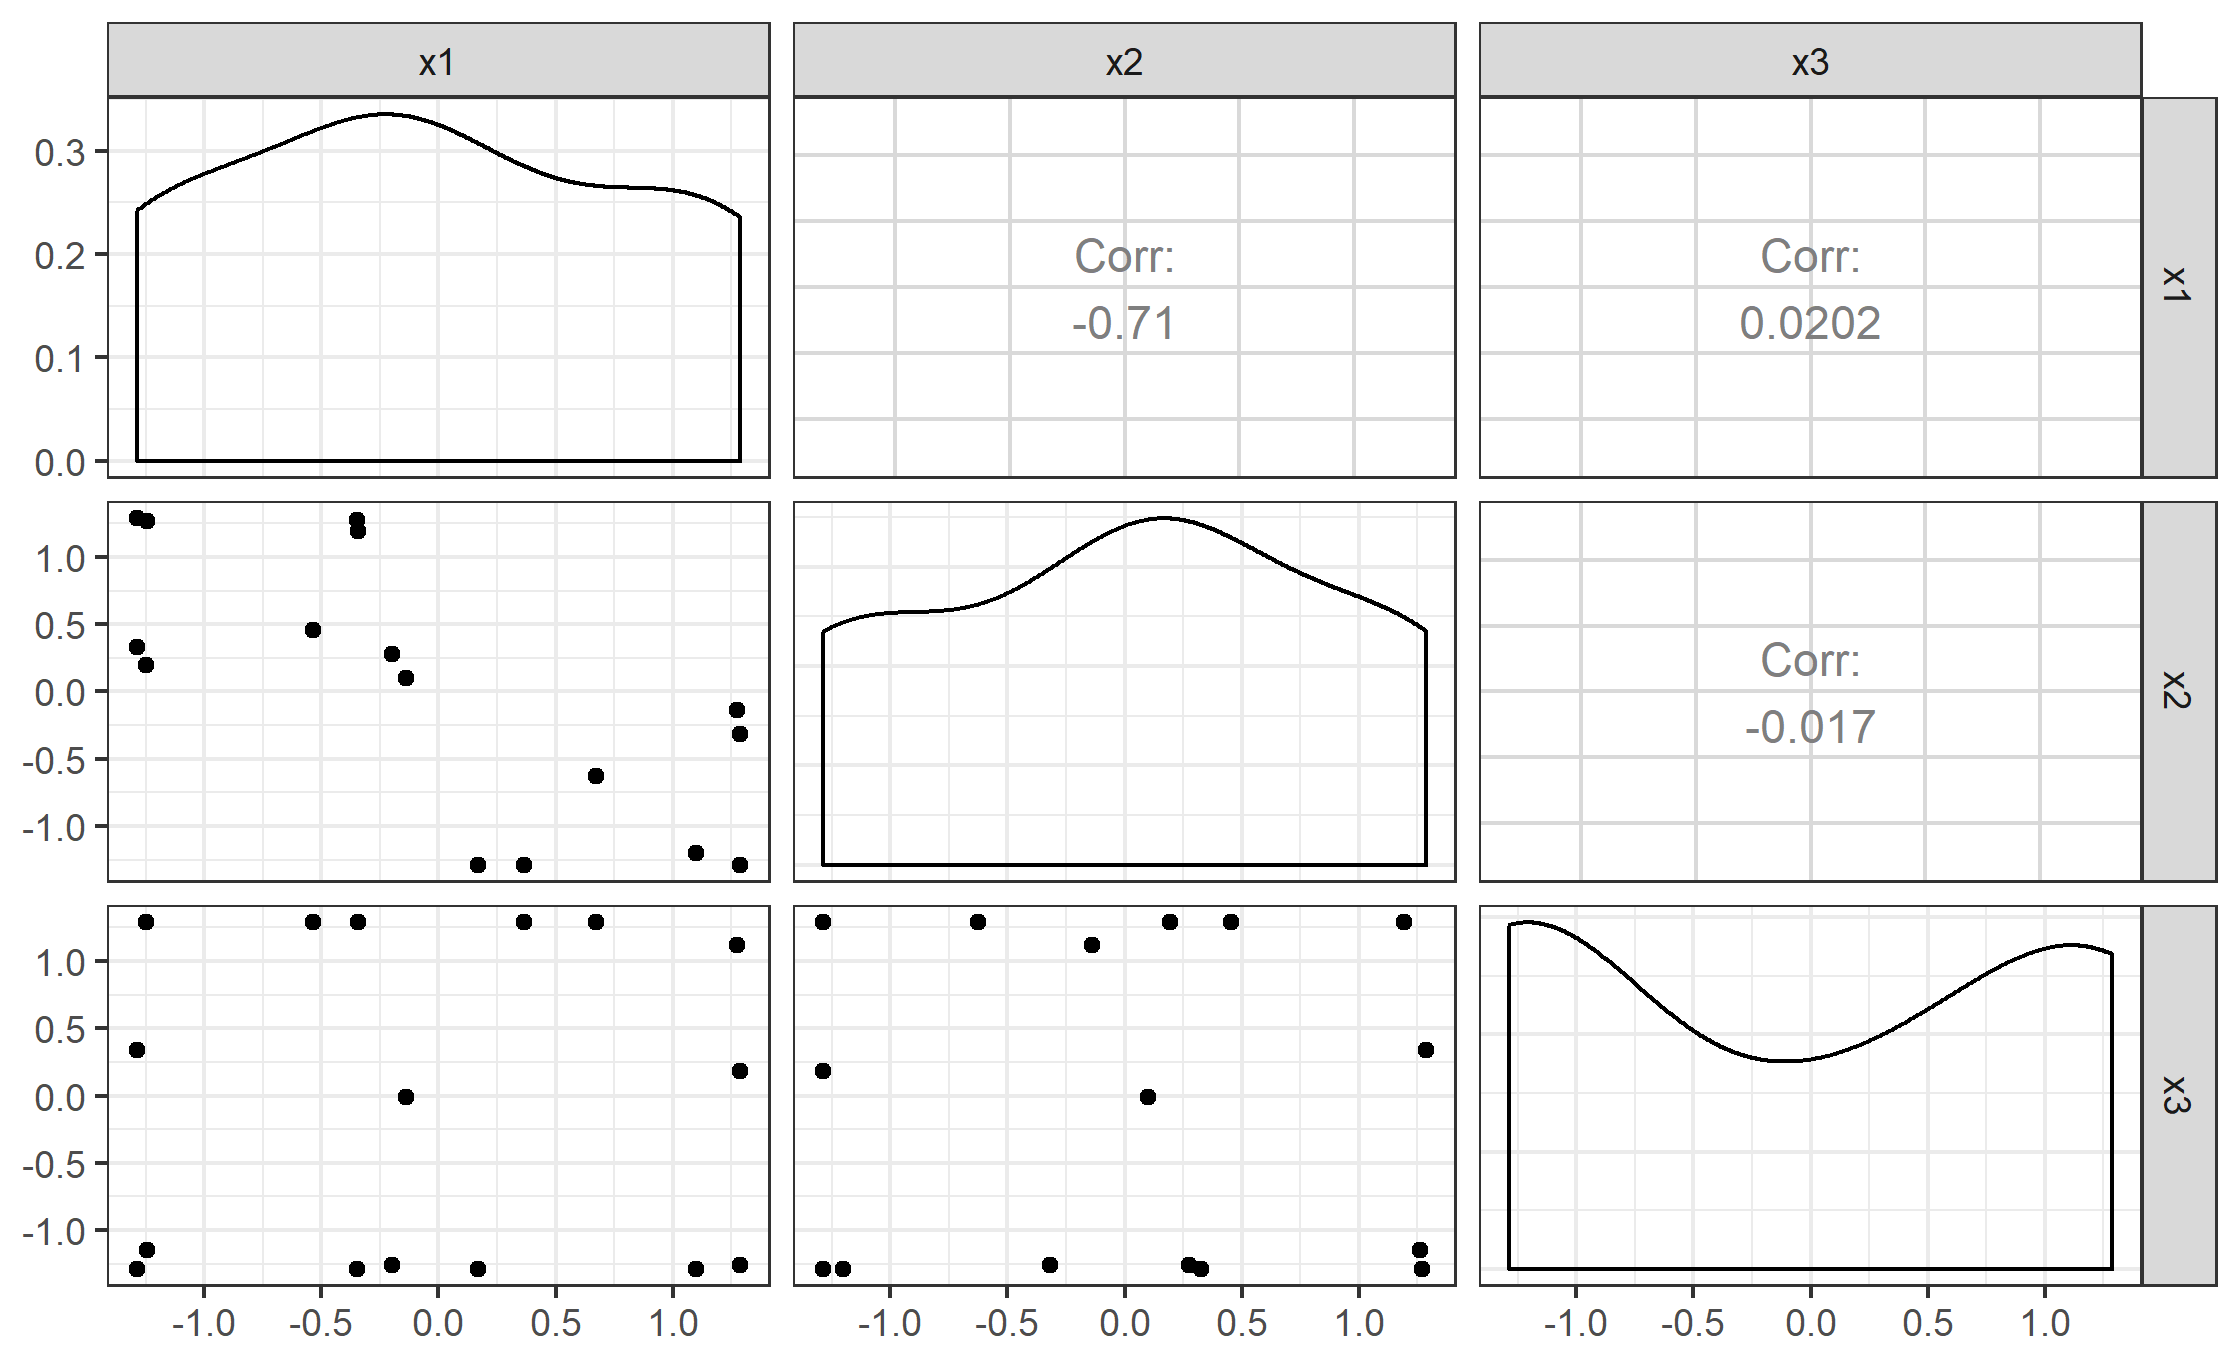
\includegraphics[width=\textwidth]{log_reg_fig_original}
    \caption{Se muestran proyecciones en una y dos dimensiones de las tres variables del modelo de regresión logística (\ref{eq:mod1_logistic_regression1}), así como su correlación.}
    \label{fig:log_reg_doe}
\end{figure}



Para corroborar la convergencia del algoritmo, la Figura \ref{fig:log_reg_conv} muestra una aproximación a la pérdida esperada del diseño en cuestión para cada una de las iteraciones de éste. Es inmediato observar que la pérdida esperada es prácticamente igual para las últimas iteraciones, lo que indica que, en efecto, el método convergió.


\begin{figure}[h]
	\centering
    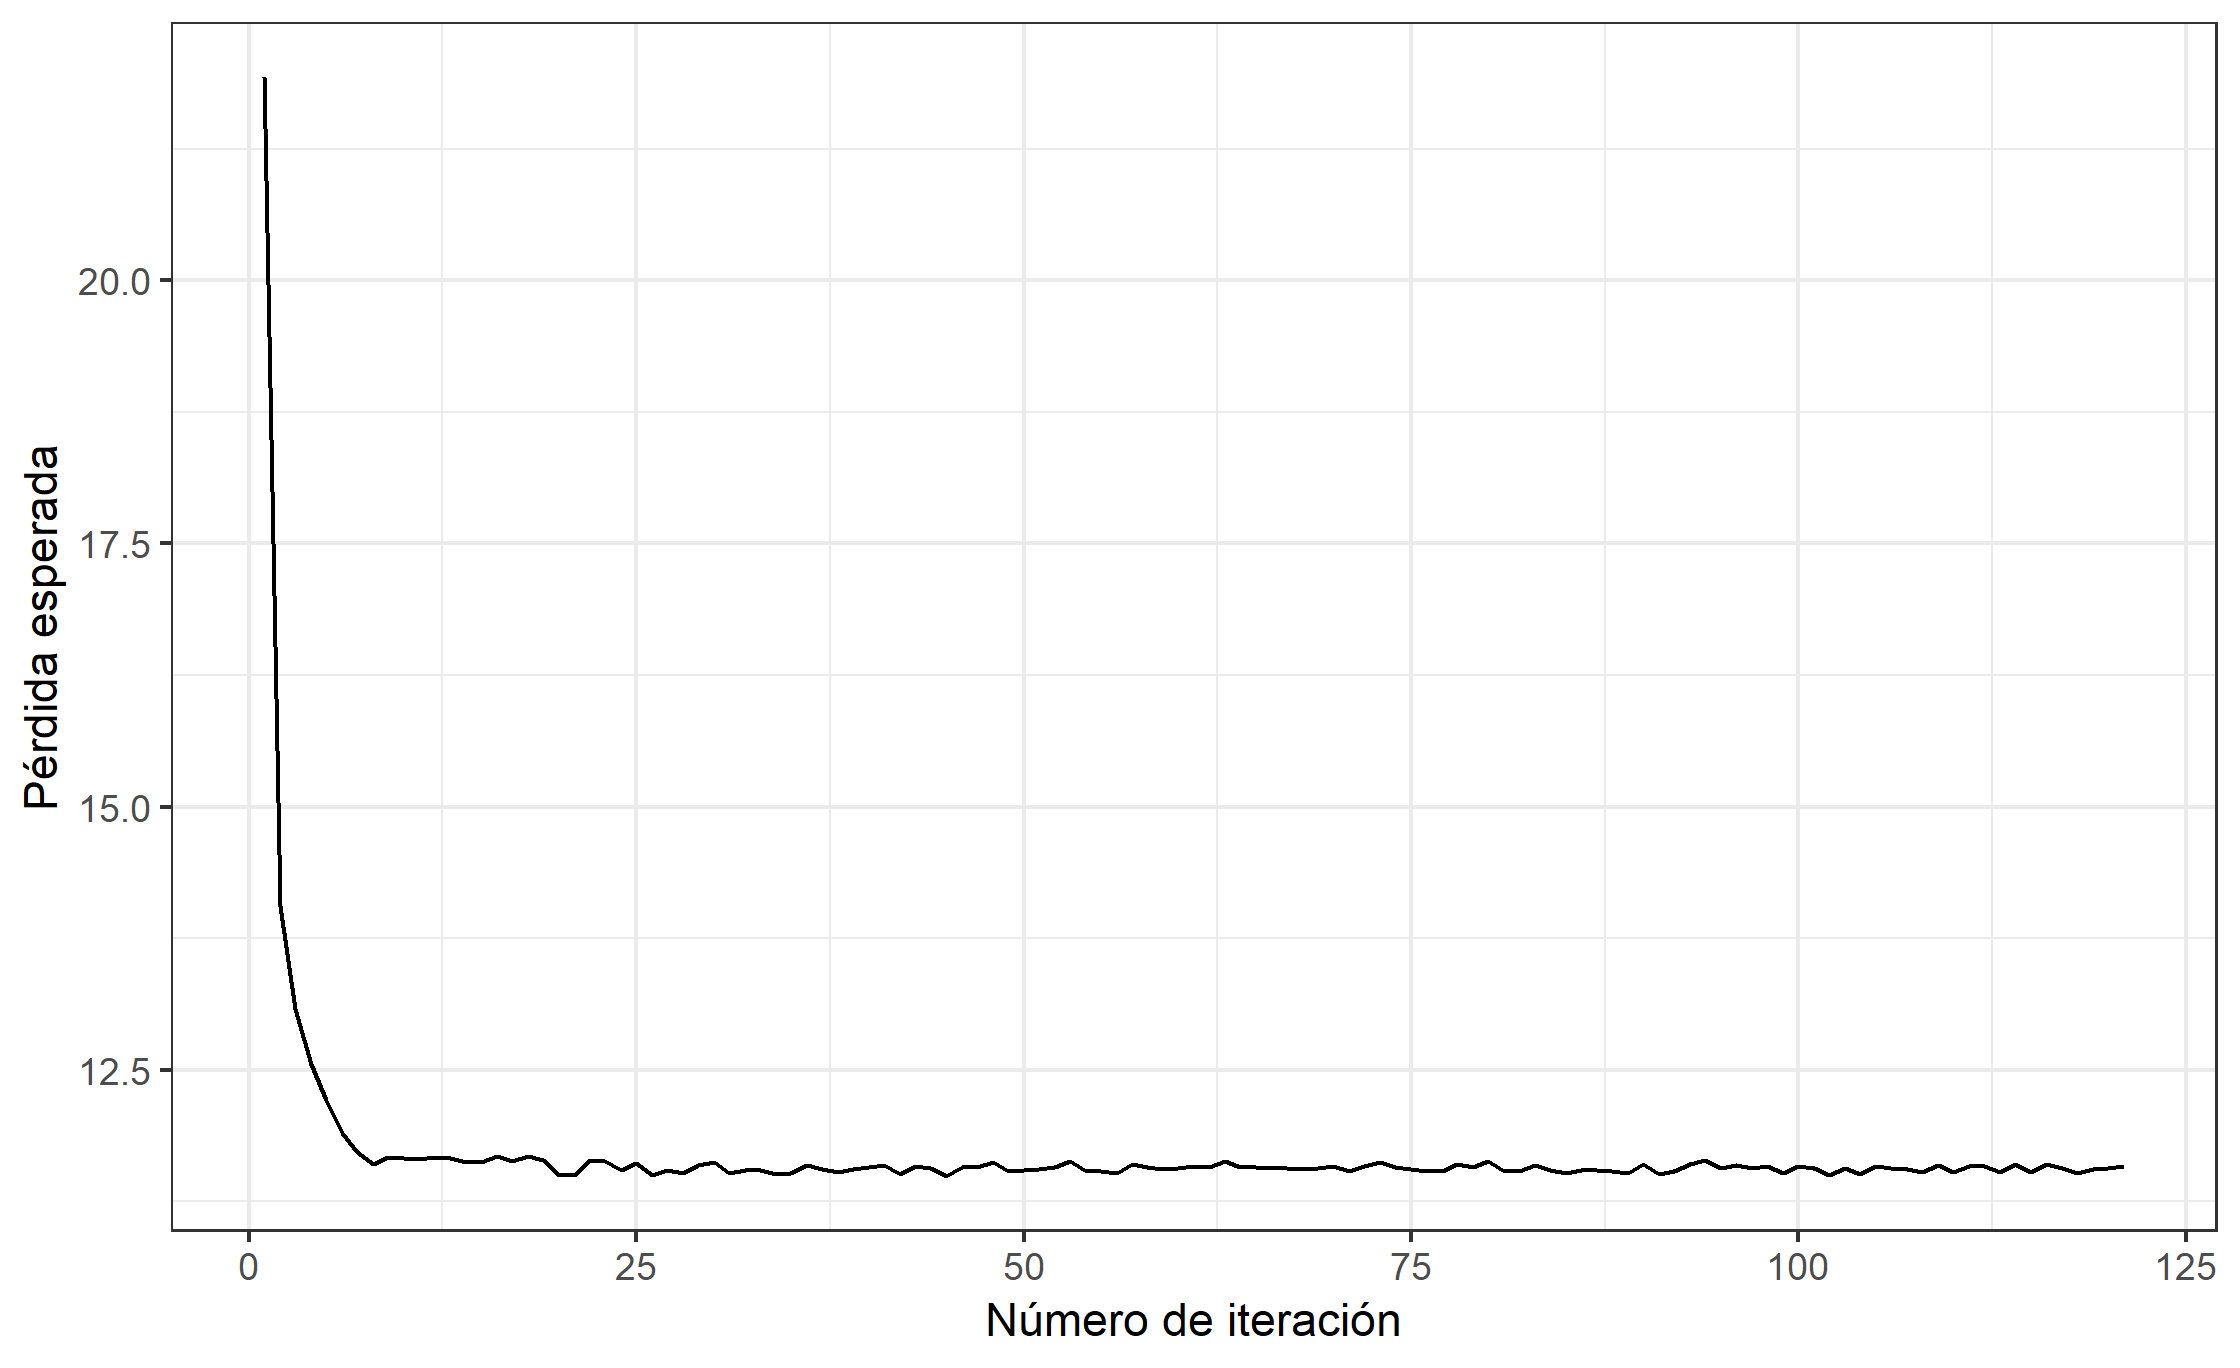
\includegraphics[width=\textwidth]{fig_conv_log_reg_original}
    \caption{Para la regresión logística (\ref{eq:mod1_logistic_regression1}), se muestran aproximaciones a la utilidad esperada de los diseños en cada iteración del algoritmo para corroborar convergencia.}
    \label{fig:log_reg_conv}
\end{figure}



\FloatBarrier


Para bosquejar la complejidad del problema es posible preguntarse qué forma toma la pérdida esperada. Dado que se encontró el diseño $D$~-óptimo Bayesiano, la pérdida esperada que este diseño minimiza está dada por
\begin{equation*}
	\Phi_{\text{D}} (\mathbf{x}) = \int_{\mathcal{Y}} \int_{B} \log \left( \frac{1}{p(\beta \, | \, y, \mathbf{x})} \right) p( \beta, y \, | \, \mathbf{x} ) \,d\beta \,dy,
\end{equation*}
donde $B = S_1 \times S_2 \times \cdots \times S_{10}$ es el espacio parametral y $S_i$ se refiere al soporte de $\beta_i$ (uno de (2, 6) o (-2,2)). Hay dos factores que entran en juego en este caso: la distribución posterior de $\beta$ y la distribución conjunta de $\beta$ e $y$. \\

La distribución posterior de $\beta$ depende tanto del diseño en cuestión $\mathbf{x}$ como de los datos $y$ que se observarán al realizar el experimento en las condiciones especificadas por $\mathbf{x}$. Por lo mismo no es inmediato obtener una expresión para $p(\beta \, | \, y, \mathbf{x})$, sino que se debe emplear el teorema de Bayes:
\begin{equation*}
	p(\beta \, | \, y, \mathbf{x}) = \frac{p(y \, | \, \beta, \mathbf{x}) \, p(\beta)}{p(y \, | \, \mathbf{x})}.
\end{equation*}
Esta expresión a su vez se divide en tres factores:
\begin{enumerate}
	\item $p(y \, | \, \beta, \mathbf{x})$ es la verosimilitud. Dado que los datos provienen independientemente de una distribución Bernoulli se tiene que
    \begin{align*}
    	p(y \, | \, \beta, \mathbf{x}) &= \prod_{i=1}^{16} \pi(\mathbf{x}_i)^{y_i} \, (1 - \pi(\mathbf{x}_i))^{1 - y_i} \\
        &= \prod_{i=1}^{16} \left( \frac{1}{1 + e^{-\eta_i}} \right)^{y_i} \, \left(1 - \frac{1}{1 + e^{-\eta_i}}  \right)^{1 - y_i}.
    \end{align*}
    No es posible simplificar esta expresión sin conocer los valores de los predictores, $\eta_i$.
    \item $p(\beta)$ es la distribución inicial conjunta de los parámetros. Por la independencia y distribuciones iniciales marginales de estos se tiene que
    \begin{align*}
    	p(\beta) &= \prod_{i=1}^{10} p(\beta_i) \\
        		 &= \left( \frac{1}{4} \right)^{10} \, \prod_{i=1}^{10} \mathds{1}_{S_i}(\beta_i),
    \end{align*}
    donde $\mathds{1}$ es la función indicadora.
    \item $p(y \, | \, \mathbf{x})$ es la función de densidad de los datos $y$, la cual se obtiene multiplicando las distribuciones de los puntos 1. y 2. e integrando sobre el espacio parametral $B$.
\end{enumerate}


La distribución conjunta de $\beta$ e $y$ también depende del diseño en cuestión y de los datos observados. Puntualmente
\begin{equation*}
	p( \beta, y \, | \, \mathbf{x} ) = p(\beta \, | \, y, \mathbf{x}) \, p(y \, | \, \mathbf{x}).
\end{equation*}
Esta expresión se divide a su vez en dos expresiones más, las cuales ya fueron discutidas previamente. Luego, para obtener la distribución conjunta es necesario \textit{(i)} obtener la distribución posterior de $\beta$ conjuntando los puntos 1. a 3., \textit{(ii)} obtener la densidad de $y$ dado $\mathbf{x}$ con el punto 3. y \textit{(iii)} multiplicar ambas distribuciones. \\


Habiendo obtenido estas componentes es aún necesario calcular el logaritmo del recíproco de la distribución posterior de $\beta$, multiplicarlo por la distribución conjunta de $\beta$ e $y$ y, posteriormente, evaluar la integral sobre todo el espacio parametral y luego sobre todo el espacio muestral. Si se quisiera encontrar el diseño óptimo entonces tendría que encontrarse analíticamente el mínimo de dicha expresión. \\

Evaluar la integral y minimizarla es claramente imposible, pero incluso tratar de obtener una expresión para el integrando es claramente una tarea compleja. Es por ello que, si se desean encontrar diseños no triviales, se \textit{debe} recurrir a herramientas computacionales como el método ACE. \\






Hay un punto que merece mayor discusión. La distribución inicial empleada por los autores para $\beta_1$ y $\beta_2$ es una distribución $\U (2, 6)$. Notoriamente el cero \textit{no} está contenido en el soporte de esta distribución. Lo que ello implica es que, al momento de obtener datos y conjuntar esta distribución inicial con la verosimilitud para así obtener la distribución final, el cero tampoco estará contenido en el soporte de la distribución final. En otras palabras, los autores están suponiendo que tanto $\beta_1$ como $\beta_2$ son diferentes de cero a priori. Y, más aún, este supuesto no cambiará independientemente de los datos observados. \\


Por otro lado, ni \cite{Woods_etal_2006} ni \cite{Woods_etal} dan alguna explicación clara sobre por qué supusieron que dichos coeficientes son distintos de cero. Por ello se volvió a encontrar el diseño $D$~-óptimo Bayesiano pero cambiando las distribuciones iniciales de estos dos parámetros, de forma que éstas fueran
\begin{align} \label{eq:mod1_params_initial_modified}
\begin{split}
	\beta_1, \beta_2 &\sim \U (-2, 6). 
\end{split}
\end{align}

No hay razón para modificar las demás distribuciones iniciales, ya que éstas sí contienen al cero en su soporte. Además, se dejó igual el límite superior del intervalo de $\beta_1$ y $\beta_2$, pero se modificó el límite inferior de forma que éste coincidiera con el de las demás distribuciones. Se utilizaron los mismos parámetros del método ACE que en el ejemplo anterior, es decir, $B=1,000$ y $Q = 10$ en el método ACE (Código \ref{code:ACE_Method}) y $\tilde{B} = 20,000$ en el algoritmo de aceptación y rechazo (Código \ref{code:ACE_AcceptReject}). La matriz de diseño óptima es
\begin{equation} \label{eq:logistic_regression_opt_design_modified}
	X_{\text{Modificada}}^{*} = \begin{bmatrix}
			    1.29 & -1.29 &  1.23 \\
			    1.29 & -1.27 & -1.27 \\
			    0.12 & -0.19 & -1.23 \\
			    0.44 & -1.29 &  0.06 \\
			    0.18 &  1.29 & -1.29 \\
			   -1.29 &  0.89 &  1.29 \\
			    1.27 &  0.55 & -1.27 \\
			   -1.15 &  1.29 & -1.11\\
			   -0.16 &  0.66 &  1.25\\
			   -0.33 &  0.13 & -0.05 \\
			    1.28 &  1.29 &  1.29 \\
			   -0.44 & -1.29 & -1.29 \\
			   -1.29 & -0.03 & -1.29 \\
			   -1.29 & -0.86 &  1.21 \\
			    0.09 & -0.46 &  1.29 \\
			    1.13 & -0.09 &  0.42
	      \end{bmatrix}
\end{equation}

Es de observar que el hecho de modificar las distribuciones iniciales derivó en un diseño óptimo diferente. Para obtener conclusiones de mayor profundidad la Figura \ref{fig:log_reg_doe_modified} es análoga a la Figura \ref{fig:log_reg_doe}, y muestra las proyecciones de las variables en una y dos dimensiones (con un suavizamiento para mostrar densidad en la primera de ellas) y las correlaciones. \\







\begin{figure}[h]
	\centering
    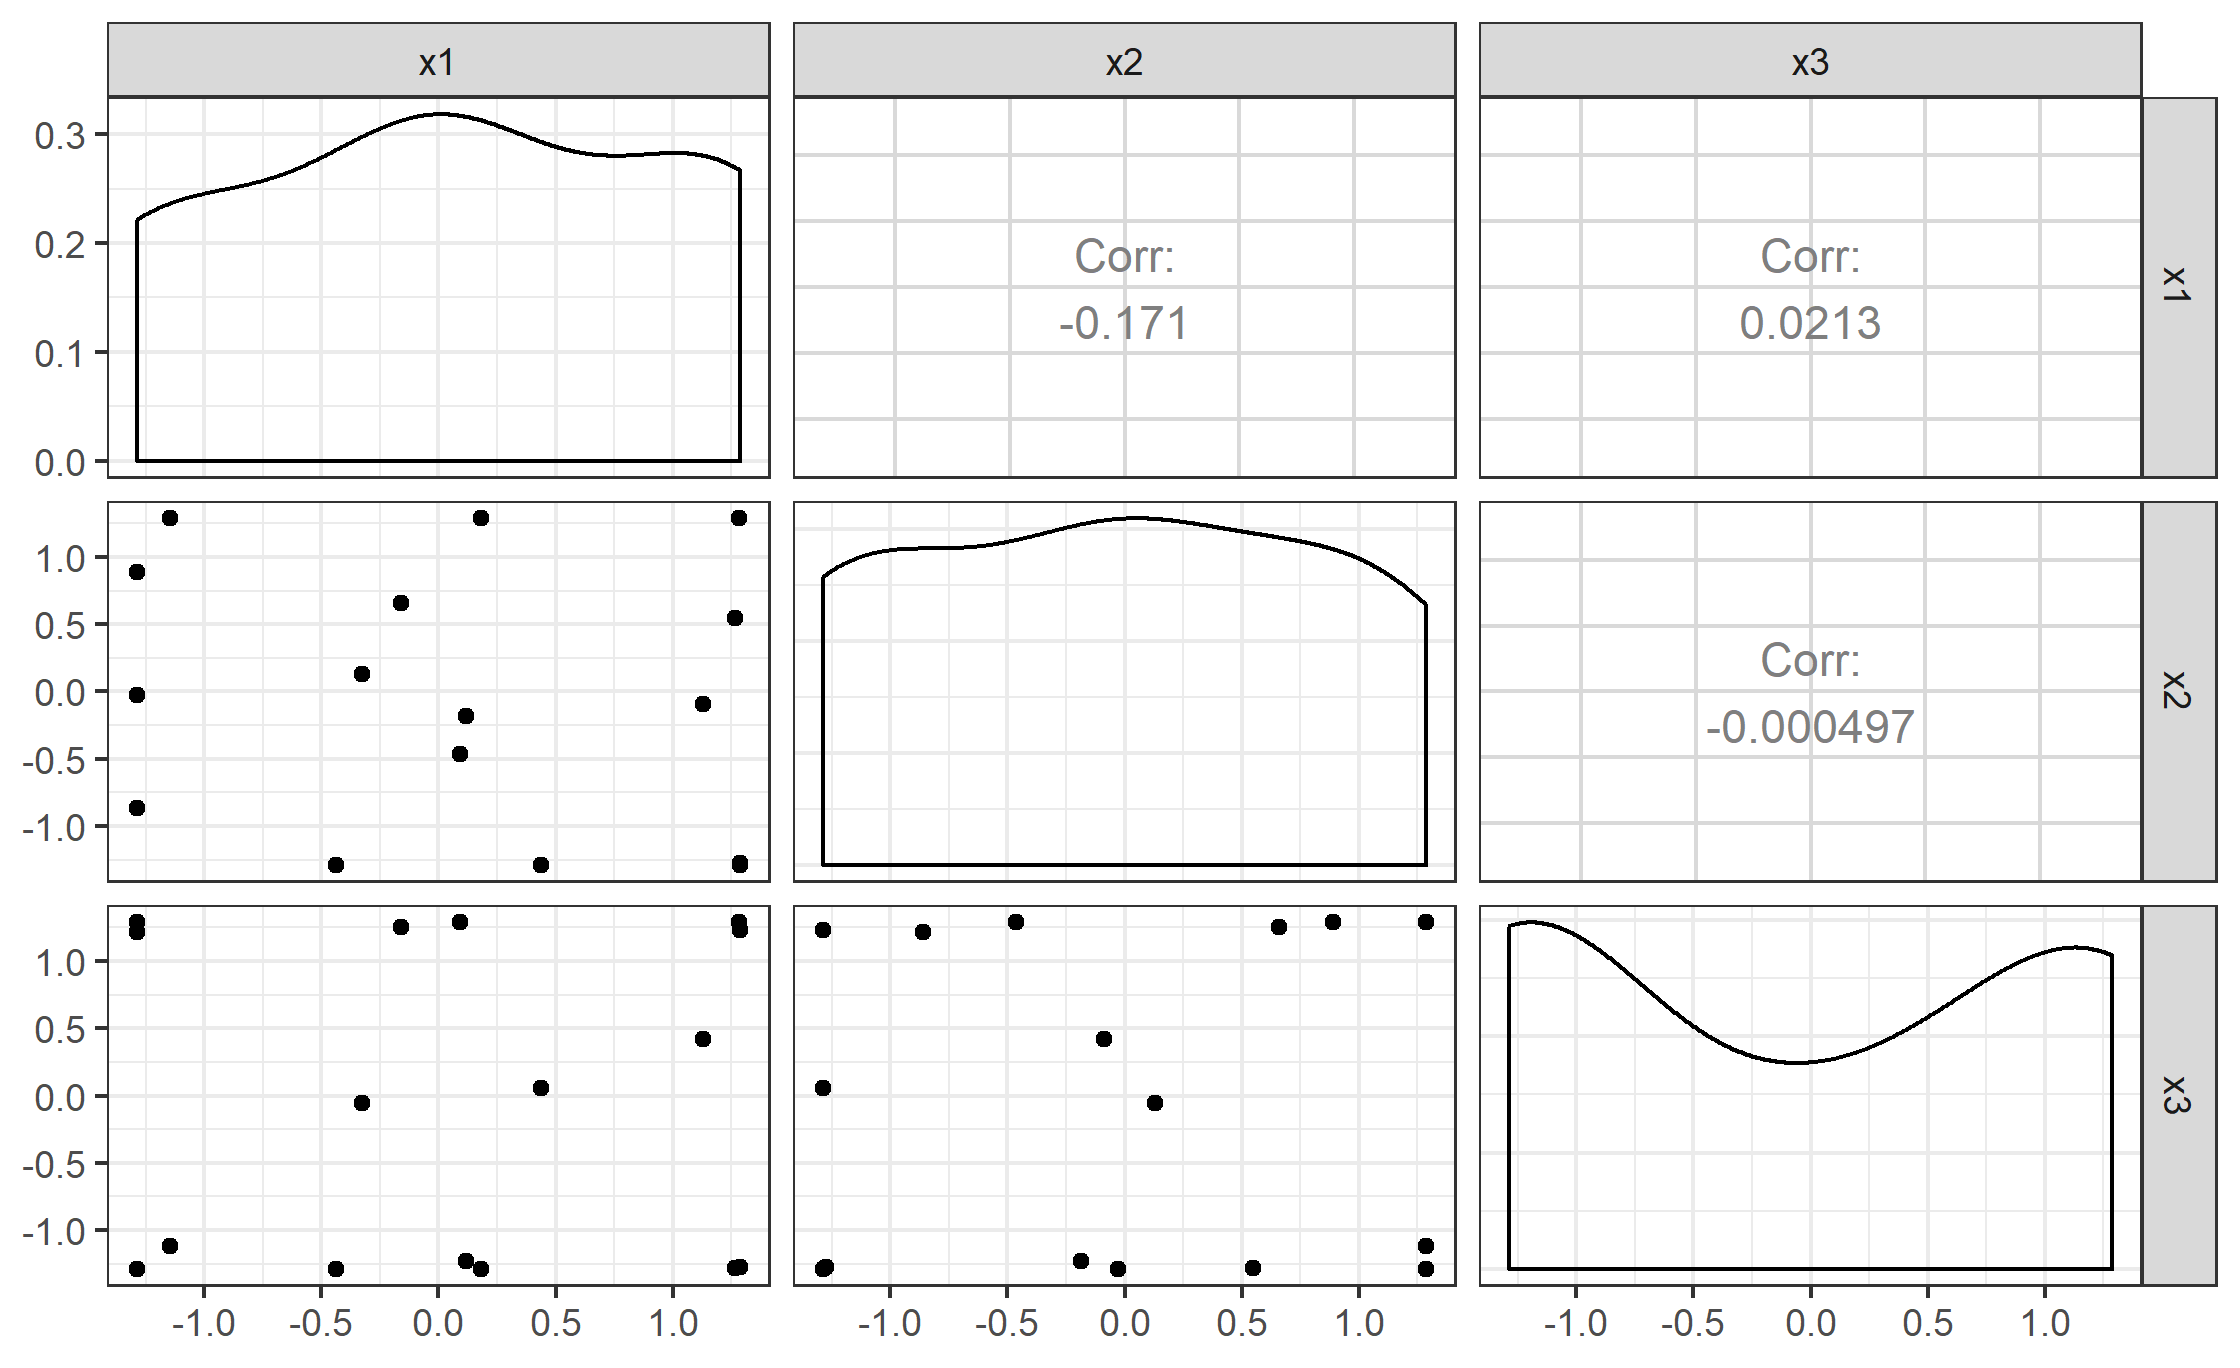
\includegraphics[width=\textwidth]{log_reg_fig_modified}
    \caption{Se muestran proyecciones en una y dos dimensiones de las tres variables del modelo de regresión logística (\ref{eq:mod1_logistic_regression1}) con distribuciones iniciales modificadas (\ref{eq:mod1_params_initial_modified}), así como su correlación.}
    \label{fig:log_reg_doe_modified}
\end{figure}








Hay algunas diferencias con respecto al diseño óptimo original que comentar. Primeramente la covariable $x_3$ sufrió pocos cambios, en tanto que su densidad suavizada se mantuvo prácticamente igual y sigue concentrada en los extremos del espacio muestral. En el caso de $x_2$, sin embargo, la densidad pasó de estar concentrada alrededor del cero a estar distribuida uniformemente en el espacio muestral. \\


Por otro lado es interesante observar que las correlaciones entre $x_3$ y el resto de las covariables se mantuvieron relativamente similares, siendo ambas cercanas a cero. Sin embargo, la correlación entre $x_1$ y $x_2$ cambió drásticamente, puesto que dichas variables pasaron de estar altamente correlacionadas (-0.71) a estar solo un poco correlacionadas (-0.17). Resumiendo, modificar las distribuciones iniciales de $\beta_1$ y $\beta_2$ tuvo un impacto directo en $x_1$ y $x_2$, mas no en $x_3$, lo cual tiene sentido. \\



De nuevo para corroborar la convergencia del algoritmo, la Figura \ref{fig:log_reg_conv_modified} muestra una aproximación a la pérdida esperada del diseño en cuestión para cada una de las iteraciones de éste. Es inmediato observar que la pérdida esperada es prácticamente igual para las últimas iteraciones, señal de 
convergencia en el método.


\begin{figure}[h]
	\centering
    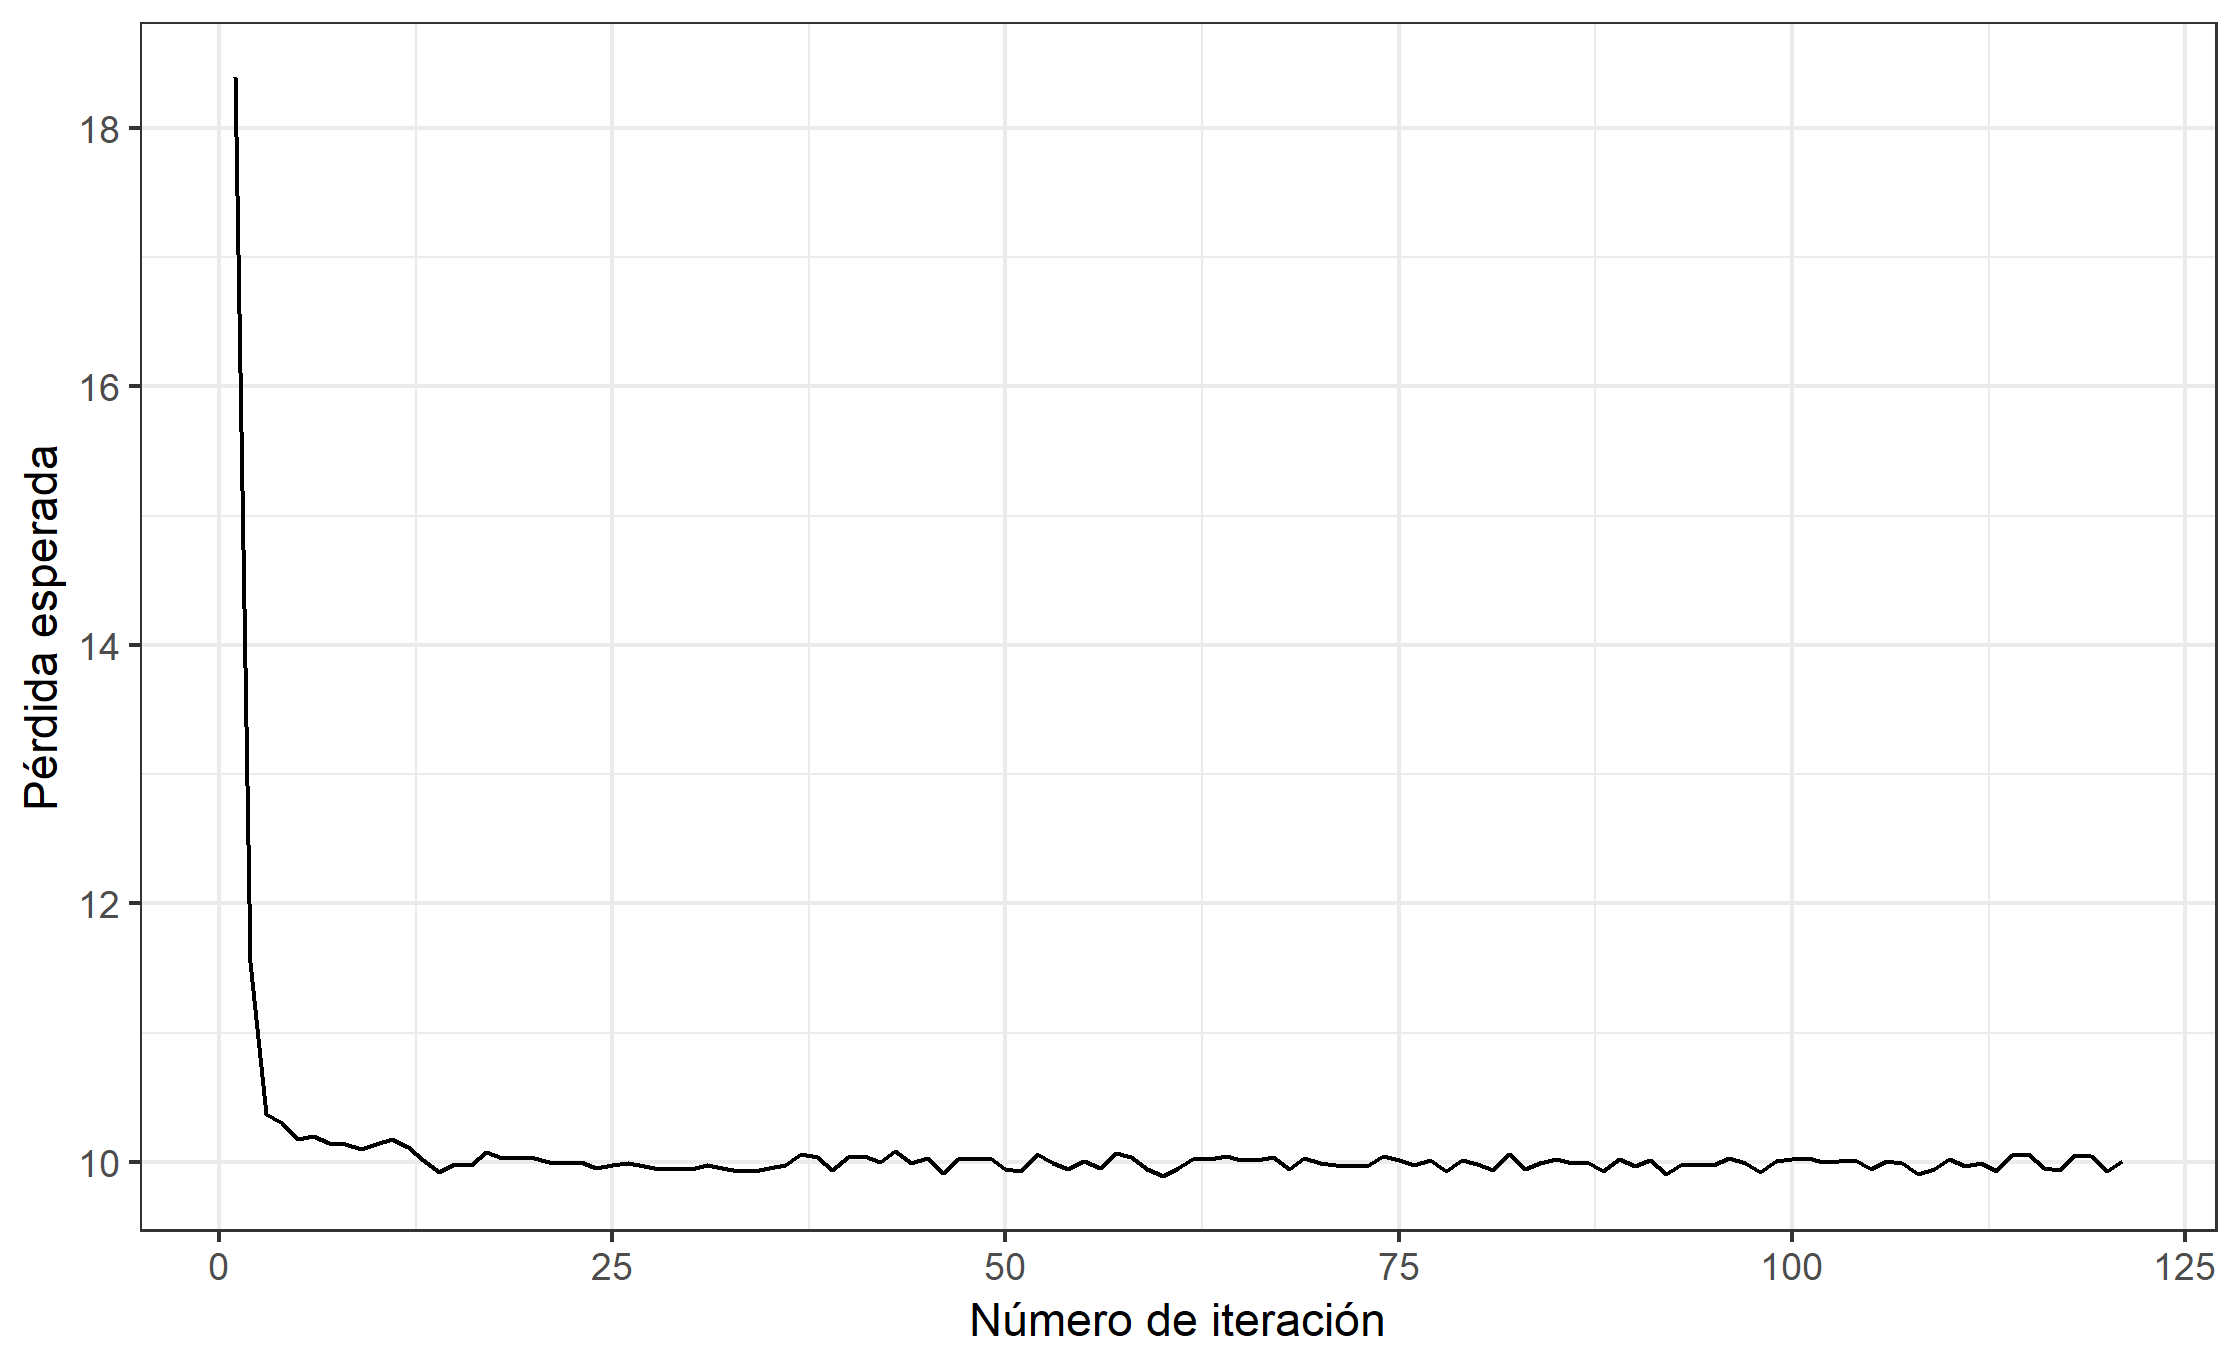
\includegraphics[width=\textwidth]{fig_conv_log_reg_modified}
    \caption{Para la regresión logística (\ref{eq:mod1_logistic_regression1}) con distribuciones iniciales modificadas (\ref{eq:mod1_params_initial_modified}), se muestran aproximaciones a la utilidad esperada de los diseños en cada iteración del algoritmo para corroborar convergencia.}
    \label{fig:log_reg_conv_modified}
\end{figure}


\FloatBarrier








\section{Diseño para modelo de regresión Poisson}



A lo largo de la historia siempre ha sido de interés modelar el número de ocurrencias de un fenómeno en cierto periodo de tiempo. La distribución Poisson es una de las alternativas más populares para este tipo de situaciones, y la familia de modelos lineales generalizados que suponen dicha distribución en la respuesta ha sido altamente estudiada. De particular interés es el modelo que utiliza la liga canónica (logarítmica), la cual se discutió con detalle en el Capítulo \ref{chapter:glms}. \\

%\newpage

\cite{atkinson_woods} encuentran resultados teóricos importantes para el diseño experimental para modelos de regresión Poisson. \cite{Woods_etal} retoman y aprovechan dichos resultados, asumiendo que se tiene un experimento con $n=6$ ensayos para cinco variables $x_1, ..., x_5$. Sea $Y_i \sim \Pois(\lambda(x_i))$. Entonces se pretende modelar
\begin{equation} \label{eq:mod2_poisson_regression1}
	\log \lambda(x_i) = \beta_0 + \sum_{j=1}^{5} \beta_j x_{ij}, \quad i=1,...,6,
\end{equation}
aprovechando que $\lambda(x_i) = \mu(x_i)$ en el modelo Poisson.\\


Más aún, los autores asumen que $\beta_0 = 0$ es conocido. 	Las distribuciones iniciales para los demás parámetros son independientes y están dadas por
\begin{align} \label{eq:mod2_params_initial}
\begin{split}
	\beta_1, \beta_3, \beta_5 &\sim \mathcal{U}(1, 1+\alpha),\\
    \beta_2, \beta_4 &\sim \mathcal{U}(-1-\alpha, -1),
\end{split}
\end{align}
donde $\alpha > 0$ es un parámetro fijo. Las covariables toman valores en $[-1, 1]^5$, utilizando la notación del ejemplo anterior. Los demás argumentos del método ACE utilizados por los autores son $B=1,000$ y $Q = 20$ en el método ACE (Código \ref{code:ACE_Method}) y $\tilde{B} = 20,000$ en el algoritmo de aceptación y rechazo (Código \ref{code:ACE_AcceptReject}). \\

Woods et al. encuentran el diseño SIL-óptimo para los valores ${\alpha = 0.5}$ y ${\alpha = 0.75}$. Para comparar con sus resultados se encontró el diseño $D$~-óptimo.
La Tabla \ref{table:alfa5} muestra la comparación del diseño SIL-óptimo con el $D$~-óptimo para $\alpha = 0.5$, y la Tabla \ref{table:alfa75} muestra lo respectivo para $\alpha = 0.75$.


\begin{table}[h]
\small
\centering
\begin{tabular}{l|lllll|lllll}
\multirow{2}{*}{Núm} & \multicolumn{5}{l|}{ \hspace{1.2cm} Diseño $D$~-óptimo} & \multicolumn{5}{l}{  \hspace{1cm}  Diseño SIL-óptimo}  \\
                     & $x_1$  & $x_2$ & $x_3$ & $x_4$ & $x_5$ & $x_1$ & $x_2$ & $x_3$ & $x_4$ & $x_5$  \\ \hline
1                    & -0.42  & -1    & 1     & -1    & 1     & -0.5  & -1    & 1     & -1    & 1      \\
2                    & 1      & 0.5  & 1     & -1    & 1     & 1     & 0.56  & 1     & -1    & 1      \\
3                    & 1      & -1    & -0.36  & -1    & 1     & 1     & -1    & -0.31 & -1    & 1      \\
4                    & 1      & -1    & 1     & 0.51  & 1     & 1     & -1    & 1     & 0.33  & 1      \\
5                    & 1      & -1    & 1     & -1    & -0.39 & 1     & -1    & 1     & -1    & -0.38 \\
6                    & 1      & -1    & 1     & -1    & 1     & 1     & -1    & 1     & -1    & 1     
\end{tabular}
\caption{Se muestran los diseños óptimos según los dos distintos criterios para $\alpha = 0.5$.}
\label{table:alfa5}
\end{table}



\begin{table}[h]
\small
\centering
\begin{tabular}{l|lllll|lllll}
\multirow{2}{*}{Núm} & \multicolumn{5}{l|}{ \hspace{1.2cm} Diseño $D$~-óptimo} & \multicolumn{5}{l}{  \hspace{1cm}  Diseño SIL-óptimo}  \\
                     & $x_1$  & $x_2$ & $x_3$ & $x_4$ & $x_5$ & $x_1$ & $x_2$ & $x_3$ & $x_4$ & $x_5$  \\ \hline
1                    & -0.32  & -1    & 1     & -1    & 1     & -0.22  & -1    & 1     & -1    & 1      \\
2                    & 1      & 0.34  & 1     & -1    & 1     & 1     & 0.22  & 1     & -1    & 1      \\
3                    & 1      & -1    & -0.34  & -1    & 1     & 1     & -1    & -0.32 & -1    & 1      \\
4                    & 1      & -1    & 1     & 0.38  & 1     & 1     & -1    & 1     & 0.11  & 1      \\
5                    & 1      & -1    & 1     & -1    & -0.47 & 1     & -1    & 1     & -1    & -0.31 \\
6                    & 1      & -1    & 1     & -1    & 1     & 1     & -1    & 1     & -1    & 1     
\end{tabular}
\caption{Se muestran los diseños óptimos según los dos distintos criterios para $\alpha = 0.75$.}
\label{table:alfa75}
\end{table}


En ambos casos las variables toman el mismo valor, ya sea $\pm 1$, en todos los ensayos menos uno: el que aparece en la diagonal.\footnote{Aunque en estricto sentido no se puede hablar de una diagonal, se entiende que se refiere al valor $x_{ii}$ de la covariable.} Es ahí donde se aprecian las diferencias entre ambos diseños óptimos. Si bien es cierto que los signos son todos iguales, también se vislumbran pequeñas diferencias entre los valores de las variables del diseño óptimo. En particular, $x_4$ es la covariable que muestra mayor variación para ambos valores de $\alpha$. Esto se debe a que distintos criterios de optimalidad llevan a distintos diseños óptimos. Sin embargo cabe recordar que la $D$~-optimalidad Bayesiana es similar a la SIL~-optimalidad, lo que explica que ambos diseños sean relativamente similares. \\



Las Figuras \ref{fig:pois_reg5} y \ref{fig:pois_reg75} muestran las proyecciones en dos dimensiones de las variables junto con su proyección en una dimensión (en forma de densidad), para $\alpha=0.5$ y $\alpha=0.75$. Además se muestran las correlaciones que tendrán las covariables empleando el diseño óptimo. Es interesante que éstas son todas iguales a $\pm 0.2$ para ambos valores de $\alpha$. Ello indica que el diseño óptimo de nuevo no considera utilizar covariables no correlacionadas y, más aún, que la correlación entre las variables siempre será de $\pm 0.2$. \\







\begin{figure}[h]
	\centering
    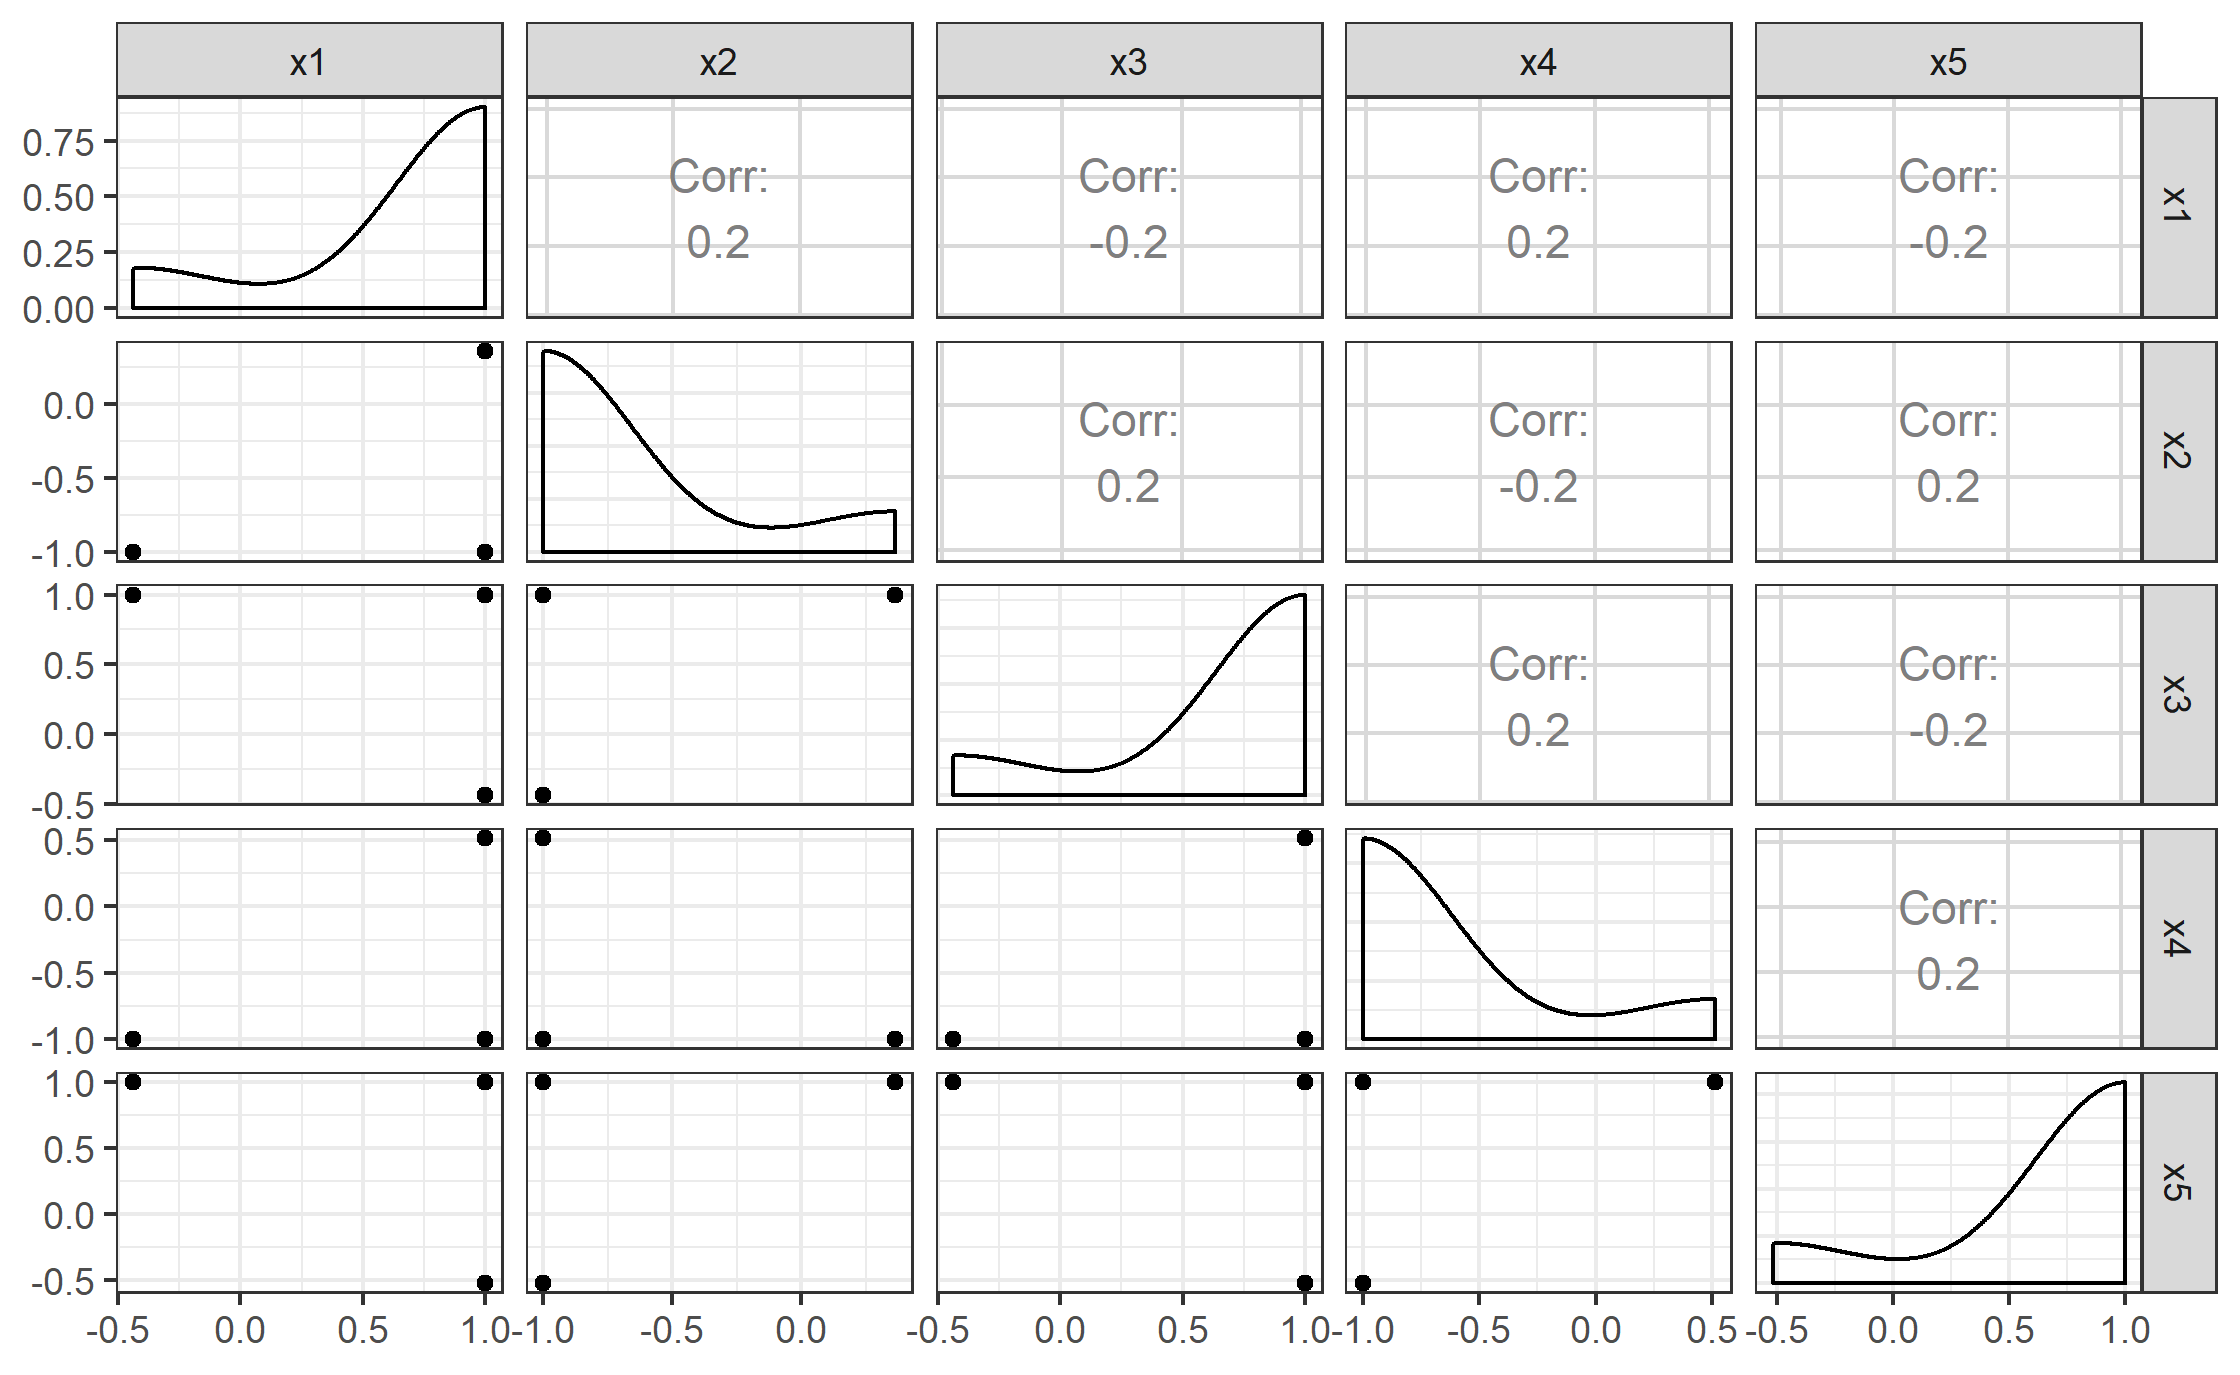
\includegraphics[width=\textwidth]{alpha_50_original.png}
    \caption{Se muestran proyecciones en una y dos dimensiones de las tres variables del modelo de regresión Poisson (\ref{eq:mod2_poisson_regression1}), así como su correlación, para $\alpha=0.5$.}
    \label{fig:pois_reg5}
\end{figure}



\begin{figure}[h]
	\centering
    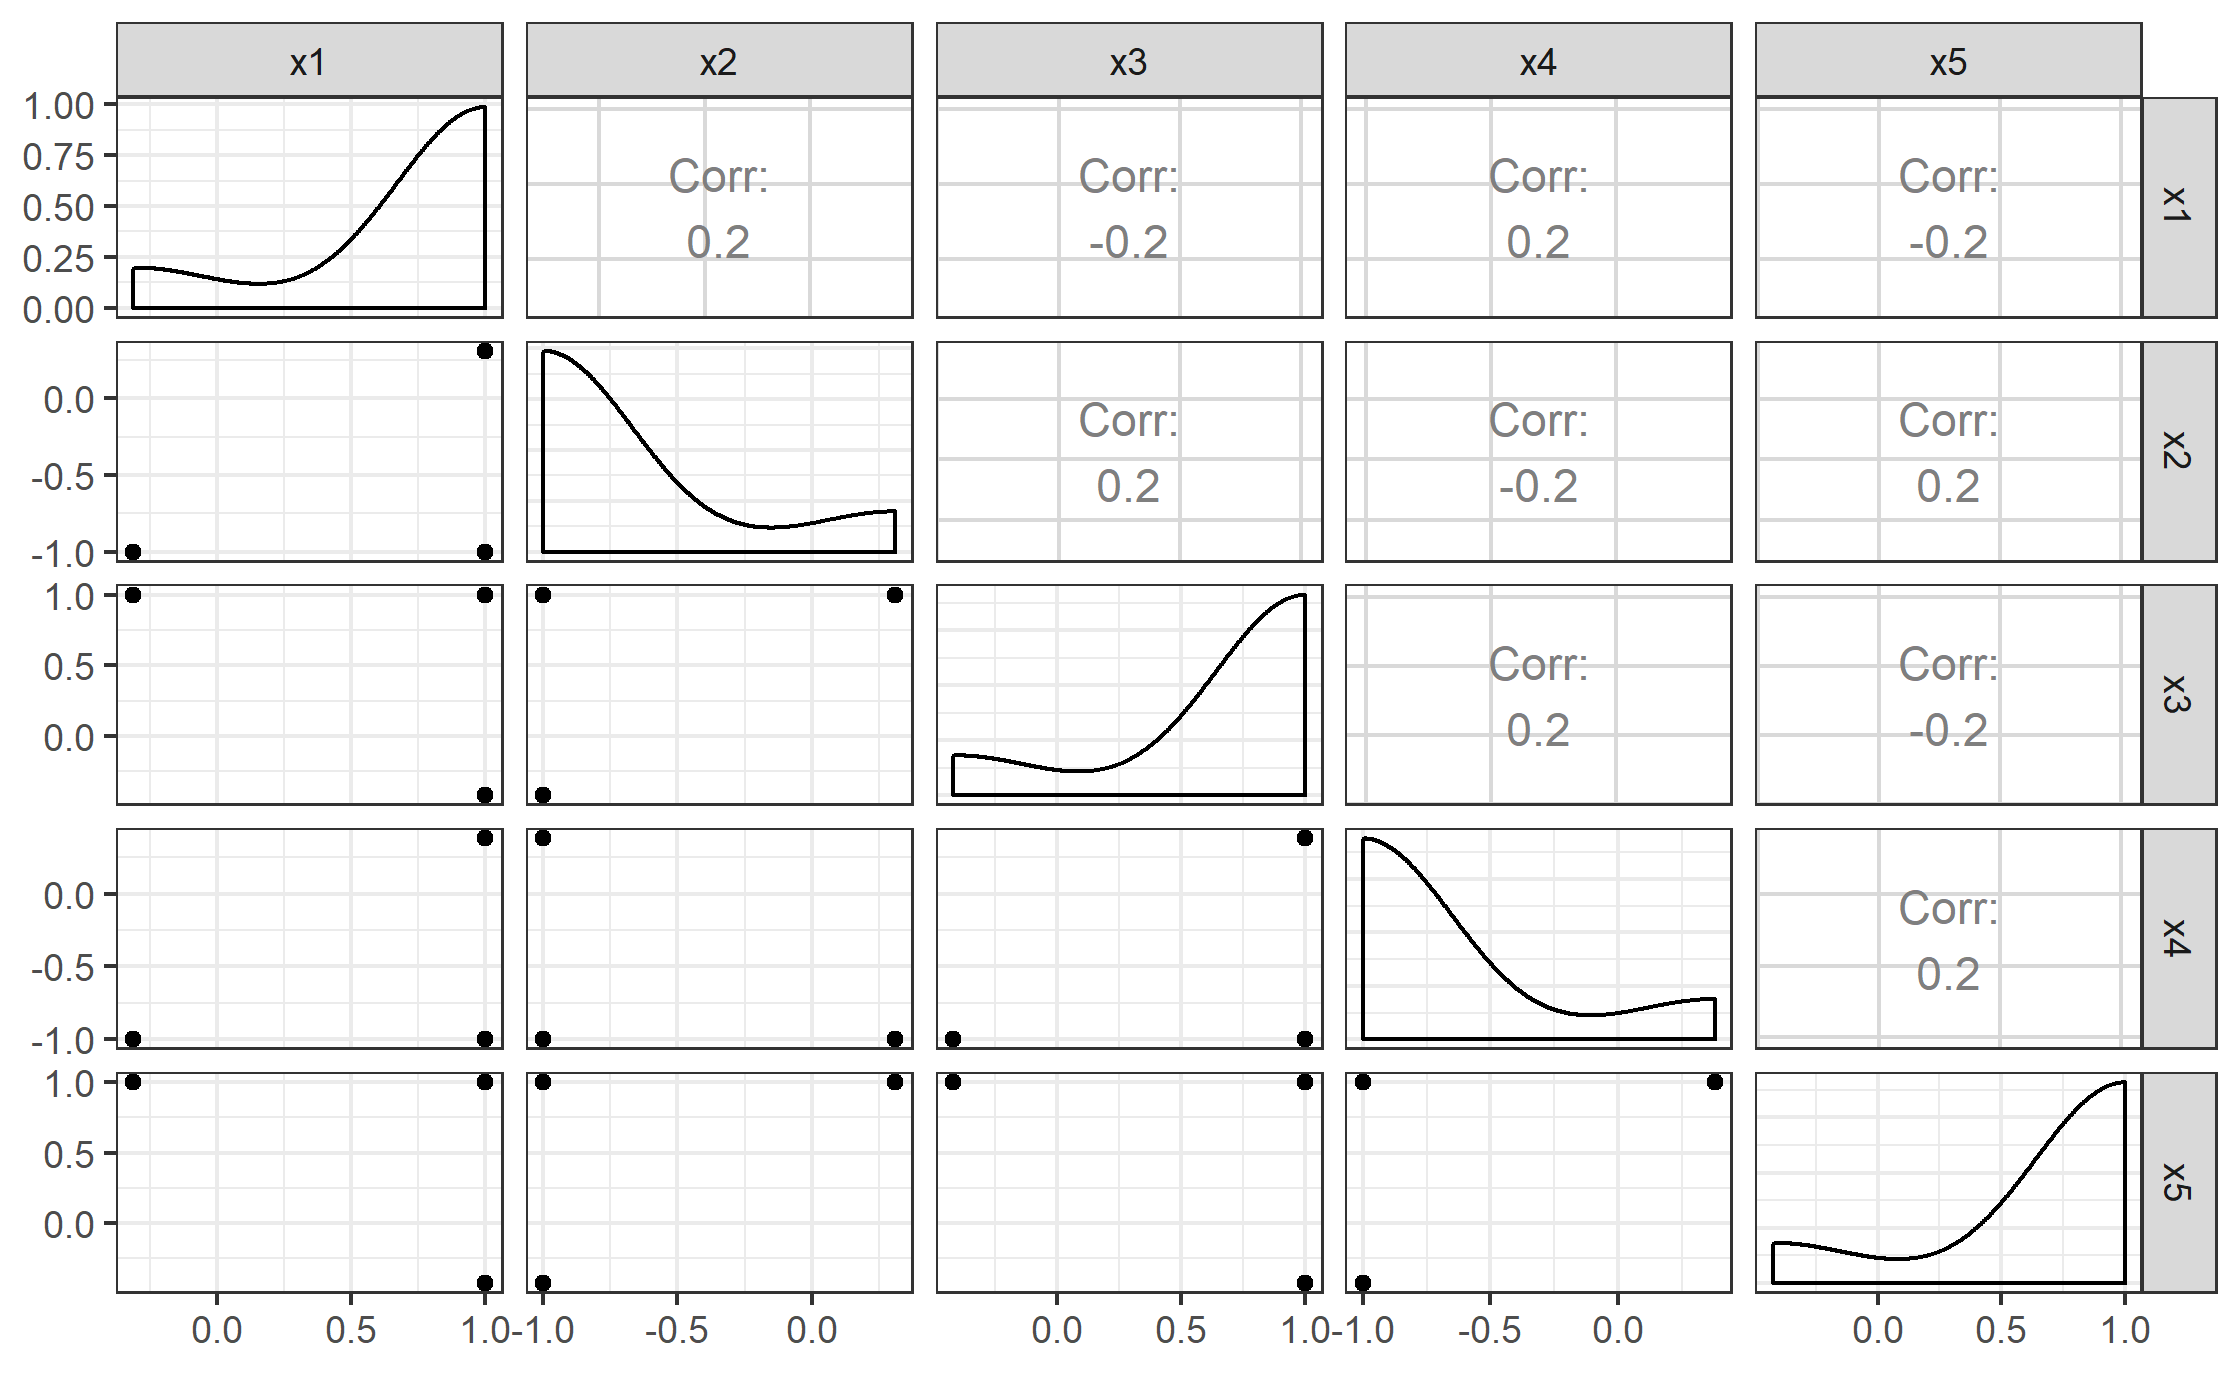
\includegraphics[width=\textwidth]{alpha_75_original.png}
    \caption{Se muestran proyecciones en una y dos dimensiones de las tres variables del modelo de regresión Poisson (\ref{eq:mod2_poisson_regression1}), así como su correlación, para $\alpha=0.75$.}
    \label{fig:pois_reg75}
\end{figure}




\begin{figure}[h]
	\centering
    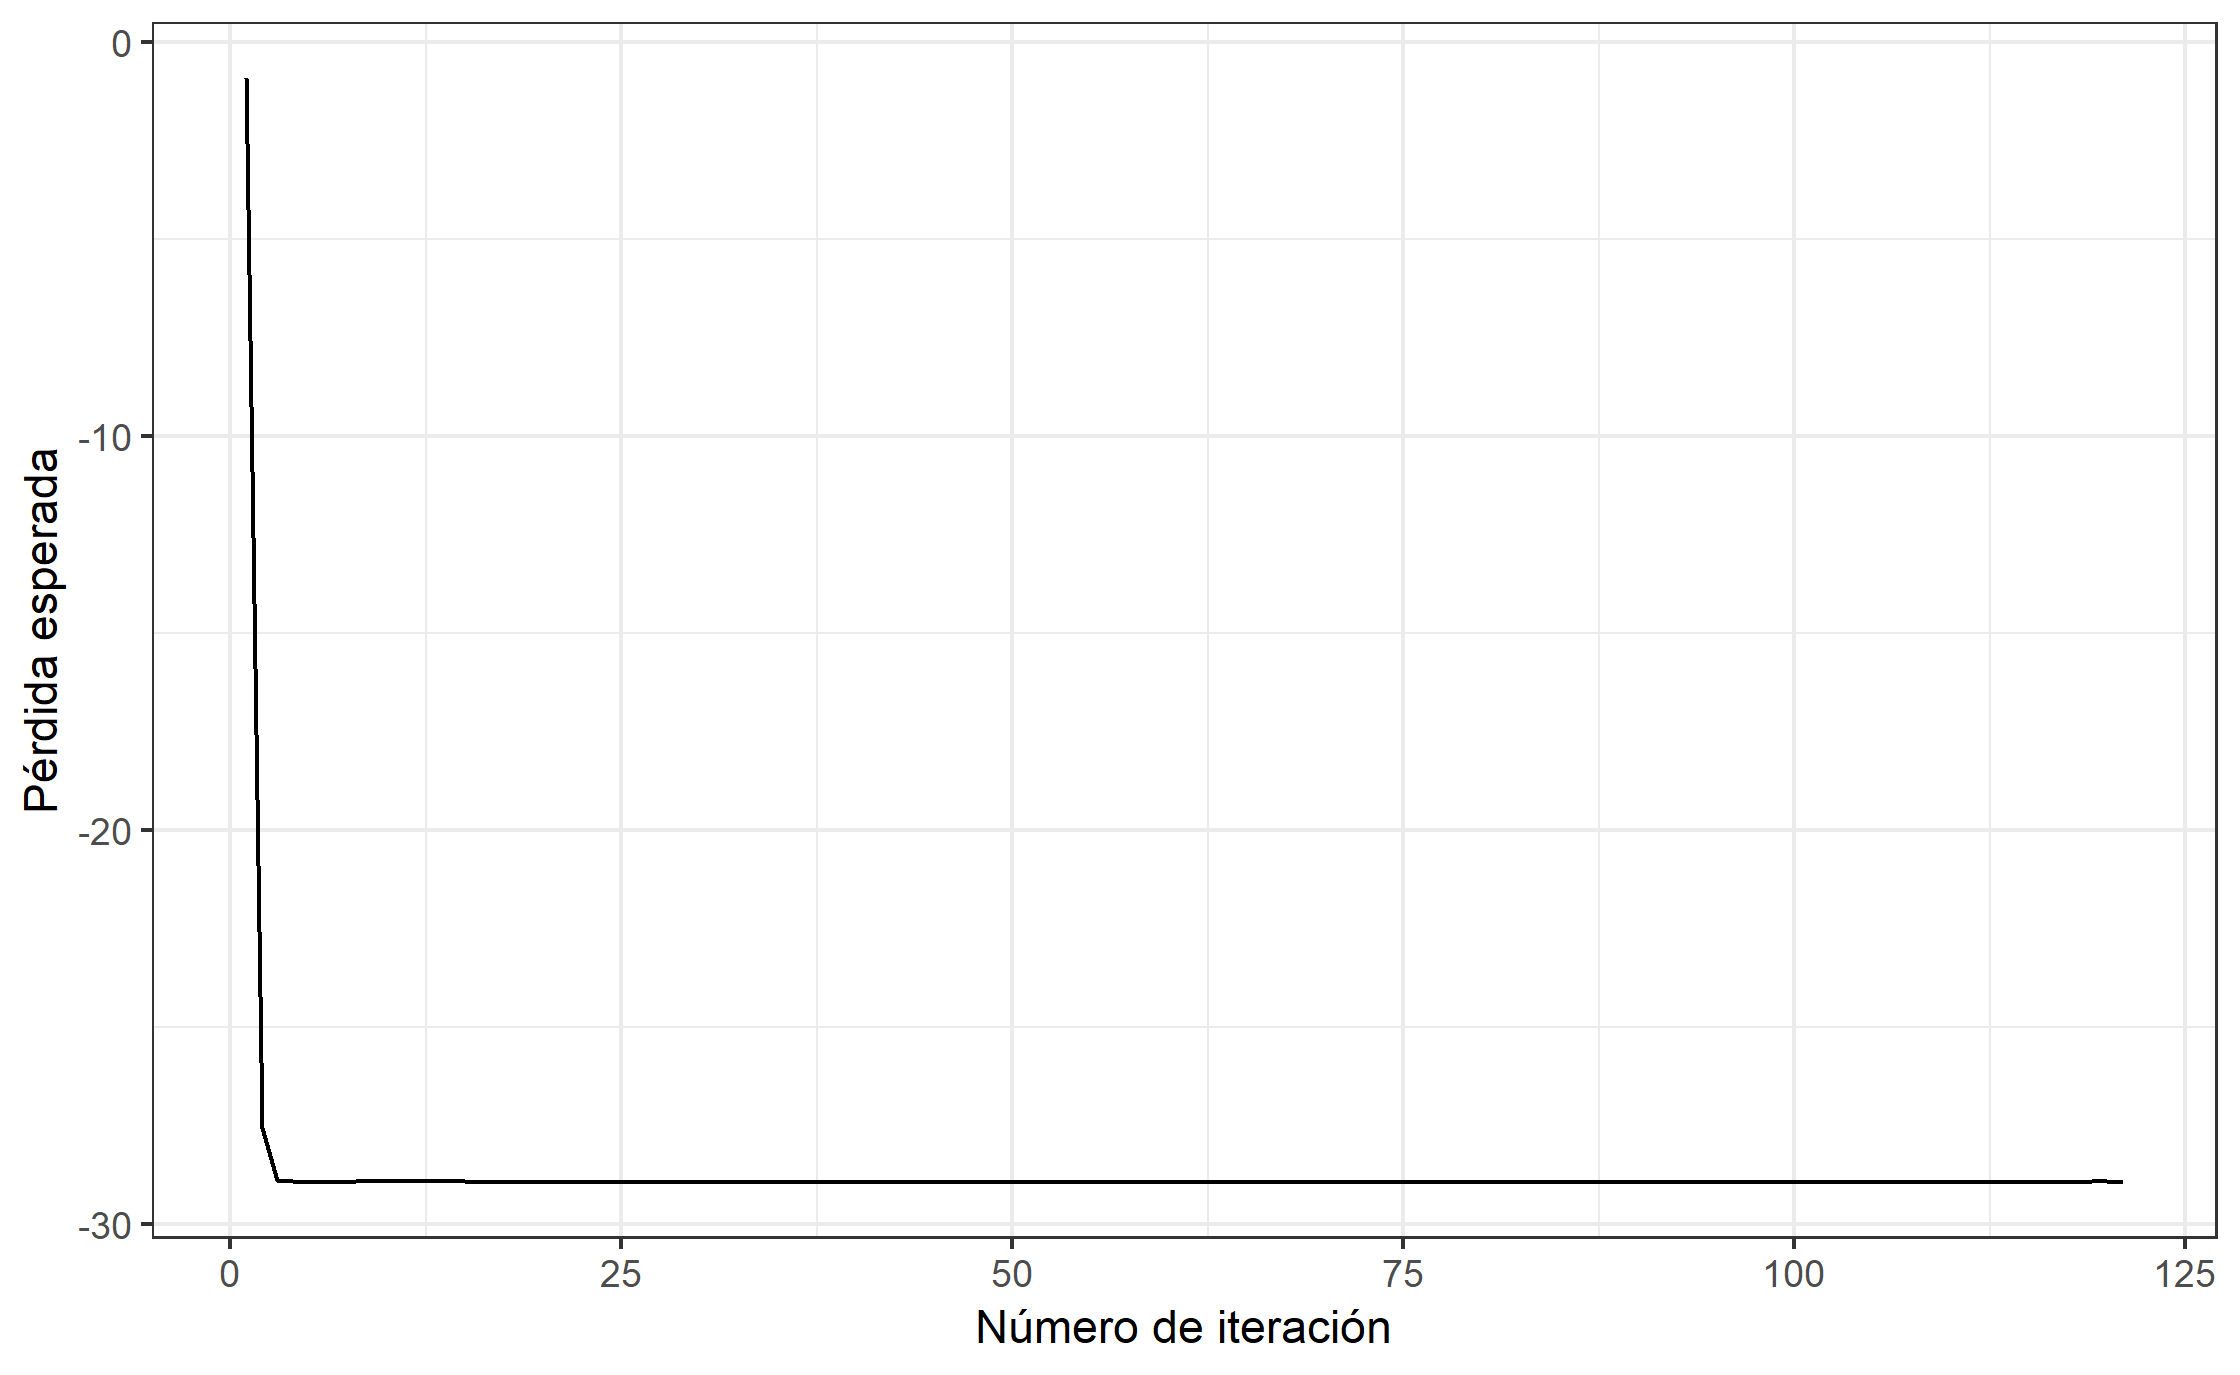
\includegraphics[width=\textwidth]{fig_conv_pois_reg_alfa5.png}
    \caption{Para la regresión Poisson con $\alpha = 0.5$, se muestran aproximaciones a la utilidad esperada de los diseños en cada iteración del algoritmo para corroborar convergencia.}
    \label{fig:pois_reg_conv_alfa5}
\end{figure}


De nuevo para corroborar la convergencia del método, las Figuras \ref{fig:pois_reg_conv_alfa5} y \ref{fig:pois_reg_conv_alfa75} muestran las aproximaciones a las utilidades esperadas del diseño en cuestión para cada iteración del algoritmo, y para $\alpha = 0.5$ y $\alpha = 0.75$, respectivamente. En ambos casos se aprecia que dichos promedios se estabilizan, por lo que se puede concluir que el método en efecto convergió.


\begin{figure}[h]
	\centering
    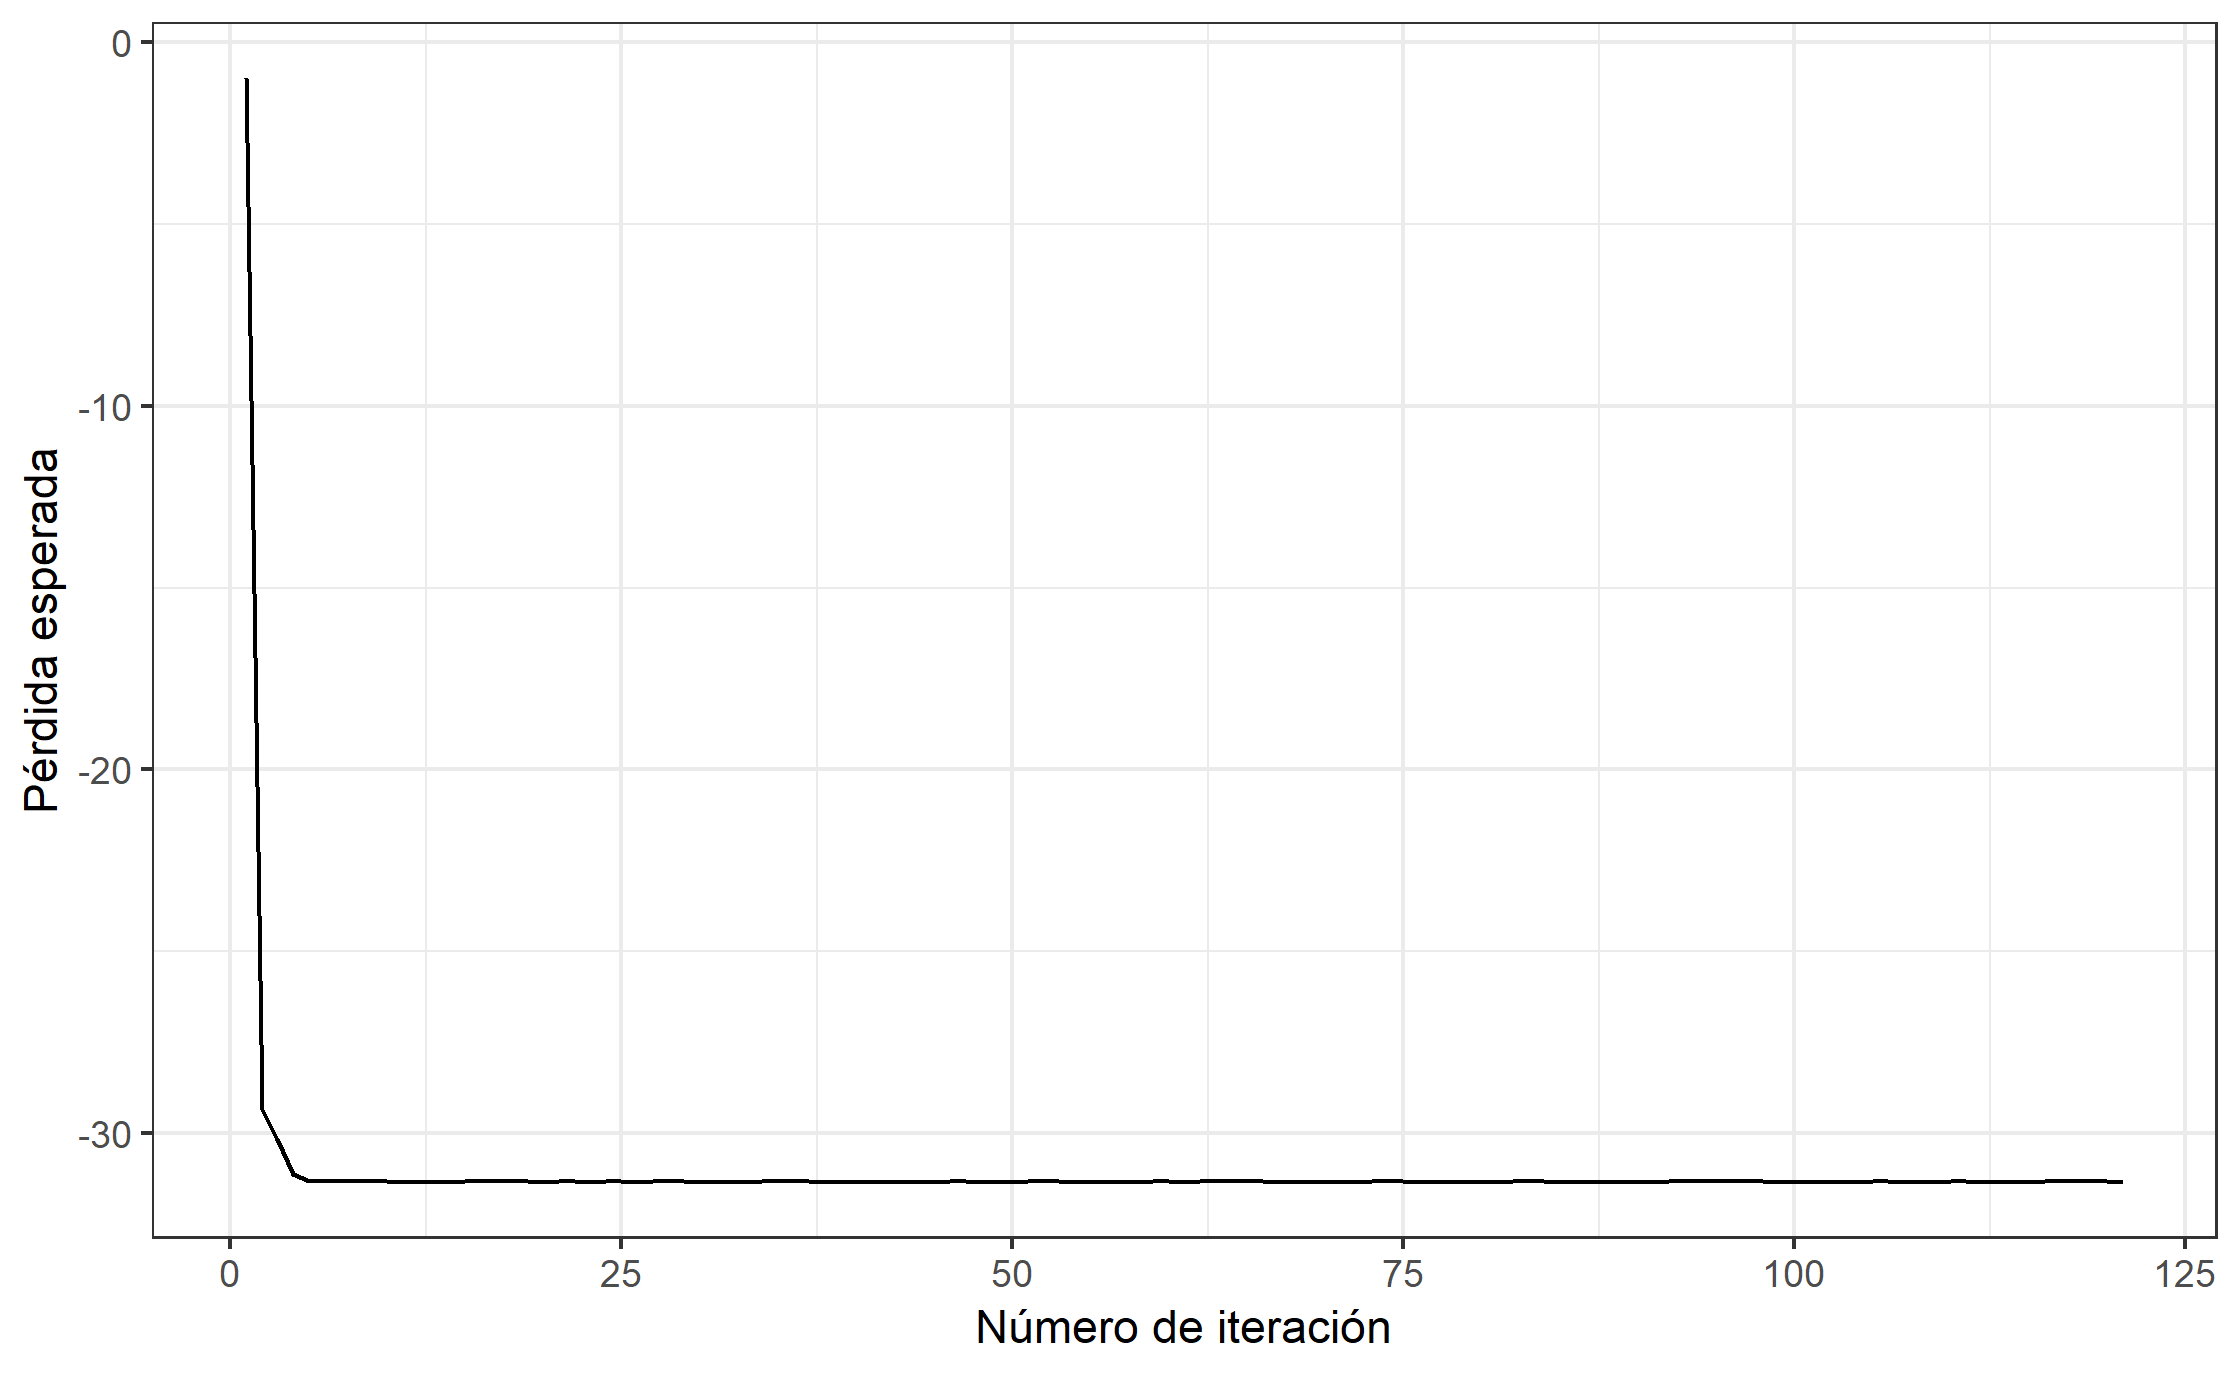
\includegraphics[width=\textwidth]{fig_conv_pois_reg_alfa75.png}
    \caption{Para la regresión Poisson con $\alpha = 0.75$, se muestran aproximaciones a la utilidad esperada de los diseños en cada iteración del algoritmo para corroborar convergencia.}
    \label{fig:pois_reg_conv_alfa75}
\end{figure}


\FloatBarrier



Otra manera de estudiar las diferencias entre los diseños $D$~-óptimos y los diseños SIL~-óptimos es comparando las distribuciones posteriores a las que dan lugar. Para ello es necesario conocer los verdaderos valores de los parámetros $\beta$, lo cual no ocurre en este caso. Sin embargo, para efectos prácticos, puede escogerse algún valor cualquiera dentro del soporte de cada parámetro y suponerlo como cierto. Aunque podría optarse por escoger la media de cada distribución, o bien la mediana o algún cuantil, para este trabajo se obtuvo una observación de cada una de las distribuciones iniciales marginales de estos parámetros; estas observaciones se fijaron y se supusieron como los valores reales de cada parámetro. Puntualmente se supuso que
\begin{align} \label{eq:beta_sim}
\begin{split}
	&\beta_1 = 1.47, \quad \beta_2 = -1.14, \quad \beta_3 = 1.24, \\
    &\beta_4 = -1.50, \quad \beta_5 = 1.41.
\end{split}
\end{align}

Es posible obtener datos simulados $y$ conjuntando los valores (\ref{eq:beta_sim}) de $\beta$ con algún diseño óptimo y utilizando la expresión del modelo (\ref{eq:mod2_poisson_regression1}). Para este ejercicio se fijó $\alpha = 0.5$ y se obtuvieron así dos series de $n=6$ datos simulados: $y_D$, correspondiente a los datos obtenidos con el diseño $D$~-óptimo, e $y_{\text{SIL}}$, correspondiente a los datos obtenidos con el diseño SIL~-óptimo. \\


Posteriormente se obtuvo, utilizando el programa \texttt{JAGS} \citep{jags}, una muestra de tamaño 10,000 de la distribución posterior de $\beta$ para cada serie de datos. La Figura \ref{fig:posterior_beta} compara las densidades marginales posteriores de cada diseño óptimo, obtenidas suavizando los datos de las muestras de cada distribución posterior. \\


Si bien las distribuciones son similares para todos los parámetros, solo en el caso de $\beta_5$ éstas son prácticamente iguales. Las distribuciones marginales posteriores de $\beta_1, \beta_2, \beta_3$, y $\beta_4$ muestran diferencias entre los diseños óptimos. \\


En el caso de $\beta_2$ y $\beta_3$ las distribuciones tienen la misma forma pero las correspondientes al diseño SIL~-óptimo están recorridas ligeramente hacia la derecha, con mayor cercanía al verdadero valor del parámetro. Las distribuciones de $\beta_1$ y $\beta_4$ son interesantes porque corresponden a valores del parámetro cercanos al extremo de su respectivo intervalo. Es notorio que las distribuciones correspondientes al diseño SIL~-óptimo tienen colas más pesadas y mayor varianza, mientras que las respectivas al diseño $D$~-óptimo están más concentradas en el extremo del intervalo.  \\



\begin{figure}[h]
	\centering
    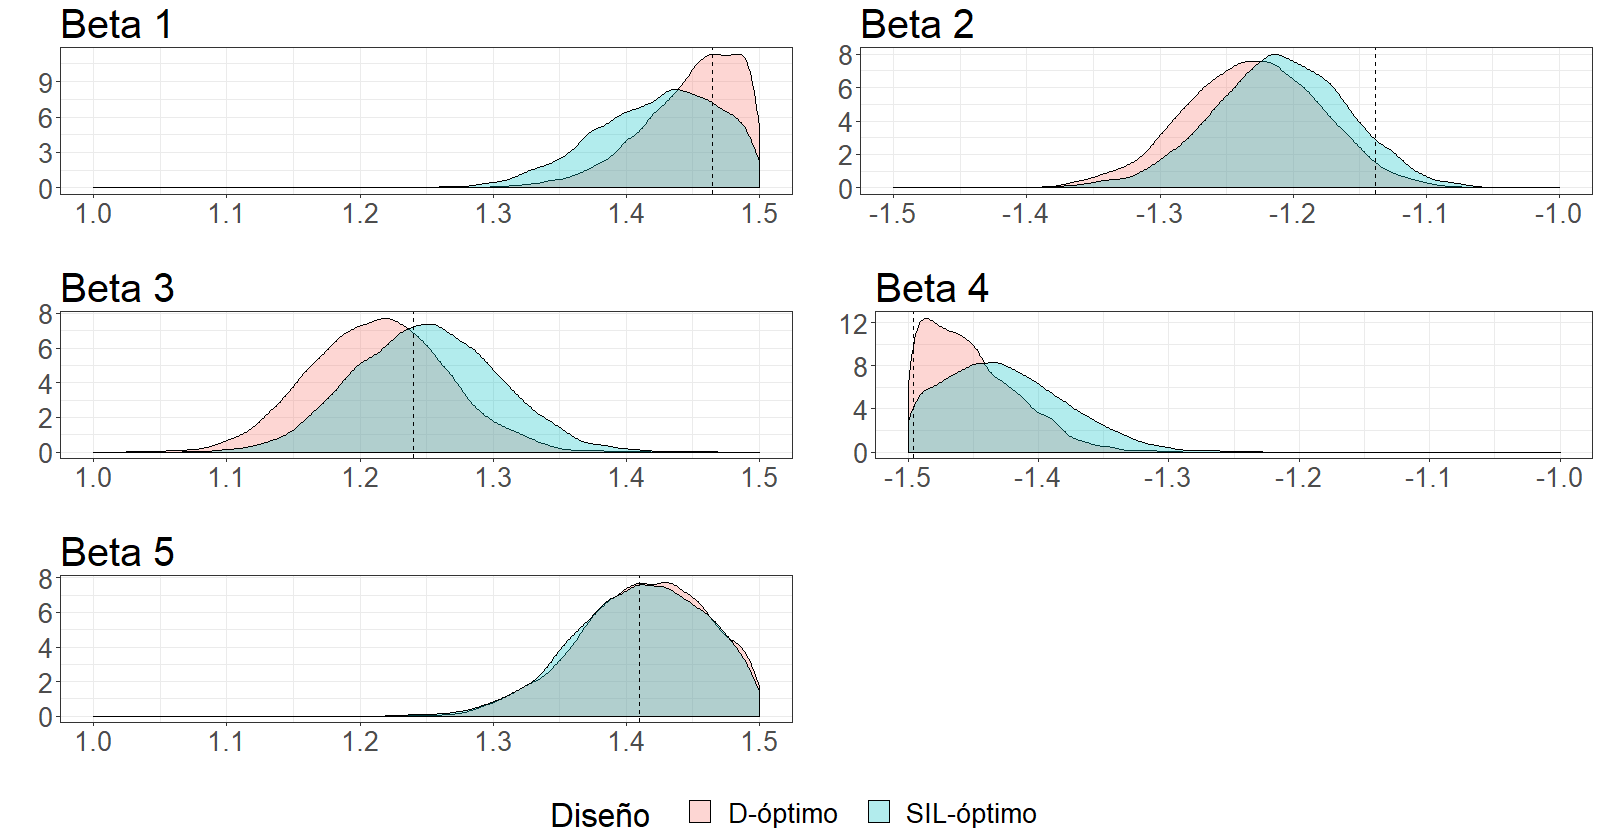
\includegraphics[width=\textwidth]{posterior_graphs_zoom.png}
    \caption{Densidades marginales posteriores de $\beta_1$, ..., $\beta_5$ derivadas de las series de datos $y_D$ e $y_{\text{SIL}}$. La línea punteada indica el valor simulado (\ref{eq:beta_sim}) del parámetro correspondiente.}
    \label{fig:posterior_beta}
\end{figure}



Por otro lado, en el ejemplo de la regresión logística las distribuciones iniciales de dos de los parámetros no contenían al cero en su soporte, ocasionando que se diera por hecho que ambos parámetros eran diferentes de cero. En este caso ocurre algo similar, solo que \textit{todos} los parámetros se suponen de dicha forma: para ambos valores de $\alpha$ (y para cualquier valor positivo de este parámetro, en realidad) las distribuciones iniciales no contienen al cero en su soporte. \\


De manera análoga al ejemplo anterior, se encontraron diseños óptimos pero habiendo modificado las distribuciones iniciales de forma que éstas sí contengan al cero en su soporte. En este caso, sin embargo, no solo se modificó el soporte de estas distribuciones, sino que además se escogió otra familia de distribuciones como sigue. Sea $\alpha > 0$ fijo. Las distribuciones iniciales propuestas por \cite{Woods_etal} (\ref{eq:mod2_params_initial}) se pueden clasificar en dos: aquellas que corresponden a $\beta_i$ con $i$ impar y aquellas que corresponden a $\beta_i$ con $i$ par. En el primer caso se considera una distribución uniforme en $(1, 1 + \alpha)$ y en el segundo una uniforme en $(-1 - \alpha, -1)$. Note que los autores suponen que todos los valores de $\beta$ son mayores que $-1 - \alpha$ y menores que $1 + \alpha$. \\


Se puede entonces pensar en una distribución inicial que, independientemente de si $i$ es par o impar, suponga que los parámetros se encuentran en el intervalo $(-1 - \alpha, 1 + \alpha)$. Además, para cambiar la familia de distribuciones y no solo el soporte, se puede utilizar alguna otra distribución que no sea uniforme. Para este propósito recordemos que la distribución Beta$(a, b)$ tiene soporte (0,1) y media igual a $a / (a + b)$. Luego, una variable aleatoria $X$ que siga una distribución Beta(2, 2) tendrá media igual a 1/2. Sea $Y = 2 (1 + \alpha) (X - \frac{1}{2})$ una transformación de la variable $X$. La función de densidad de $Y$ tiene la misma forma que la de $X$, pero con soporte igual al intervalo $(-1 - \alpha, 1 + \alpha)$. Se encontraron los diseños $D$-óptimos Bayesianos para $\alpha = 0.5$ y $\alpha = 0.75$ utilizando esta distribución como inicial para todos los parámetros. \\



Las Tablas \ref{table:alfa5_modified} y \ref{table:alfa75_modified} muestran la comparación del diseño SIL-óptimo con el $D$~-óptimo con las distribuciones iniciales modificadas y para $\alpha = 0.5$ y $\alpha = 0.75$, respectivamente. \\


\begin{table}[h]
\small
\centering
\begin{tabular}{l|lllll|lllll}
\multirow{2}{*}{Núm} & \multicolumn{5}{l|}{ \hspace{1.2cm} Diseño $D$~-óptimo} & \multicolumn{5}{l}{  \hspace{1cm}  Diseño SIL-óptimo}  \\
                     & $x_1$  & $x_2$ & $x_3$ & $x_4$ & $x_5$ & $x_1$ & $x_2$ & $x_3$ & $x_4$ & $x_5$  \\ \hline
1                    & 1  & 1    & 0.96     & -1    & 1     & -0.5  & -1    & 1     & -1    & 1      \\
2                    & 1      & 1  & 1     & 1    & -1     & 1     & 0.56  & 1     & -1    & 1      \\
3                    & -1      & -0.99    & -1  & -1    & -1     & 1     & -1    & -0.31 & -1    & 1      \\
4                    & -1      & 1    & -1     & 1  & 1     & 1     & -1    & 1     & 0.33  & 1      \\
5                    & 1      & -1    & -1     & 1    & 1 & 1     & -1    & 1     & -1    & -0.38 \\
6                    & -1      & -1    & 1     & 1    & 1     & 1     & -1    & 1     & -1    & 1     
\end{tabular}
\caption{Se muestran los diseños óptimos según los dos distintos criterios para $\alpha = 0.5$ y con las distribuciones iniciales modificadas.}
\label{table:alfa5_modified}
\end{table}



\begin{table}[h]
\small
\centering
\begin{tabular}{l|lllll|lllll}
\multirow{2}{*}{Núm} & \multicolumn{5}{l|}{ \hspace{1.2cm} Diseño $D$~-óptimo} & \multicolumn{5}{l}{  \hspace{1cm}  Diseño SIL-óptimo}  \\
                     & $x_1$  & $x_2$ & $x_3$ & $x_4$ & $x_5$ & $x_1$ & $x_2$ & $x_3$ & $x_4$ & $x_5$  \\ \hline
1                    & 1  & 1    & 1     & -1    & 1     & -0.22  & -1    & 1     & -1    & 1      \\
2                    & 1      & 1  & 1     & 1    & -1     & 1     & 0.22  & 1     & -1    & 1      \\
3                    & -1      & -1    & -1  & -1    & -1     & 1     & -1    & -0.32 & -1    & 1      \\
4                    & -1      & 1    & -1     & 1  & 1     & 1     & -1    & 1     & 0.11  & 1      \\
5                    & 1      & -1    & -1     & 1    & 1 & 1     & -1    & 1     & -1    & -0.31 \\
6                    & -1      & -1    & 1     & 1    & 1     & 1     & -1    & 1     & -1    & 1     
\end{tabular}
\caption{Se muestran los diseños óptimos según los dos distintos criterios para $\alpha = 0.75$ y con las distribuciones iniciales modificadas.}
\label{table:alfa75_modified}
\end{table}


Es evidente que los diseños óptimos bajo las nuevas distribuciones iniciales son diferentes a los diseños óptimos originalmente encontrados por \cite{Woods_etal} (y también a los diseños óptimos previamente encontrados). Primeramente, independientemente del valor de $\alpha$, ya no ocurre que todos los elementos de la matriz de diseño sean $\pm 1$ exceptuando a los elementos de la diagonal. Más aún, en el diseño con las iniciales originales todos los valores de cada covariable (cada columna) siempre valían lo mismo, excepto en un ensayo. En el caso de las iniciales modificadas lo que ocurre es que \textit{(i)} los elementos de la diagonal también valen $\pm 1$ y \textit{(ii)} las covariables ya no solo toman un valor (sin contar el valor de la diagonal que era distinto), sino que ahora valen 1 en algunos ensayos y -1 en otros. \\

Por otro lado al cambiar de $\alpha = 0.5$ a $\alpha = 0.75$ los diseños con las iniciales modificadas quedaron prácticamente iguales, salvo en dos entradas que son \textit{prácticamente} $\pm 1$. En resumen, la modificación de distribuciones iniciales introdujo cambios considerables en los diseño óptimos. \\


Por su parte, las Figuras \ref{fig:pois_reg5_modified} y \ref{fig:pois_reg75_modified} muestran las proyecciones en una y dos dimensiones de los diseños óptimos para $\alpha = 0.5$ y $\alpha = 0.75$, respectivamente (suavizando con un kernel Gaussiano para obtener la densidad de la proyección unidimensional).  \\

Algo interesante es que las correlaciones entre las covariables también cambiaron: si bien antes eran $\pm 0.2$ ahora no es así. En el caso de $\alpha = 0.5$ algunas correlaciones parecen estar alrededor de 1/3, otras alrededor de 0 y una última igual a 1/4. Esto se repite para el caso de $\alpha = 0.75$, donde además las correlaciones ya no están alrededor de estos valores sino que directamente eso valen. Puntualmente las correlaciones entre $x_1, x_2$ y $x_3$ son iguales a 1/3 y las respectivas a $x_4$ y $x_5$ con las demás covariables son 0, excepto precisamente por la correlación entre estas dos covariables, la cual toma el valor de 1/4. En resumen, pareciera que las covariables se separaron en dos grupos: $x_1, x_2$ y $x_3$ en un lado, correlacionadas entre sí por 1/3 pero no correlacionadas con las últimas dos covariables; y por otro lado $x_4$ y $x_5$, correlacionadas entre sí por 1/4 pero no correlacionadas con las primeras tres covariables.  \\



Finalmente las Figuras \ref{fig:pois_reg_conv_alfa5_modified} y \ref{fig:pois_reg_conv_alfa75_modified} muestran la evolución de la estimación de la pérdida esperada conforme el número de iteración avanza, para ambos valores de $\alpha$ respectivamente. En ambos casos la pérdida esperada parece haber convergido, por lo que se concluye lo mismo del método.




\begin{figure}[h]
	\centering
    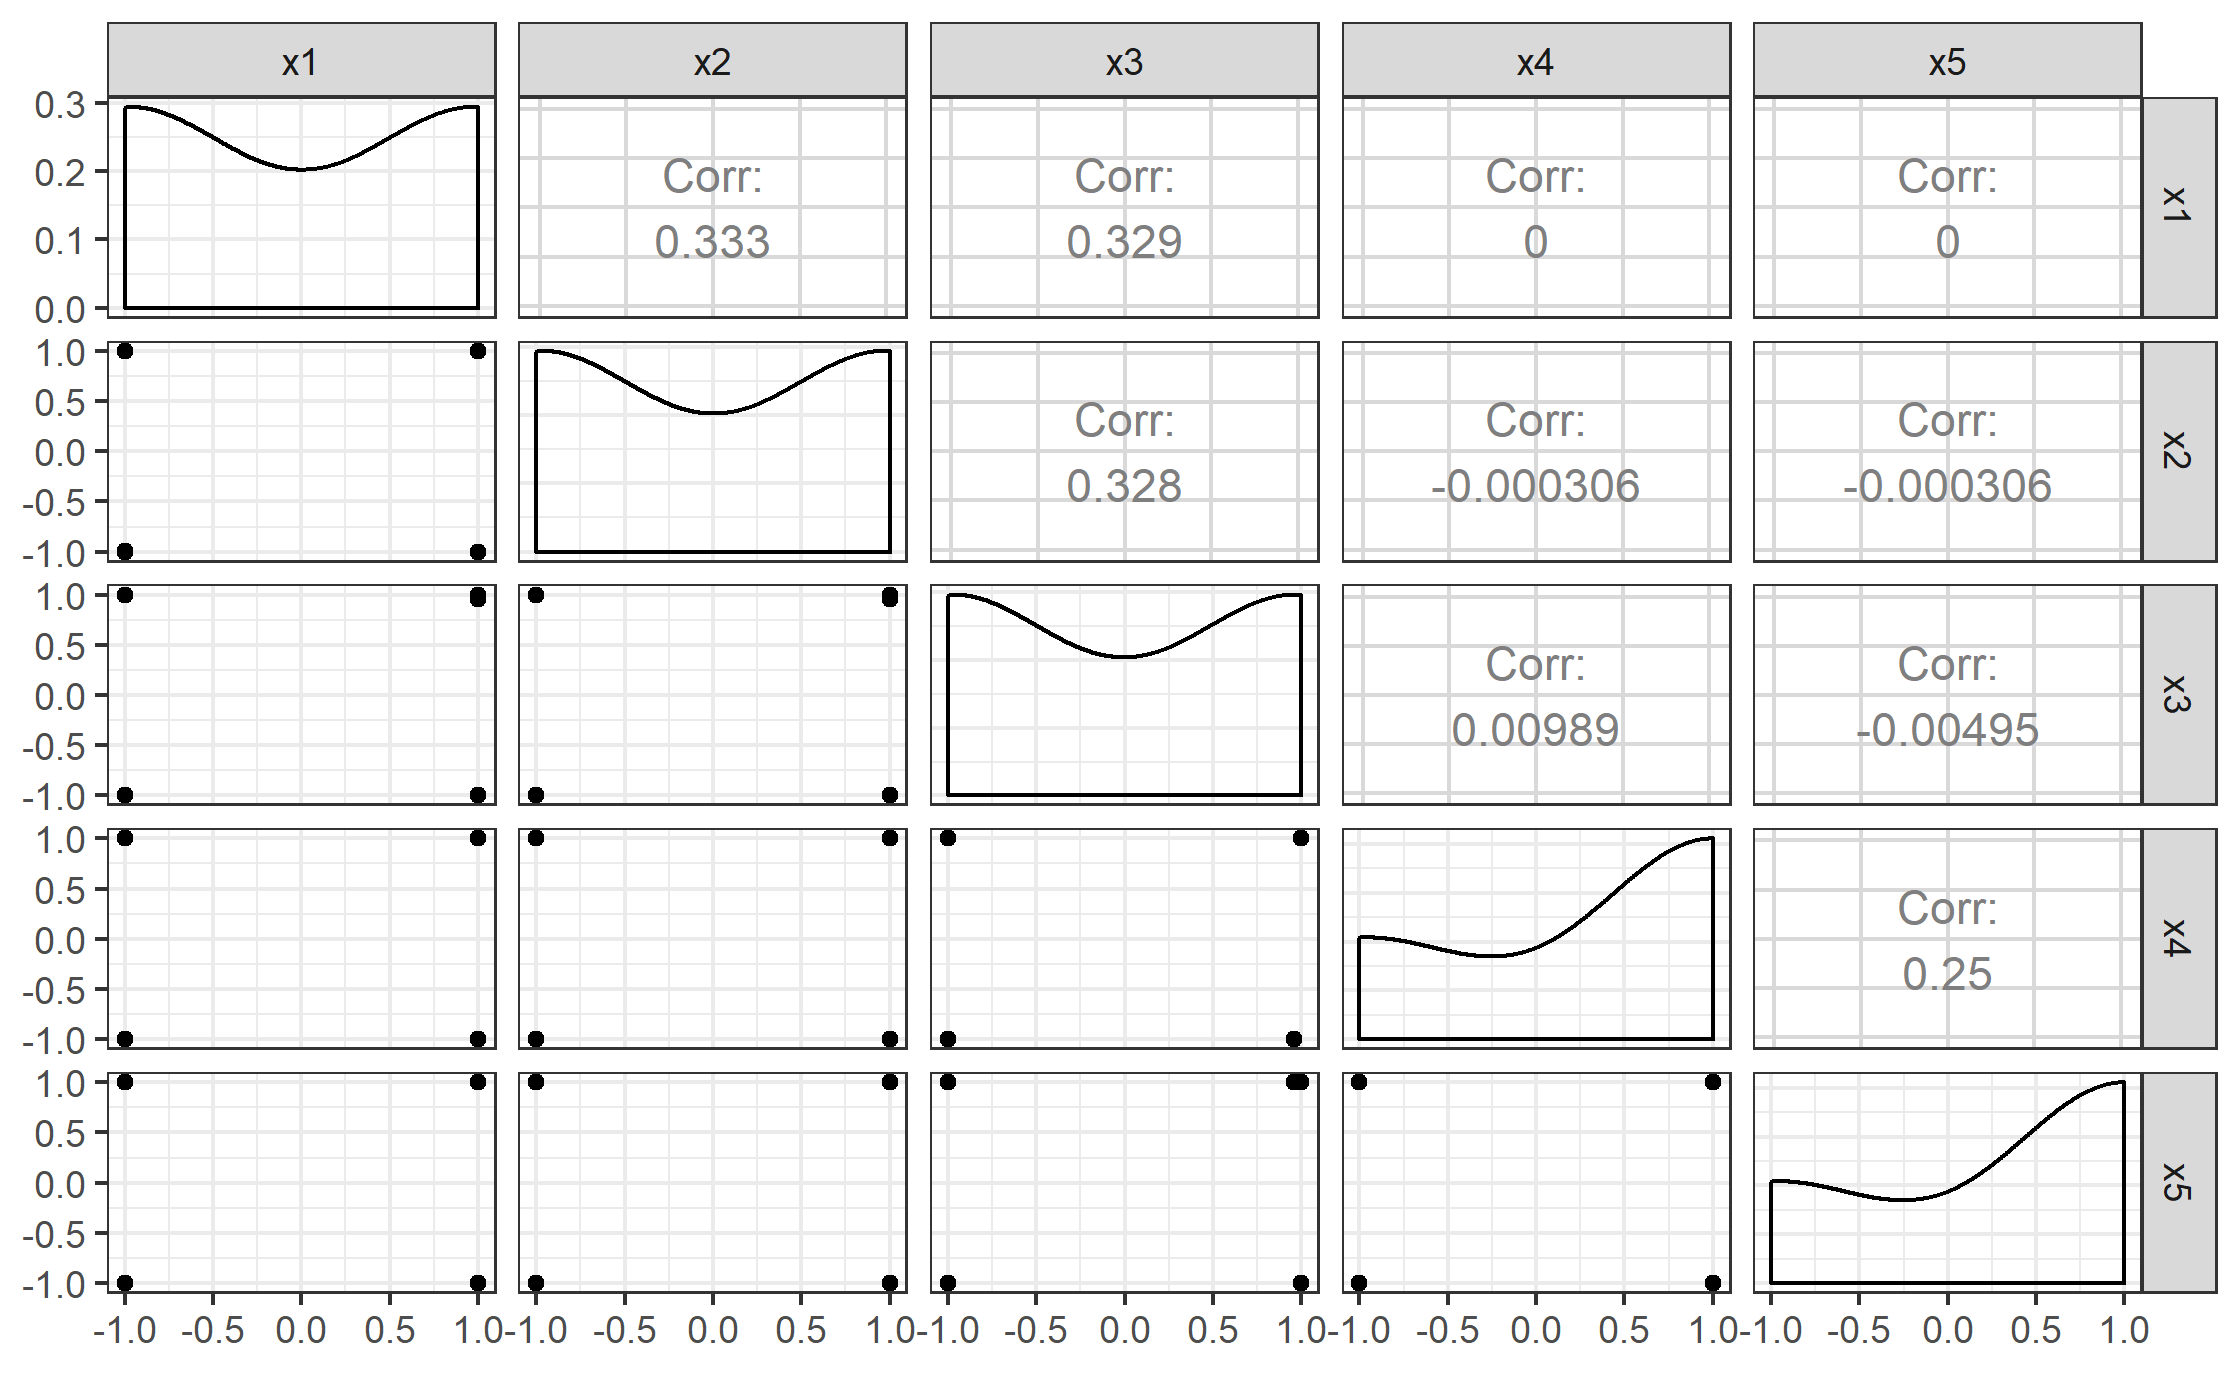
\includegraphics[width=\textwidth]{alpha_50_modified.png}
    \caption{Se muestran proyecciones en una y dos dimensiones de las tres variables del modelo de regresión Poisson (\ref{eq:mod2_poisson_regression1}) con distribuciones iniciales modificadas, así como su correlación, para $\alpha=0.5$.}
    \label{fig:pois_reg5_modified}
\end{figure}



\begin{figure}[h]
	\centering
    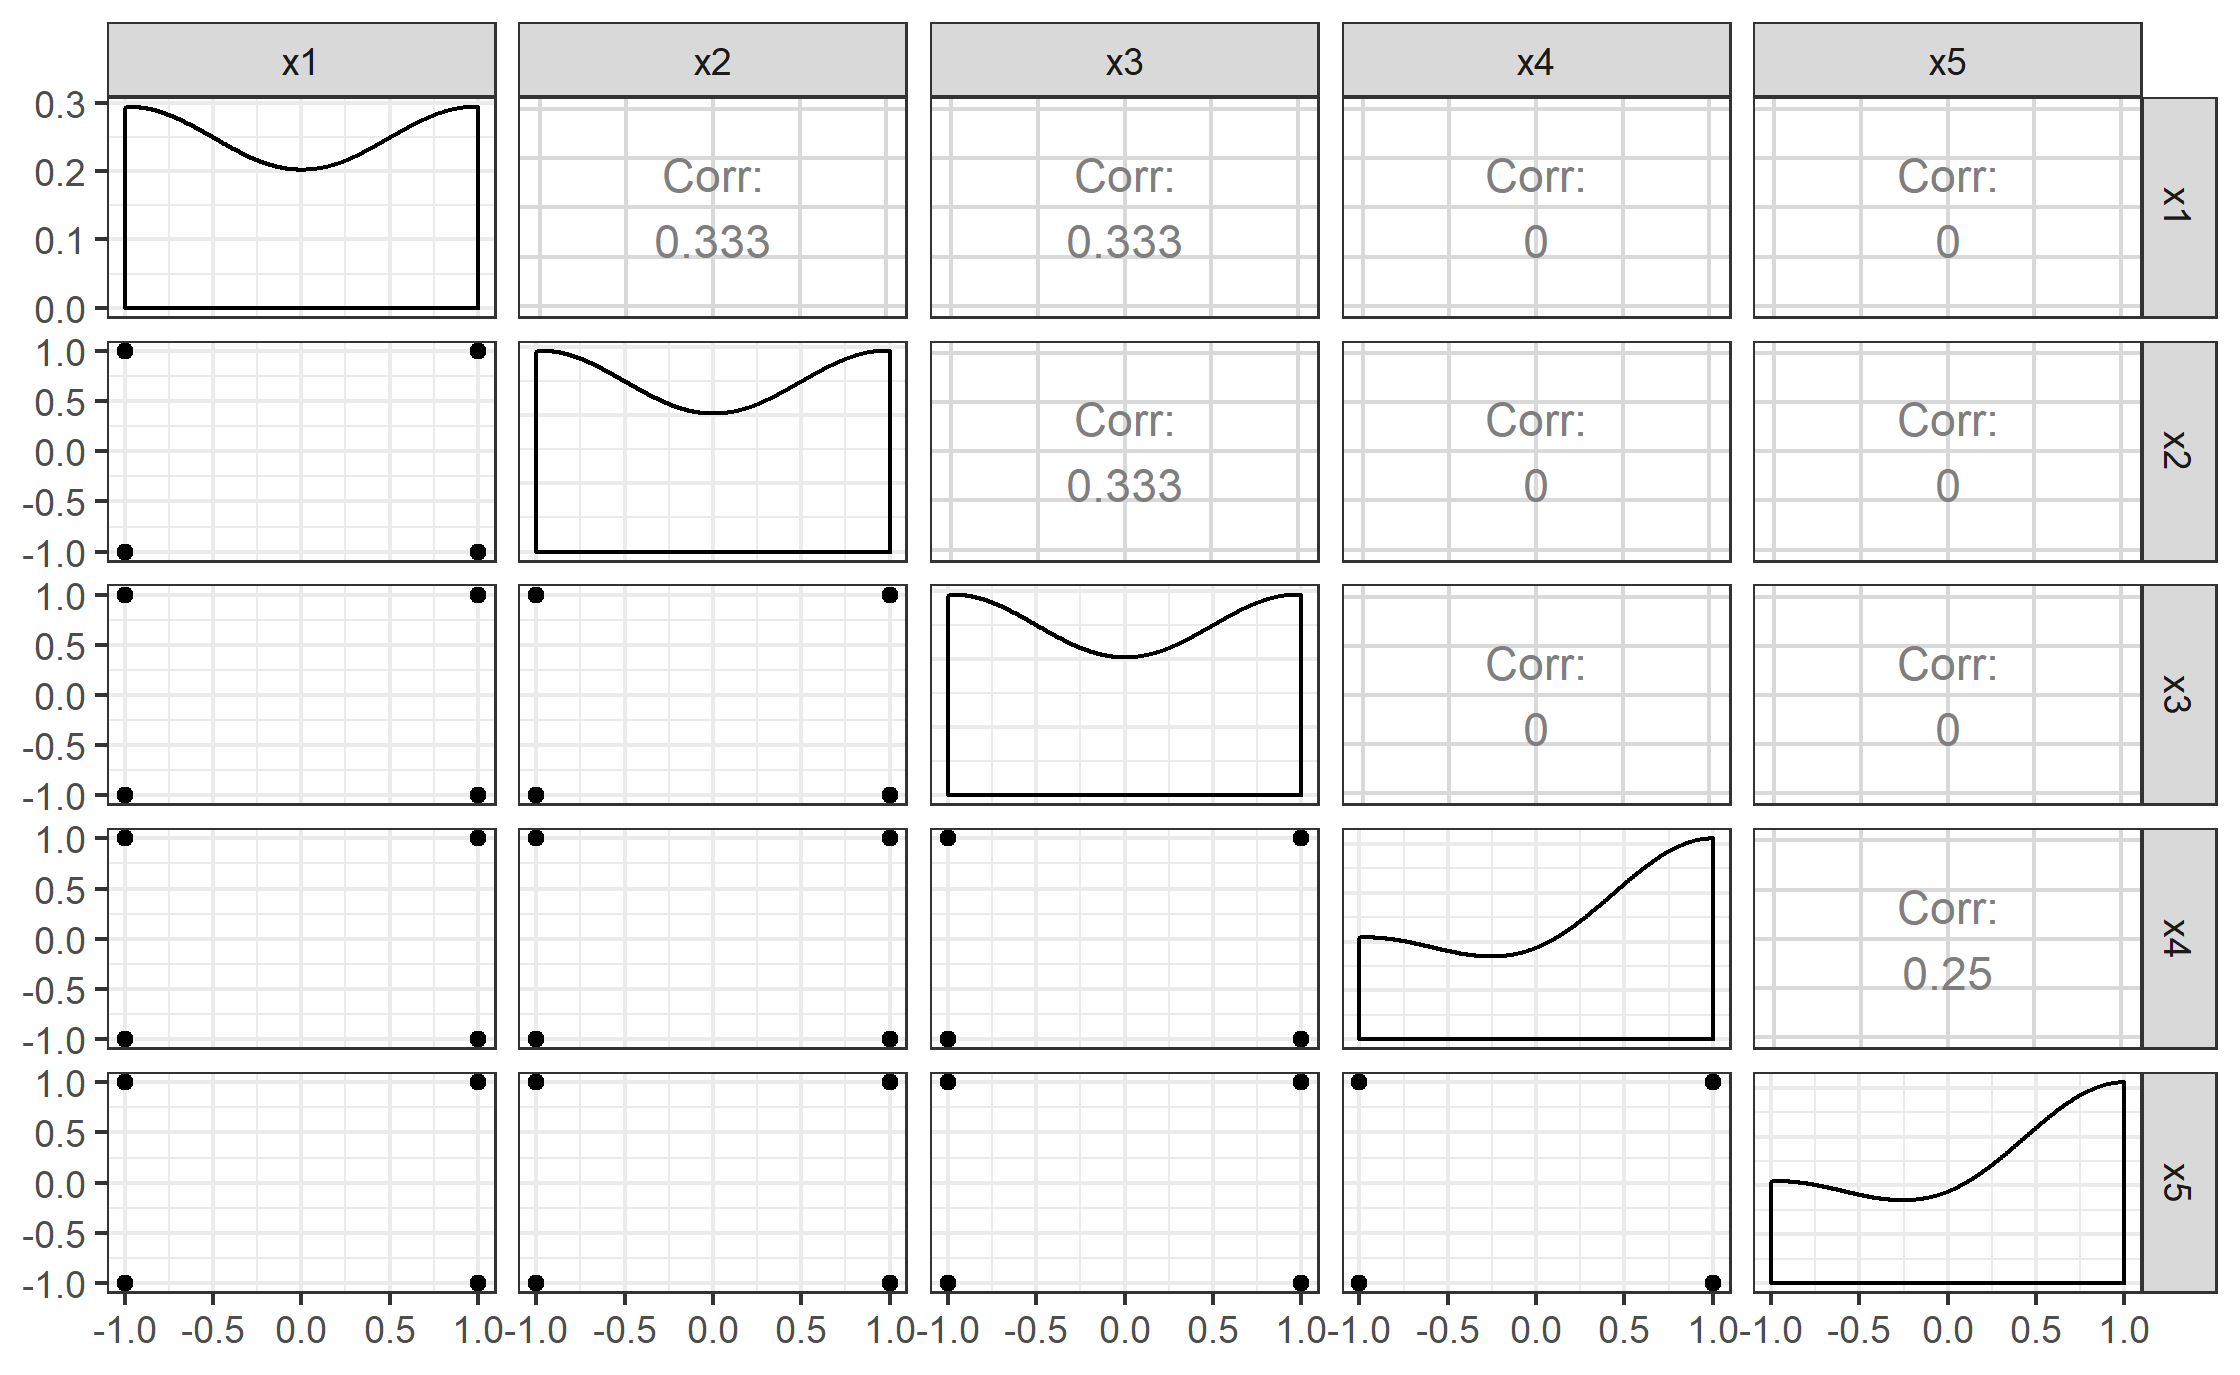
\includegraphics[width=\textwidth]{alpha_75_modified.png}
    \caption{Se muestran proyecciones en una y dos dimensiones de las tres variables del modelo de regresión Poisson (\ref{eq:mod2_poisson_regression1}) con distribuciones iniciales modificadas, así como su correlación, para $\alpha=0.75$.}
    \label{fig:pois_reg75_modified}
\end{figure}








\begin{figure}[h]
	\centering
    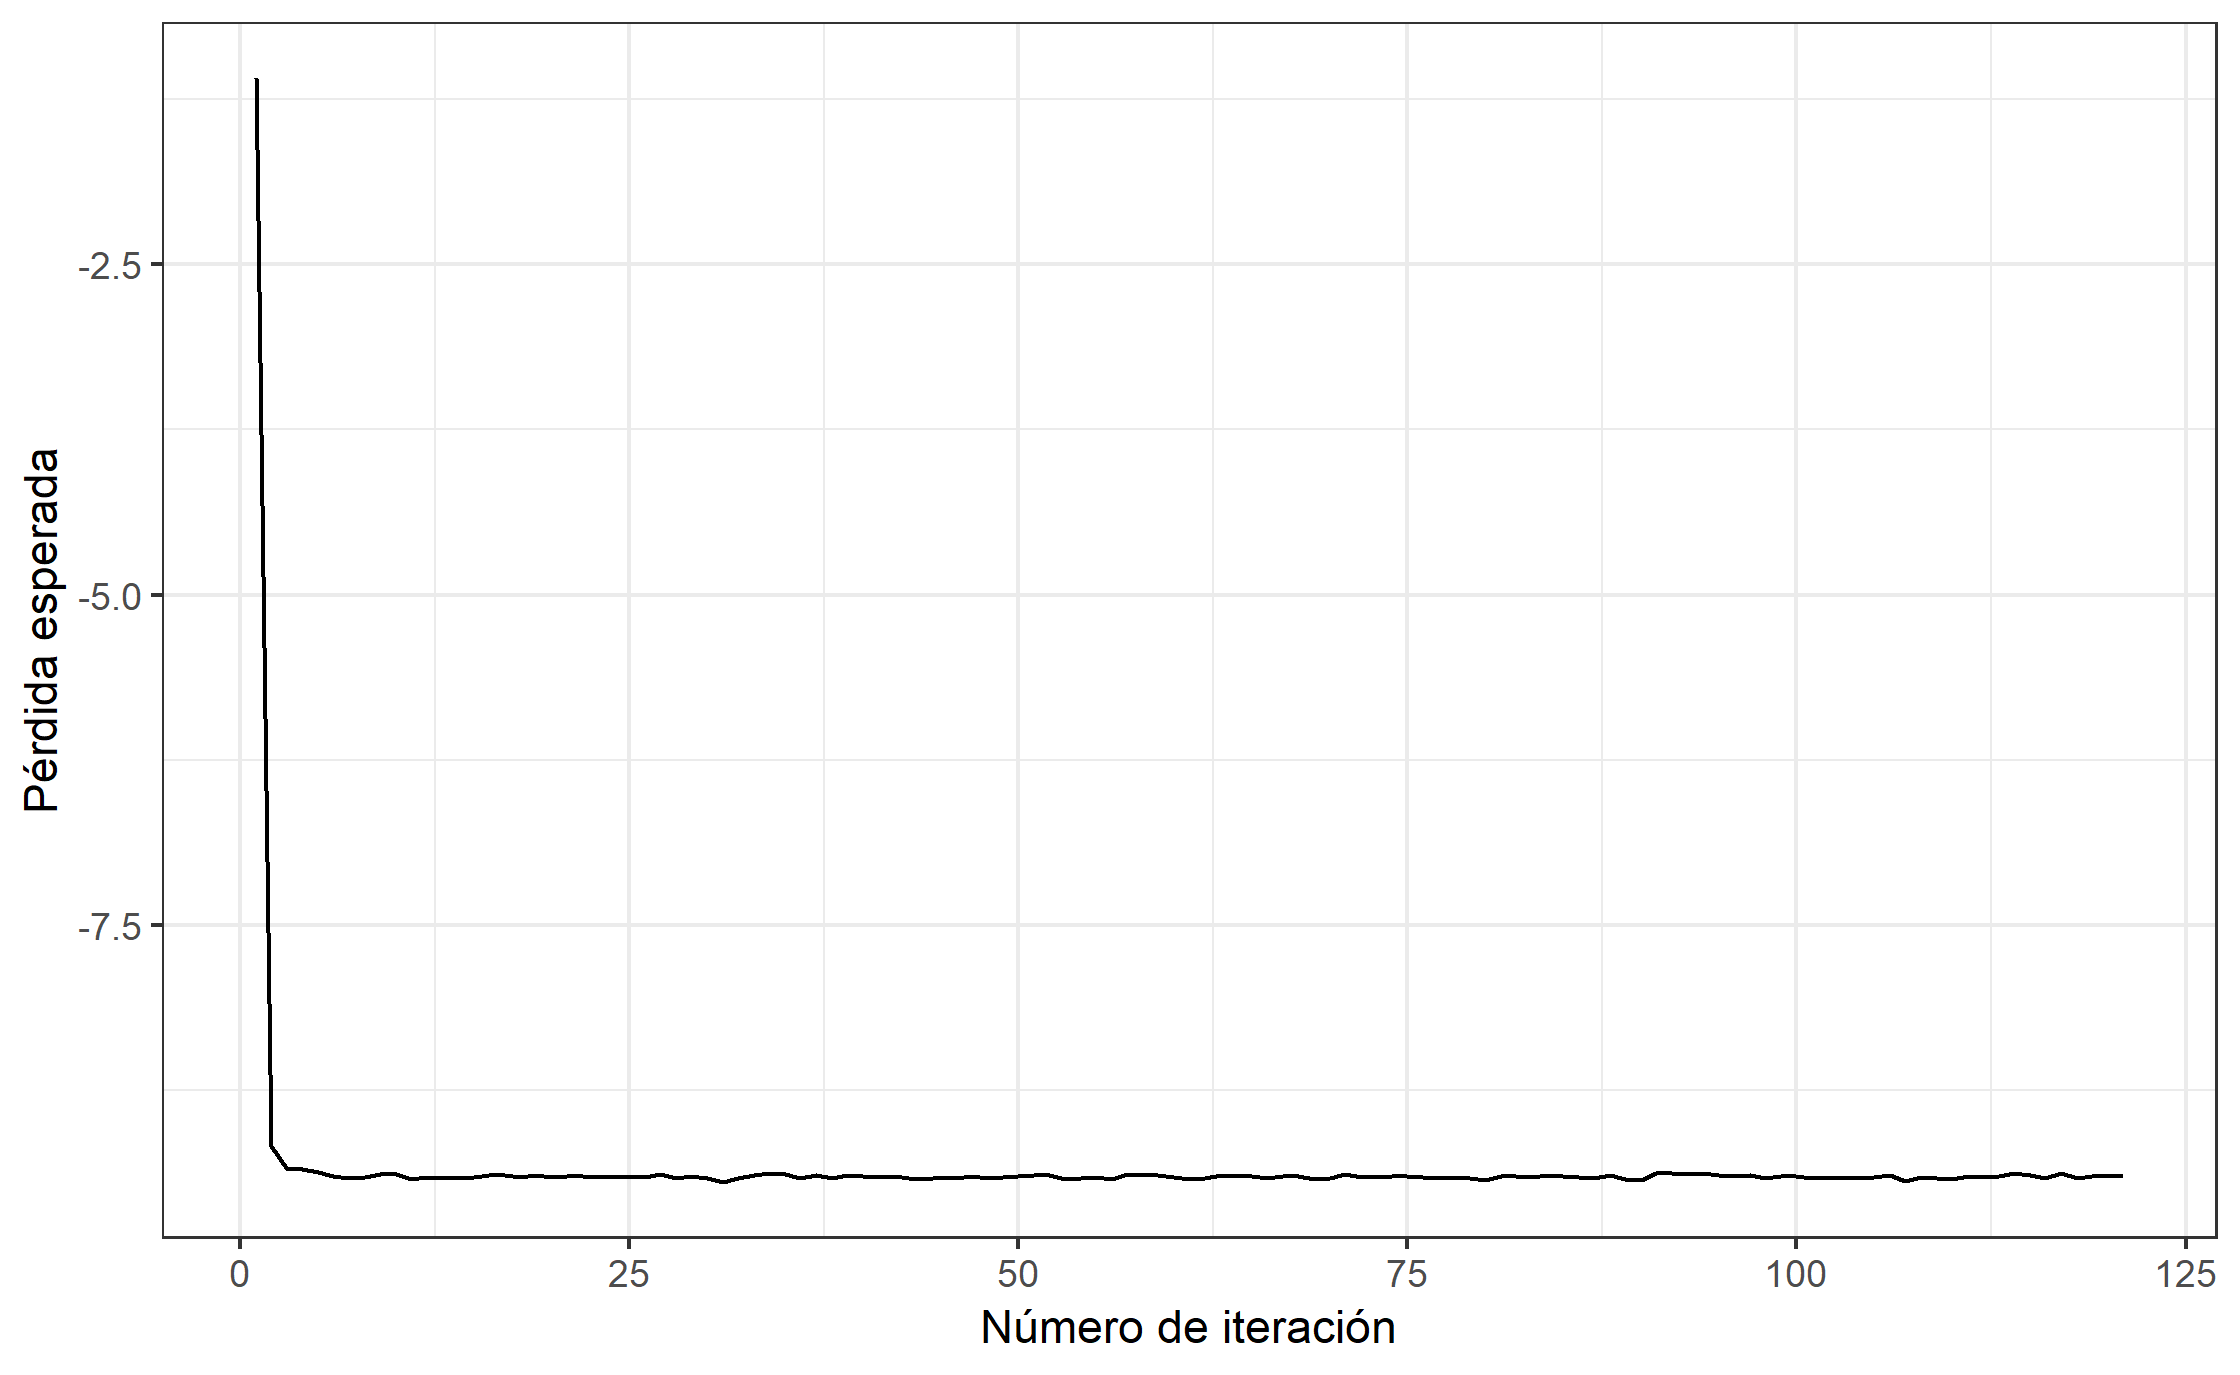
\includegraphics[width=\textwidth]{fig_conv_pois_reg_alfa5_modified.png}
    \caption{Para la regresión Poisson con distribuciones iniciales modificadas y $\alpha = 0.5$, se muestran aproximaciones a la utilidad esperada de los diseños en cada iteración del algoritmo para corroborar convergencia.}
    \label{fig:pois_reg_conv_alfa5_modified}
\end{figure}



\begin{figure}[h]
	\centering
    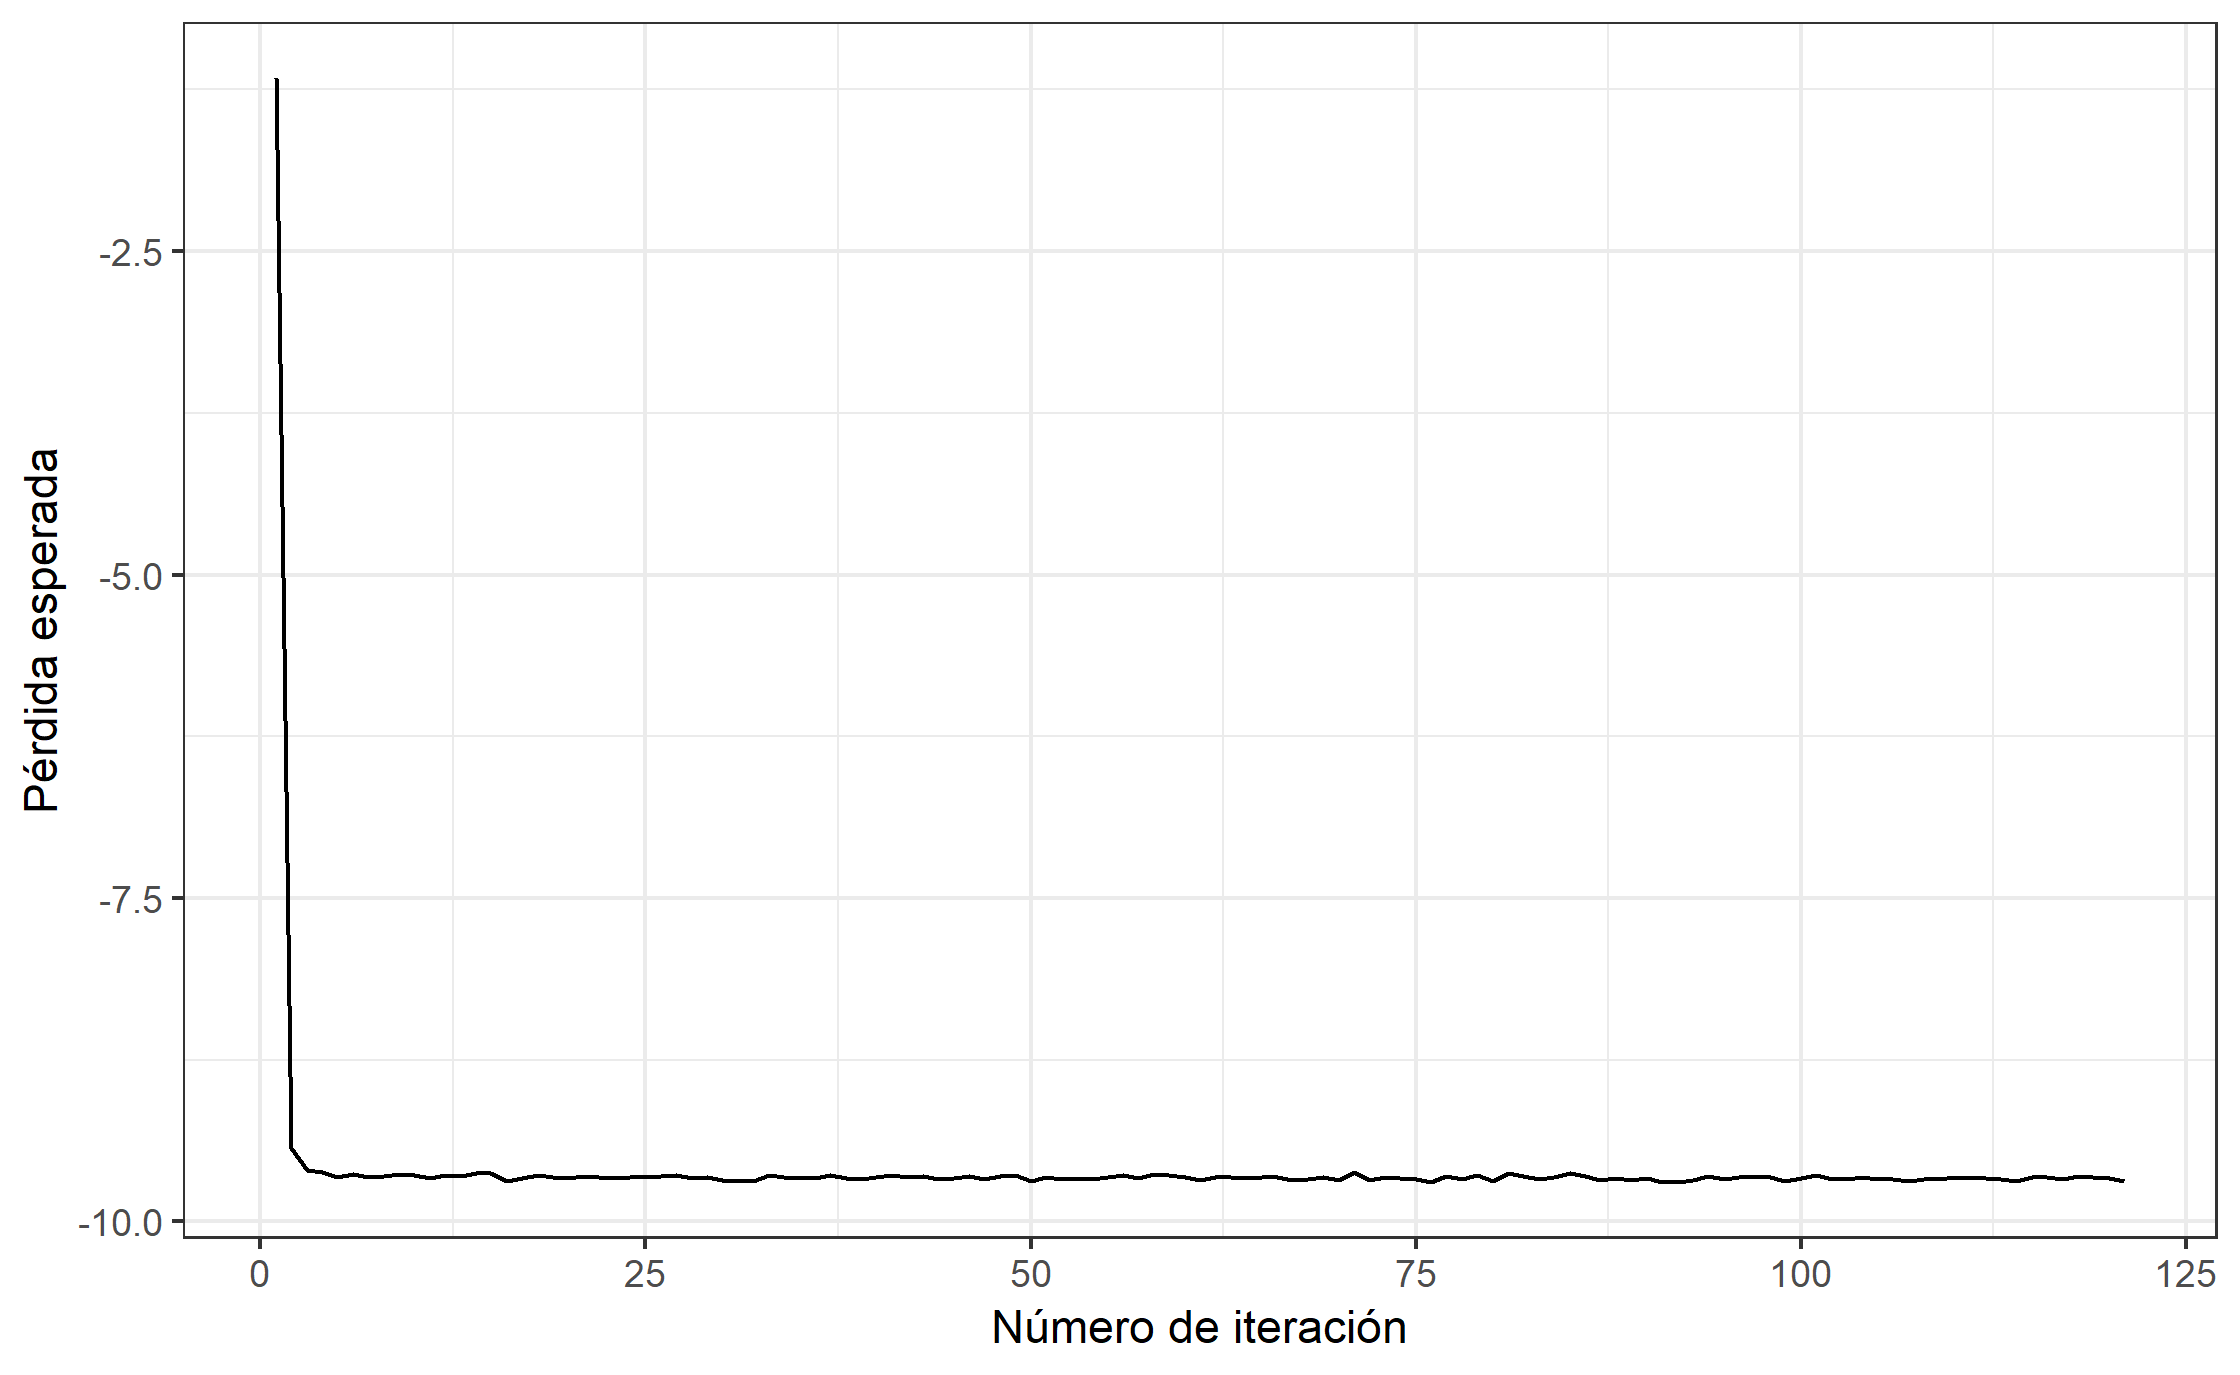
\includegraphics[width=\textwidth]{fig_conv_pois_reg_alfa75_modified.png}
    \caption{Para la regresión Poisson con distribuciones iniciales modificadas y $\alpha = 0.75$, se muestran aproximaciones a la utilidad esperada de los diseños en cada iteración del algoritmo para corroborar convergencia.}
    \label{fig:pois_reg_conv_alfa75_modified}
\end{figure}




\FloatBarrier






En el Apéndice \ref{chapter:appendixCode} se incluye el código utilizado para encontrar los diseños óptimos para cada uno de los ejemplos, así como para generar las gráficas aquí mostradas.










%\begin{figure}[h]
%\centering
%\begin{subfigure}{0.5\textwidth}
%  \centering
%  \includegraphics[scale=0.28]{pois_reg_alfa0_5}
%  \caption{$\alpha=0.5$.}
%  \label{fig:alfa.5}
%\end{subfigure}%
%\begin{subfigure}{0.5\textwidth}
%  \centering
%  \includegraphics[scale=0.28]{pois_reg_alfa0_75}
%  \caption{$\alpha=0.75$.}
%  \label{fig:alfa.75}
%\end{subfigure}
%\caption{Se muestran las proyecciones en una y dos dimensiones de las cinco %variables del modelo de regresión Poisson (\ref{eq:mod2_poisson_regression1}), así como su correlación, para los casos $\alpha = 0.5$ y $\alpha = 0.75$.}
%\label{fig:pois_reg}
%\end{figure}


%\section{Diseño para modelo de regresión Gamma}


%La distribución Gamma tiene la propiedad de ser sesgada a la derecha. Esto la hace sumamente útil para modelar fenómenos que sean no negativos y concentrados en una cierta región, pero que también produzcan datos atípicos. Uno puede pensar, por ejemplo, en el tiempo hasta que algún evento ocurra. Es en parte por ello que la distribución Gamma es popular en la práctica. En particular, es posible modelar respuestas que sigan dicha distribución mediante un modelo lineal generalizado. Como se menciona en el Apéndice \ref{chapter:appendixGLMs}, uno de los problemas es que la liga canónica es poco útil. La alternativa más popular, la liga logarítmica, ha dado buenos resultados y es bastante popular en la literatura. \\










\chapter{Conclusiones} \label{chapter:conclusiones}

\epigraph{\textit{The concept of the statistician as one who analyzes someone else's data is flawed, but equally inaproppiate is the idea of the statistician engaged only in the design and analysis of an individual experiment.}}{--- Box y Liu, \textit{Statistics as a Catalyst to Learning by Scientific Method Part I--An Example} (1999)}




La importancia del diseño de experimentos radica en que éste permite que la recolección de datos se realice acorde a algún criterio de optimalidad, el cual debe reflejar el objetivo final del estudio en cuestión. Esto eleva la calidad de cualquier análisis inferencial hecho con base en los datos, pues permite que quien realiza el experimento modifique las covariables y observe el valor resultante de la variable respuesta en un ambiente controlado. \\




El problema de diseño experimental se puede plantear de manera natural como un problema de decisión, lo cual lo coloca en el marco de la Estadística Bayesiana. Sin embargo inmediatamente aparecen complicaciones en la formulación; en particular en la mayoría de los casos no existen soluciones analíticas. Más aún, dichas soluciones son difíciles de encontrar incluso mediante métodos computacionales. Una estrategia que ha resultado de utilidad es suponer conocido el modelo de muestreo de la variable respuesta, pues esto puede simplificar algunos de los cálculos numéricos. Los modelos lineales generalizados son de gran ventaja en este caso, pues son lo suficientemente generales como para que muchos fenómenos se puedan modelar con ellos pero a la vez han sido estudiados con profundidad en la literatura. \\




El método ACE es uno de los algoritmos más recientes para encontrar diseños óptimos \citep{Woods_ACE}, y es particularmente útil en el marco de modelos lineales generalizados y criterios de optimalidad Bayesiana populares. En esta tesis se utilizó este método para abordar dos problemas de diseño de experimentos para modelos lineales generalizados: una regresión logística y una regresión Poisson. Ambos provienen de un artículo publicado por \cite{Woods_etal}, en donde los autores muestran distintas aplicaciones del método ACE. \\




En el caso de la regresión logística el diseño encontrado fue consistente con el encontrado por Woods et al. Para la regresión Poisson se encontraron diseños óptimos utilizando un criterio de optimalidad distinto al propuesto por los autores, lo que implicó consecuencias interesantes en las que se ahondará más adelante. Por otra parte se discutió el hecho de que, en ambos ejemplos, Woods et al. utilizaron distribuciones iniciales que presuponían a los parámetros del modelo como diferentes de cero. Por ello se obtuvieron diseños óptimos con distribuciones iniciales modificadas que evitaran este supuesto. \\




No está de más recordar que, en el ejemplo de la regresión logística, se ilustró la dificultad que se encuentra al buscar una expresión analítica para la pérdida esperada. En el camino se resaltó la complejidad inherente a los cálculos relacionados con la optimización de la pérdida esperada. Este ejemplo ilustra por qué es necesario, en muchos casos, recurrir a métodos computacionales que asistan con la obtención del diseño óptimo. Por otra parte, al modificar el soporte de las distribuciones iniciales de forma que éste contuviera al cero, se encontró un diseño óptimo diferente al original. Puntualmente se observó que las únicas covariables afectadas eran las correspondientes a los parámetros cuyas distribuciones iniciales marginales fueron modificadas, y en ese caso ocurrió que la correlación entre estas covariables disminuyó considerablemente en el nuevo diseño óptimo. \\


El ejemplo de la regresión Poisson fue exhaustivo y dio lugar a algunos hallazgos que merecen mayor discusión. En primer lugar el hecho de utilizar criterios de optimalidad distintos derivó en diseños óptimos diferentes. Más aún, la distribución final del parámetro a la que cada diseño dio lugar difirió según el criterio de optimalidad empleado. Por otro lado se modificó la distribución inicial del parámetro. A diferencia del ejemplo de la regresión logística, en este caso se cambió tanto el espacio parametral como la forma de la distribución inicial. Ello derivó en diseños óptimos radicalmente distintos de los originalmente encontrados. Los diseños modificados no mostraban el patrón visto en los originales, es decir, columnas constantes (e iguales a $\pm 1$) salvo en una entrada, sino que contenían combinaciones de $\pm 1$ en todas sus entradas. \\



De estos dos ejemplos se concluye que tanto el criterio de optimalidad como la distribución inicial del parámetro son elementos de suma importancia y que pueden tener un impacto considerable en el diseño óptimo encontrado, además de que se resaltó la necesidad de emplear métodos computacionales debido a la complejidad analítica del diseño Bayesiano de experimentos. \\



%En primer lugar el diseño óptimo encontrado varía tanto si solo se cambia el criterio de optimalidad como si además se modifican las distribuciones iniciales. Esto resalta por un lado la importancia de la función de pérdida o utilidad, que da lugar a los criterios de optimalidad. Ésta se debe de escoger de manera que los objetivos del experimento se vean reflejados en ella, y no hacerlo puede acarrear consecuencias negativas para el estudio. Por otro lado se concluye que la manera en la que se reflejan los conocimientos iniciales tiene un impacto en el resultado del análisis, por lo que es imperativo que quien realiza el estudio cuestione cuál es y cómo representar la información inicial que tiene acerca del fenómeno de estudio. \\




%En segundo lugar si bien los diseños óptimos son distintos estos contienen similitudes importantes. En todos los casos todas las covariables tomaban el mismo valor ($\pm 1$) en todos los ensayos menos en uno, característica común a ambos diseños, independientemente del valor de $\alpha$ o de las distribuciones iniciales empleadas. La diferencia radicaba precisamente en ese ensayo distinto, y si se utilizaban las mismas distribuciones iniciales de \cite{Woods_etal} era particularmente evidente en una de las covariables. \\



%\newpage



Esta tesis logró entonces, por una parte, desarrollar la teoría detrás del diseño Bayesiano de experimentos y, por otra, ilustrar la implementación del método ACE para obtener diseños Bayesianos óptimos. Esto último se hizo reproduciendo satisfactoriamente dos resultados de la literatura, pero también modificando los factores que afectan los diseños óptimos encontrados. Finalmente hay algunos puntos importantes que merecen mayor discusión. \\



Primeramente, si bien el método ACE permite resolver problemas bastante generales de diseño experimental, también es cierto que la implementación de dicho método no es trivial. Muchos procedimientos frecuentistas, como ajustar un modelo de regresión, son sumamente sencillos de realizar con ayuda de software especializado. Incluso algunos métodos computacionales Bayesianos, como el muestreo de Gibbs para generar muestras de una distribución final, son cada vez más accesibles. Sin embargo, debido a que muchas de las componentes del diseño de experimentos varían por estudio, éstas deben ser especificadas para cada análisis realizado. Es por ello que generalizar un método para este tipo de problemas es complicado, y la implementación termina siendo compleja en el mejor de los casos. \\




Por otro lado la eficiencia computacional del método depende altamente de las especificaciones del usuario. Si la función de pérdida es muy compleja el método puede tardar en terminar e, incluso cuando lo hace, la convergencia puede no haberse alcanzado. Esto se soluciona parcialmente utilizando el paquete en \textsf{R} de los autores \citep{acebayes}, pues incluye criterios de optimalidad predeterminados. Sin embargo no se debe olvidar que la función de pérdida debe reflejar los objetivos del experimento; si ninguna de las funciones incluidas en dicho paquete satisface esto, entonces se debe especificar una adecuada. \\



Un punto que es relevante en el diseño de experimentos pero que no fue abordado en esta tesis es el del costo del experimento. Se ha insistido en que una de las ventajas del diseño experimental es que permite obtener información de calidad satisfaciendo restricciones presupuestales. Sin embargo este punto no se consideró al momento de desarrollar la teoría detrás del diseño de experimentos, ni en las aplicaciones del Capítulo \ref{chapter:doe_para_glms}. No está de más mencionar que es posible incorporar este elemento en la función de pérdida, de manera similar a como lo hace \cite{bernardo_samplesize} cuando considera el problema de la elección del tamaño de muestra. \\



El diseño Bayesiano de experimentos es un campo activo de investigación, particularmente por las dificultades prácticas inherentes a la solución de problemas reales. Sin embargo los últimos años han visto un despegue en el interés hacia esta área, acarreando el desarrollo de métodos ingeniosos que permiten vencer dichas dificultades \citep{Woods_ACE,Woods_etal}. Si bien el enfoque clásico es aún mucho más popular, también es cierto que la contraparte Bayesiana ofrece ventajas sobre éste, como la capacidad de incorporar información preliminar en el análisis en forma de distribuciones iniciales. \\



Futuras investigaciones pueden estar enfocadas a desarrollar nuevos métodos que faciliten la resolución de este tipo de problemas, es decir, cuya implementación sea más accesible y, a la vez, se puedan utilizar para diseños con un mayor número de ensayos y funciones de pérdida más generales. Esto tendría un impacto relevante en todas las áreas que con regularidad diseñan estadísticamente sus experimentos; particularmente, áreas industriales y médicas en donde los recursos son limitados y se requiere obtener la mayor cantidad de información gastando la menor cantidad posible de presupuesto.















%--------------------------------------------------------------------------------
%   APÉNDICES
%--------------------------------------------------------------------------------

\addtocontents{toc}{\vspace{2em}} % Agrega espacios en la toc

\addcontentsline{toc}{chapter}{Apéndices}

\appendix % Los siguientes capítulos son apéndices


\chapter{Métodos computacionales Bayesianos} \label{chapter:appendixBayesiana}
Este apéndice tiene como propósito desarrollar con mayor profundidad los métodos computacionales Bayesianos más actuales que se mencionaron en el Capítulo \ref{chapter:bayesiana}, particularmente aquellos que tienen relevancia en la implementación del método ACE discutido en el Capítulo \ref{chapter:design}. Puntualmente se discutirán varios métodos de Monte Carlo. Cabe mencionar que este apéndice no pretende demostrar que dichos algoritmos convergen, sino exponerlos para referencias en la tesis. Si el lector está interesado en dichas demostraciones se recomienda revisar las notas de \cite{notas_mcmc_egp}, las cuales se seguirán de cerca, así como la bibliografía ahí citada \\

%algunas aproximaciones asintóticas, varios métodos de Monte Carlo y también algunos algoritmos pertenecientes a la familia MCMC. Cabe mencionar que este apéndice no pretende demostrar que dichos algoritmos convergen, sino exponerlos para referencias en la tesis. Si el lector está interesado en dichas demostraciones, se recomienda altamente revisar las notas de \cite{notas_mcmc_egp}, las cuales se seguirán de cerca; además, en ellas se puede encontrar bibliografía más avanzada sobre el tema.\\



\section*{Consideraciones iniciales}

Supondremos que contamos con una muestra aleatoria $X = (X_1, ..., X_n)^T$ de una variable aleatoria con función de probabilidad generalizada $f(x \, | \, \theta)$, donde $\theta \in \Theta$ es un parámetro (de cualquier dimensión) desconocido, pero la forma de $f$ se supone totalmente conocida. La distribución inicial de $\theta$ será $p(\theta)$, la cual es totalmente conocida.\\

Al estimador de máxima verosimilitud de $\theta$ se le denotará por $\hat{\theta}$, y supondremos que es tal que
\begin{equation*}
	\nabla \ell (\hat{\theta}) = 0, 
\end{equation*}
donde $\ell$ es la log-verosimilitud del modelo y la diferenciación se toma con respecto a $\theta$. 

%La información \textit{observada} de Fisher es
%\begin{equation}
	%V(\hat{\theta}) = \left[ -\nabla^2 \ell (\hat{\theta}) \right]^{-1},
%\end{equation}
%donde $\nabla^2 \ell$ se refiere a la matriz Hessiana de la log-verosimilitud y la diferenciación de nuevo es con respecto a $\theta$.\footnote{La matriz de información de Fisher toma el valor esperado en lugar de evaluar en el estimador de máxima verosimilitud.}


%\section{Aproximación Normal asintótica}

%Esta aproximación propone estimar la distribución final de $\theta$. Como \cite[Capítulo 2.1]{notas_mcmc_egp} muestra, bajo condiciones de regularidad como las ya mencionadas se tiene que
%\begin{equation} \label{eq:aprox_normalA3}
	%p( \theta \, | \, x ) \approx \N \left( \theta \, | \,	 \hat{\theta}, V(\hat{\theta}) \right).
%\end{equation}

%Si bien la aproximación es relativamente buena en algunos casos, es de notar que asume que la distribución final satisface todas las propiedades de una Normal, como simetría y colas no pesadas. Si esto no es válido, muchas veces es conveniente realizar alguna transformación al parámetro para que en la nueva escala éste sí pueda modelarse con este modelo razonablemente bien.


%\section{Aproximación de Laplace}


%La aproximación de Laplace permite estimar integrales genéricas. La idea es escribir
%\begin{align*}
% I := \int f(\theta) '\ d\theta = \int q(\theta) \exp \left\{ -nh(\theta) \right\} d\theta.
%\end{align*}
%Claramente hay muchas maneras de elegir $q$ y $h$. Se define, para %$\theta \in \Theta$, la matriz
%\begin{align*}
%\Sigma(\theta) = \left[ -\nabla^2 h (\theta) \right]^{-1}.
%\end{align*}
%Además, se supone que $h$ tiene un mínimo en $\hat{\theta}$. Análogo a como en la aproximación normal asintótica, el mínimo debe ser tal que $\nabla h ( \hat{\theta} ) = 0$. Así, el método de Laplace estima $I$ mediante
%\begin{equation} \label{eq:aprox_laplace}
	%\hat{I} = q( \hat{\theta} ) \, \left( \frac{2 \pi}{n} \right)^{\frac{d}{2}} \, \left| \Sigma( \hat{\theta} ) \right|^{\frac{d}{2}} \, \exp \left\{ -nh( \hat{\theta} ) \right\},
%\end{equation}
%donde $d$ es la dimensión de $\theta$.



%\subsection*{Forma exponencial}

%La versión anterior de la aproximación de Laplace se conoce como la versión \textit{estándar}, y se mencionó que no es única porque $h$ y $q$ pueden escogerse de muchas formas. Sin embargo, hay una elección particular de éstas que lleva el nombre de forma \textit{exponencial}: cuando $q \equiv 1$. En general, esto siempre se puede hacer escribiendo
%\begin{align*}
%I = \int f(\theta) \, d\theta = \int \exp \left\{ -n \left[ -\frac{1}{n} \log \left( f(\theta) \right) \right] \right\} d\theta.
%\end{align*}
%En algunos casos la forma de $f$ se presta para este tipo de aproximaciones, aunque de cualquier manera siempre se puede hacer fácilmente así. La fórmula con la que se aproxima $I$ es  la misma que (\ref{eq:aprox_laplace}), pero sustituyendo $q \equiv 1$.





\section{Métodos de Monte Carlo}


Los métodos de Monte Carlo son una vasta familia de algoritmos que utilizan la generación repetida de números aleatorios para producir valores numéricos de interés. Generalmente el propósito es estimar cantidades que, aunque pueden ser determinísticas en principio, estén sujetas a alguna interpretación probabilística. 
La idea que subyace en los orígenes de los métodos de Monte Carlo es la siguiente. Sea $\theta \in \mathbb{R}^m$ un vector que interesa calcular y que habitualmente resulta de evaluar una función $H$ en un elemento $w$ de $\mathbb{R}^k$. Esto es,
\begin{align*}
	H: \mathbb{R}^k &\to \mathbb{R}^m \\
                  w &\mapsto \theta.
\end{align*}
Si para cada vector $w$ es posible construir una distribución de probabilidad $p(u)$ en $\mathbb{R}^k$ que satisfaga que $\E [H(U)] = \theta$, entonces es posible simular una muestra aleatoria $u_1, u_2, ..., u_N$ y aproximar $\theta$ con
\begin{equation*}
	\hat{\theta} = \frac{1}{N} \sum_{k=1}^{N} H(u_k).
\end{equation*}
 
Una de las aplicaciones principales de dichos métodos es la estimación de integrales. Por ejemplo, sea $g: [a, b] \to \mathbb{R}$ una función acotada y considere
\begin{equation*}
	I = \int_{a}^{b} g(x) \, dx.
\end{equation*}
Note entonces que
\begin{equation*}
	I = (b-a) \int_{a}^{b} \frac{1}{b-a} g(x) \, dx = (b-a) \, \E[g(X)],
\end{equation*}
donde $X \sim \U(a, b)$, pues así su función de densidad es $f_X(x) = \frac{1}{b-a} \mathds{1}_{(a,b)}(x)$. Entonces es posible aproximar $I$ con
\begin{equation*}
	\hat{I} = \frac{b-a}{N} \sum_{k=1}^{N} g(x_k),
\end{equation*}
donde $x_1, ..., x_N \sim \U(a,b)$ de manera independiente. Por la Ley de los Grandes Números $\hat{I}$ converge a $I$ conforme $N$ tiende a infinito, por lo que basta escoger $N$ lo suficientemente grande para tener una aproximación de buena calidad. \\

%$\hat{I} \underset{N \to \infty}{\to} I$


Note que el problema de encontrar la integral definida de una función es puramente determinista y, sin embargo, se ofreció una solución (si bien aproximada) probabilística. La idea de pensar integrales como valores esperados es muy explotada por esta clase de métodos.



\subsection{Muestreo por importancia}



Otra aplicación muy popular de los métodos de Monte Carlo para estimar integrales es el muestreo por importancia. Si se desea estimar
\begin{equation*}
	I = \int_{\Theta} g(\theta) \, d\theta,
\end{equation*}
la idea es escribir
\begin{equation*}
	I = \int_{\Theta} \frac{ g(\theta) }{ s(\theta) } s(\theta) \, d\theta,
\end{equation*}
donde $s(\theta)$ es una densidad de probabilidades sobre $\Theta$, llamada \textit{distribución de muestreo}. Note que el ejemplo de la sección anterior es un caso particular de muestreo por importancia, en el que $\Theta = [a,b]$ y $s$ es la densidad de una variable aleatoria uniforme en $\Theta$. Análogamente, se debe generar una muestra aleatoria $\theta_1, ..., \theta_N$ de $s(\theta)$ y se aproxima $I$ a través de
\begin{equation*}
	I \approx \frac{1}{N} \sum_{i=1}^{N} \frac{ g(\theta_i) }{ s(\theta_i) }.
\end{equation*}


\citet[Capítulo~4.2]{notas_bayes_egp} discute las principales características de este estimador, como insesgamiento y varianza. Cabe resaltar que la elección de la distribución de muestreo es importante. En particular, ésta debe de tener una forma relativamente similar a la de $g$.




\subsection{Muestreo-remuestreo}


En muchas ocasiones (y ciertamente en problemas de inferencia Bayesiana) se requiere generar una muestra de una distribución que es conocida, salvo por cierta constante de normalización. Esto es, usualmente se conoce el \textit{kernel} de la distribución (por ejemplo de la final de $\theta$) sobre la cual se requiere hacer inferencia. En este caso, requerimos una muestra de
\begin{equation*}
	g(\theta) = \frac{ g_0(\theta) }{ \int g_0(\tilde{\theta}) \, d\tilde{\theta} },
\end{equation*}
donde la forma funcional de $g_0$ es totalmente conocida, pero no así la constante que aparece en el denominador. \\

Más aún, es común que conozcamos alguna densidad $s(\theta)$ de la cual sí podemos obtener muestras con facilidad.\footnote{Desde luego que $s$ y $g$ tienden a ser similares.} El método de muestreo-remuestreo permite obtener una muestra de $g(\theta)$ a partir de $g_0(\theta)$ y una muestra de $s(\theta)$, y se divide en dos casos.


\subsubsection*{Caso 1}


En este caso se supone que existe una constante conocida $M > 0$ tal que $g_0(\theta) / s(\theta) \leq M$ para todo $\theta \in \Theta$. El Código \ref{code:Sampling_Resampling1} muestra el algoritmo de muestreo-remuestreo para este caso.

\begin{lstlisting}[style=thesis, escapeinside={(*}{*)}, caption={Método de muestreo-remuestreo para el Caso 1.}, captionpos=b, label=code:Sampling_Resampling1]
 Input : Funciones (*$g_0$*) y (*$s$*), y número máximo de iteraciones (*$N$*)
 Output: Muestra de (*$g$*)
 
 for(i in 1:N)
  Genera (*$\tilde{\theta} \sim s(\theta)$*)
  Genera (*$u \sim \U(0,1)$*)
   if( (*$u \leq g_0(\tilde{\theta}) / M s(\tilde{\theta}) $*) )
    Acepta (*$\tilde{\theta}$*) como una observación de (*$g(\theta)$*)
   end
 end
\end{lstlisting}


Note que no se puede determinar de antemano el tamaño de la muestra generada. Si se desea fijar este valor, entonces el ciclo \texttt{for} del Código \ref{code:Sampling_Resampling1} se debe reemplazar por un ciclo \texttt{while}, donde la condición de paro será que el tamaño de la muestra sea el requerido.



\subsubsection*{Caso 2}


En este caso no existe dicha $M$ (o no puede encontrarse). Una manera de obtener muestras de $g(\theta)$ es generar una muestra aleatoria $\theta_1, ..., \theta_N$ de $s(\theta)$ y definir
\begin{equation*}
	w_i = \frac{ v_i }{ \sum_{k=1}^{N} v_k },
\end{equation*}
con $v_i = g_0(\theta_i)/s(\theta_i)$ para cada $i=1,...,N$. Ahora podemos definir una distribución discreta de probabilidades en el conjunto $\{ \theta_1, ...,\theta_N \}$, de manera que $P(\theta = \theta_i) = w_i$ para cada $i$. Es posible probar que si se obtiene una observación $\tilde{\theta}$ de esta distribución discreta entonces ésta proviene (aproximadamente) de la distribución de interés, $g(\theta)$. Solo basta repetir este proceso hasta tener una muestra de tamaño suficiente.





\section{Monte Carlo vía cadenas de Markov}

Esta clase de métodos pretenden construir una cadena de Markov que converja a una distribución límite que sea igual a la distribución de la cual se quiere muestrear (la distribución final, por ejemplo).\\


Uno de los algoritmos más populares de esta clase es el de Metropolis-Hastings (M-H). La idea es seleccionar una distribución de transición $Q( \theta^* \, | \, \theta )$ cuyo soporte sea al menos el de $p(\theta)$. Se define el \textit{cociente de Hastings} como
\begin{equation} \label{eq:cociente_hastings}
	\alpha(\theta^*, \theta) = \min \left\{ \frac{ p(\theta^* \, | \, x) \, Q(\theta \, | \, \theta^*) }{ p(\theta \, | \, x) \, Q(\theta^* \, | \, \theta) }, 1 \right\}.
\end{equation}
Dicho cociente siempre está entre 0 y 1, y servirá como la probabilidad de aceptar una observación generada en cada iteración. Note que solo es necesario conocer $p(\theta \, | \, x)$ hasta una constante de normalización, pues en el cociente de Hastings ésta se cancela. Es por ello que resulta sumamente útil para el cálculo de la distribución final. De forma análoga a las secciones anteriores se tiene que
\begin{equation*}
	p(\theta \, | \, x) = \frac{ \pi_0(\theta, x) }{ \int \pi_0(\tilde{\theta}, x) \, d\tilde{\theta} },
\end{equation*}
donde $\pi_0(\theta, x) = p(x \, | \, \theta) p(\theta)$. El Código \ref{code:MH_Algorithm} muestra el algoritmo de Metropolis-Hastings.




\begin{lstlisting}[style=thesis, escapeinside={(*}{*)}, caption={Algoritmo de Metropolis-Hastings.}, captionpos=b, label=code:MH_Algorithm]
 Input : Funciones (*$Q(\theta)$*), (*$p(\theta)$*) y (*$p(x \, | \, \theta)$*)
         Muestra  (*$x_1, ..., x_n$*)
         Tamaño de muestra (*$N$*)
 Output: Muestra de (*$p(\theta \, | \, x)$*)
 
 Genera (*$\theta_0 \in \Theta$*) arbitrariamente
 
 for(i in 1:N)
  Genera (*$\theta_s \sim Q(\theta_s | \theta_{i-1} ) $*)
  Determina (*$\alpha( \theta_s, \theta_{i-1} )$*)
  Genera (*$u \sim \U(0,1)$*)
   if( (*$u < \alpha $*) )
    Define (*$\theta_i = \theta_s$*)
   else
    Define (*$\theta_i = \theta_{i - 1}$*)
   end
 end
\end{lstlisting}




\subsection{Muestreo de Gibbs}

Quizás el algoritmo más popular de los métodos MCMC es el muestreo de Gibbs, el cual resulta ser un caso particular de M-H que ganó popularidad a principios de los años 90 \citep[ver][]{gelfand_y_smith, geman_y_geman}.\\

A diferencia del algoritmo de M-H, cada nuevo valor en la cadena se obtiene mediante un proceso iterativo que se basa en la generación de observaciones de distribuciones de menor dimensión que la de $\theta$, digamos $d$. En particular, supongamos que $\theta = (\theta_1, ..., \theta_k)^T$ es una partición de $\theta$, con $\theta_i \in \mathbb{R}^{d_i}$ y $\sum_i d_i = d$. Se definen las \textit{densidades condicionales completas} como
\begin{align*}
	&p( \theta_1 \, | \, \theta_2, ..., \theta_k, x ), \\
    &p( \theta_i \, | \, \theta_1, ..., \theta_{i-1}, \theta_{i+1}, ..., \theta_k, x ), \quad (i=2, ..., k-1), \\
    &p( \theta_k \, | \, \theta_1, ..., \theta_{k-1}, x ).
\end{align*}
Generalmente éstas son fáciles de identificar inspeccionando la forma de (proporcional) de $p(\theta \, | \, x)$. \\

En el muestreo de Gibbs la probabilidad de transición siempre es igual a 1 (es decir, el cociente de Hastings definido en (\ref{eq:cociente_hastings}) siempre valdrá 1). Así, dado un valor inicial $\theta^{(0)} = (\theta_1^{(0)}, ..., \theta_k^{(0)})$, el muestreo de Gibbs genera una cadena de Markov en la que $\theta^{(t+1)}$  se escoge a partir de $\theta^{(t)}$ como sigue:
\begin{align*}
 &\text{Generar } \theta_1^{(t+1)} \text{ de } p( \theta_1 \, | \, \theta_2^{(t)}, ..., \theta_k^{(t)}, x ), \\
 &\text{Generar } \theta_2^{(t+1)} \text{ de } p( \theta_2 \, | \,
\theta_1^{(t+1)}, \theta_3^{(t)} ..., \theta_k^{(t)}, x ), \\
 &\hspace{3cm}\vdots \\
 &\text{Generar } \theta_k^{(t+1)} \text{ de } p( \theta_k \, | \, \theta_1^{(t)}, ..., \theta_{k-1}^{(t+1)}, x ).
\end{align*} 

Si este proceso se itera un número suficientemente grande de veces, digamos $M$, entonces se puede considerar que $(\theta_{1}^{M}, \theta_{2}^{M}, ..., \theta_{k}^{M})$ es \textit{una} observación que proviene aproximadamente de $p(\theta \, | \, x)$. \\


No se mostrará que dichos métodos en efecto estiman lo que pretenden, ya que esto rebasaría el propósito de esta tesis. Sin embargo, se reitera al lector interesado que consulte la bibliografía recomendada, en especial \citet{chib_mh_history, notas_mcmc_egp, hitchcock_mh_history}.





\chapter[Procesos Gaussianos]{Modelos de regresión de procesos Gaussianos} \label{chapter:appendixGaussianProcess}
En este apéndice se discute con mayor detalle el tema de regresión de procesos Gaussianos. Es con un modelo de este estilo con el que se estima la pérdida esperada como función de una sola coordenada del diseño en el método ACE.



\section*{Modelo de regresión de proceso Gaussiano} 



Recordemos que en este punto del método se tienen $m$ pares de observaciones de la forma $\left\{ x_l, \, \tilde{\Phi}_{ij}(x_l \, | \, \mathbf{x} ) \right\}_{l=1}^{m}$. La idea es buscar una función que explique la relación entre las $x_l$ y las estimaciones de la pérdida esperada evaluada en ellos. Por ejemplo, en primera instancia podría pensarse en ajustar un modelo de regresión lineal que explique dicha relación, aunque nada indica que exista una relación lineal entre las observaciones y las covariables. Sin embargo, en el mismo espíritu \cite{Woods_ACE} proponen ajustar un modelo de regresión basado en procesos Gaussianos, los cuales definimos a continuación.

\newpage

\begin{definition}[Proceso Gaussiano] \label{def:gaussian_process}
	Un proceso Gaussiano es un proceso estocástico $\left( Y_t \right)_{t \in \mathcal{T}}$, con $\mathcal{T}$ un conjunto de índices, tal que dada una colección finita de índices $t = (t_1, t_2, ..., t_r)$ el vector aleatorio $Y = (Y_{t_1},$ $Y_{t_2}, ..., Y_{t_r})$ sigue una distribución conjunta Normal multivariada.
\end{definition}



Es decir, en el contexto de procesos Gaussianos todo vector aleatorio $Y = (Y_{t_1}, Y_{t_2}, ..., Y_{t_r}) \sim \N_r( \mu, \Sigma ) $. Note que el vector $\mu$ y la matriz $\Sigma$ dependen del vector aleatorio $Y$ en cuestión. En general es posible preguntarse por esta relación, de donde se derivan la función de media, $\mu(t)$, y la función de covarianzas, $k(t, t')$ para todo vector aleatorio $Y$. Es con ellas que se calcula, para cada vector $Y$ de dimensión $r$, la media $\mu$ y la matriz de covarianzas $\Sigma = (\Sigma_{ij}) = (k(t_i, t_j))$ de la distribución normal que describe el comportamiento conjunto de $Y$. \\




La idea de la regresión de proceso Gaussiano es la siguiente. Dados $m$ puntos $\left\{ x_l, \, f(x_l) \right\}_{l=1}^{m}$, se quiere obtener la forma de $f$, o por lo menos sus valores para un conjunto predefinido de valores en el dominio. Recordemos que, en el caso de la regresión lineal, se plantea el modelo
\begin{equation*}
	f(x_l) = \beta_0 + \beta^T x_l + \epsilon_l, \quad l=1,...,m.
\end{equation*}
Después se asigna una distribución inicial a los parámetros $\beta$ y, con base en los datos observados y el teorema de Bayes, se obtiene la distribución final de los parámetros. Como se discutió previamente, en este caso no es sensato asumir que existe una relación lineal (ni de ninguna forma en particular) entre la covariable y la variable respuesta. La regresión de proceso Gaussiano lleva este razonamiento un nivel más arriba, reconociendo que la incertidumbre en este caso es sobre la misma forma de la función $f$ y no sobre un conjunto de parámetros. Ergo, se asigna una distribución inicial \textit{a la función} y, con base en los valores observados de ésta, se obtiene su distribución final. \\


La manera de asignar una distribución a una función es pensándola como una colección infinita de puntos, cada uno de los cuales es una observación de una cierta variable aleatoria. Luego, la función termina siendo una realización de un proceso estocástico continuo. Si además suponemos, por ejemplo, que cada punto es una realización de una variable aleatoria Normal, la función será una realización de un proceso Gaussiano. Las funciones de media y covarianza son, en este contexto, los hiperpárametros del modelo, pues son los que determinan las características del proceso en cuestión. \\


Usualmente la función de media se supone, por lo menos a priori, igual a cero. Esto no tiene mayores implicaciones teóricas y se asume comúnmente. La razón es que la clave de la regresión de proceso Gaussiano es la función de covarianzas, $k$. Ésta determina, dados dos puntos, qué tan similares son entre sí. La idea es que dos puntos cercanos produzcan valores de la función cercanos. \cite{Woods_ACE} emplean una función de covarianzas cuadrática exponencial, definida por
\begin{equation} \label{eq:sq_exp_correlation_matrix}
	k(x_1, x_2) = \Exp \left\{ -\frac{ (x_1 - x_2)^T (x_1 - x_2) }{2 \ell^2} \right\},
\end{equation}
donde $\ell$ es un parámetro que controla qué tanta influencia tienen los puntos entre sí. \\


Juntando lo anterior, lo que se propone es pensar a la función $f$ como una realización de un proceso Gaussiano. Se le debe asignar una distribución inicial, es decir, un proceso Gaussiano a priori. Lo que \cite{Woods_ACE} proponen es suponer que la función de media inicial es igual a cero y la función de varianzas está dada por (\ref{eq:sq_exp_correlation_matrix}) con $\ell = 1$.  \\



Ahora bien, dado que se tienen $m$ observaciones de valores en el dominio y su correspondiente valor de la función, el siguiente paso es obtener el proceso Gaussiano posterior, el cual describe a la función $f$ habiendo observado los datos. Sea $\hat{x} \in \mathcal{X}_j$ un valor cualquiera en el dominio de la función $f$. Note que, por todo lo anterior, el vector $(f(x_1), f(x_2), ..., f(x_m), f(\hat{x}))$ sigue una distribución conjunta Normal multivariada, con vector de medias y matriz de covarianzas determinados por las funciones correspondientes.\footnote{El vector de medias tendrá las primeras $m$ componentes iguales a cero.} Es posible entonces obtener la distribución condicional de $f(\hat{x}) \, | \, f(x_1), ..., f(x_m)$, y esto se puede hacer empleando las propiedades de la distribución Normal multivariada. Particularmente dicha distribución será también una distribución Normal, con la media y la varianza determinadas por los valores observados. \\ 


Resumiendo, la manera en la que se obtiene $\tilde{\Phi}_{ij}(x)$ a partir de \newline $\left\{ x_l, \, \tilde{\Phi}_{ij}(x_l \, | \, \mathbf{x} ) \right\}_{l=1}^{m}$ es:
\begin{enumerate}
\item Pensar en $\tilde{\Phi}_{ij}(x)$ como un proceso Gaussiano, es decir, como una colección infinita de observaciones de variables aleatorias Normales.
\item Asignar una distribución inicial a $\tilde{\Phi}_{ij}(x)$, particularmente un proceso Gaussiano de función de media cero y función de varianzas como en (\ref{eq:sq_exp_correlation_matrix}) con $\ell=1$.
\item Obtener la distribución posterior de $\tilde{\Phi}_{ij}(x)$ como la distribución marginal condicional de $\tilde{\Phi}_{ij}(x) \, | \, \tilde{\Phi}_{ij}(x_1), \tilde{\Phi}_{ij}(x_2), ..., \tilde{\Phi}_{ij}(x_m)$.
\item La media de dicha distribución dependerá de $x$, y ésta se utilizará como la estimación puntual de $\tilde{\Phi}_{ij}(x)$, es decir, el emulador Gaussiano mencionado previamente es precisamente la función de media posterior de $\tilde{\Phi}_{ij}(x)$ (para una sola $x \in \mathcal{X}_j$).
\end{enumerate}


Finalmente se muestran explícitamente las fórmulas para obtener el emulador, las cuales se derivan encontrando la media de la distribución condicional de una entrada de un vector aleatorio Normal multivariado. Como \citep{Woods_ACE, Woods_etal} muestran, el emulador Gaussiano de la pérdida esperada como función de una coordenada $i,j$ del diseño está dado por
\begin{equation} \label{eq:GPemulator}
	\tilde{\Phi}_{ij}(x) = \hat{\mu}_{ij} + \hat{\sigma}_{ij} a(x, \zeta_{ij})^T A \left( \zeta_{ij} \right)^{-1} z_{ij}.
\end{equation}

\newpage

Aquí,
\begin{itemize}
\item $\hat{\mu}_{ij} = \frac{1}{m} \sum_{l=1}^{m} \tilde{\Phi}_{ij} ( x_l \, | \, \mathbf{x} )$.
\item $\hat{\sigma}_{ij}^2 = \frac{1}{m-1} \sum_{l=1}^{m} \left( \tilde{\Phi}_{ij} ( x_l \, | \, \mathbf{x} ) - \hat{\mu}_{ij} \right)^2$.
\item $z_{ij} \in \mathbb{R}^m$ es un vector cuya $l$-ésima entrada es igual a la pérdida esperada estandarizada,
\begin{equation*}
	\frac{ \tilde{\Phi}_{ij} ( x_l \, | \, \mathbf{x} ) - \hat{\mu}_{ij} }{ \hat{\sigma}_{ij} }.
\end{equation*}
\item $\zeta_{ij} = \left\{ x_1, ..., x_m  \right\}$ son los $m$ puntos provenientes de $\mathcal{X}_j$. 
\item $a(x, \zeta_{ij}) \in \mathbb{R}^m$ es un vector cuya $u$-ésima entrada es
\begin{equation*}
	\Exp \left\{ -\rho (x - x_u)^2 \right\}.
\end{equation*}
\item $A$ es una matriz de $m \times m$ cuya $uv$-ésima entrada es
\begin{equation*}
	\Exp \left\{ -\rho (x_u - x_v)^2 \right\} + \xi \, \mathds{1}(u=v),
\end{equation*}
donde $\xi > 0$ es un parámetro del emulador conocido como \textit{nugget} en inglés y $\mathds{1}(\cdot)$ es la función indicadora. La forma de este vector y matriz se deriva de la elección de la función de varianzas cuadrática exponencial.
\end{itemize}

El parámetro $\xi$ se incluye para evitar que el algoritmo interpole los valores, y que más bien los suavice. La idea es que, en realidad, las observaciones de $\tilde{\Phi}_{ij}(x_l)$ son estimaciones de la verdadera pérdida $\Phi_{ij}(x_l)$; se desea reflejar esta incertidumbre adicional y ello se logra incorporando un factor aditivo de ruido en la diagonal de la matriz $A$. Tanto $\rho$ como $\xi$ se estiman en cada iteración vía máxima verosimilitud, particularmente utilizando el método de Newton (\textit{Fisher's scoring} en inglés) \citep[pág. 5]{Woods_ACE}. \\


Finalmente cabe mencionar que el tema de regresión de procesos Gaussianos tiene mucho mayor profundidad que la aquí presentada. Además ha ganado popularidad en años recientes, particularmente en áreas como aprendizaje de máquina y experimentos computacionales. Se recomienda ampliamente revisar el libro de \cite{rasmussen_and_williams} y la bibliografía ahí citada para un análisis más detallado. \\


%\chapter[Algunos GLMs]{Algunos modelos lineales generalizados} %\label{chapter:appendixGLMs}
%Este apéndice tiene como propósito desarrollar el modelo de regresión Gamma, que es relevante en el contexto de modelos lineales generalizados pero no fue incluido en el Capítulo \ref{chapter:glms}.

%Este apéndice tiene como propósito desarrollar algunos modelos lineales generalizados que no se incluyeron en el Capítulo \ref{chapter:glms}.




\section{Modelo de regresión Gamma}


Sea $X \sim \G (\alpha, \beta)$ una variable aleatoria, donde $\alpha, \beta > 0$ son desconocidos. Entonces, para $x>0$,
\begin{align*}
	f_X(x \, | \, \alpha, \beta ) &= \frac{ \beta^{\alpha} }{ \Gamma(\alpha) } x^{\alpha - 1} e^{-\beta x} \\
    &= \Exp \left\{ \log \frac{ \beta^{\alpha} }{ \Gamma(\alpha) } + (\alpha - 1) \log x - \beta x \right\} \\
    &= \Exp \left\{ -\beta x + \alpha \log \beta - \alpha \log \alpha + \alpha \log \alpha - \log \Gamma(\alpha) + (\alpha - 1) \log x \right\} \\
    &= \Exp \left\{ \alpha \left( -\frac{\beta}{\alpha} x + \log \frac{\beta}{\alpha} \right) + \alpha \log \alpha - \log \Gamma(\alpha) + (\alpha - 1) \log x \right\}.
\end{align*}
Ergo, la distribución Gamma pertenece a la familia exponencial de distribuciones (\ref{def:fam_exponencial}), con
\begin{equation*}
	\theta = -\frac{\beta}{\alpha} = -\frac{1}{\mu}, \quad \phi = \alpha.
\end{equation*}
Aquí, $\mu = \E [X]$ y, además,
\begin{equation*}
	a(\phi) = \frac{1}{\phi}, \quad b(\theta) = -\log(-\theta), \quad c(\phi, x) = \phi \log \phi - \log \Gamma(\phi) + (\phi - 1) \log x.
\end{equation*}

Note que, de nuevo,
\begin{equation*}
	\mu = -\frac{1}{\theta} = b'(\theta)
\end{equation*}
y
\begin{equation*}
	\V (X) = \frac{\alpha}{\beta^2} = b''(\theta) a(\phi).
\end{equation*}

Con esto ya es posible pensar en un modelo lineal generalizado con una respuesta que se distribuya Gamma. Sin embargo, observe que la liga canónica es
\begin{equation*}
	\eta = -\frac{1}{\mu}.
\end{equation*}
Esto resulta ser muy poco práctico, ya que el lado derecho de la expresión siempre es negativo, mientras que el lado izquierdo puede, en principio, no serlo. El modelo Gamma es uno de los pocos modelos para los cuales esto ocurre. Empero, existe una liga que, si bien no es la canónica, es sumamente popular: la liga \textit{log}. Ésta es de la forma
\begin{equation}
	\eta = \log \mu,
\end{equation}
y tiene una relación cercana con el modelo de regresión clásico: en algunas ocasiones es de utilidad modelar no la variable respuesta, sino su logaritmo ($ \log y = \eta $). Como \cite{montgomery_glm} mencionan, en ese caso se transforma la respuesta, mientras que en el caso del modelo lineal generalizado se transforma la media de la distribución. En la práctica esta función liga es muy popular. En resumen, el modelo de regresión Gamma es
\begin{equation} \label{eq:gamma_regression}
	\mu = e^{\eta}.
\end{equation}

Note que, si bien (\ref{eq:gamma_regression}) expresa la misma relación que (\ref{eq:poisson_regression}), las distribuciones que se asumen sobre las variables respuestas son diferentes. En el primer caso la respuesta es continua, mientras que en el modelo Poisson ésta debe ser discreta.




\chapter{Código} \label{chapter:appendixCode}
En este apéndice se muestra el código utilizado en la tesis; en particular, la implementación del algoritmo ACE para los ejemplos del Capítulo \ref{chapter:doe_para_glms}.


\section{Diseño para modelo de regresión logística}


El código para el modelo de regresión logística del Capítulo \ref{chapter:doe_para_glms} fue programado en \textsf{R} 3.5.0 \citep{R} y ejecutado en una computadora ASUS ROG GL552VX con sistema operativo Windows 10 64-bit, 8 GB de memoria RAM, y procesador Intel Core i7-6700HQ, con velocidad de reloj de 2.60GHz. El tiempo que tardó en correr fue de 703.70 segundos, es decir, 11 minutos, 43 segundos, y 70 centésimas de segundo.

\vskip 1cm

\begin{lstlisting}[style=R, caption={Se muestra el código que implementa el algoritmo ACE de \cite{Woods_ACE} para replicar el ejemplo de regresión logística de \cite{Woods_etal} del Capítulo \ref{chapter:doe_para_glms}}, captionpos=b]
# Semilla para reproducibilidad:
set.seed(10021995)


# Preámbulo ----
library(MASS)
library(acebayes)
library(tidyverse)
library(GGally)
ggplot2::theme_set(theme_bw())

# Parámetros iniciales ---- ### ### ### ####

# Tamaño de muestra ----
## Seleccionado acorde al artículo citado en la tesis
n <- 16


# Diseño inicial ----
## Éste se seleciona aleatoriamente. Es una matriz
## de 16 x 3, donde cada elemento es un número
## tomado de una distribución uniforme en (-1.2872, 1.2872)
start.d <- matrix(runif(n=3*n, -1.2872, 1.2872),
                  ncol = 3, nrow = n,
                  byrow = TRUE, 
                  dimnames = list(as.character(1:n),  c("x1", "x2", "x3")))



# Distribución inicial ----
## Ésta es una función que regresa una matriz de B x 10,
## donde las entradas se distribuyen (independientemente)
## como se menciona en la tesis
prior <- function(B){
  
  # Inicializa como ceros
  p <- matrix(rep(0, B*10), ncol = 10, nrow = B)
  
  # Utiliza distribuciones definidas en la tesis
  p[ , c(1, 4:10)] <- runif(B*8, -2, 2)
  p[ , 2:3] <- runif(B*2, 2, 6)
  
  return(p)
}


# Diseño óptimo ---- ### ### ### ###
## Se obtiene mediante el algoritmo ACE de Overstall y Woods
## con los parámetros especificados en la tesis
eta <- acebayes::aceglm(formula=~x1+x2+x3+I(x1^2)+I(x2^2)+I(x3^2)+I(x1*x2)+I(x1*x3)+I(x2*x3),
                        start.d = start.d, 
                        family = binomial,
                        prior = prior,
                        method = "MC",
                        B = c(20000, 1000),
                        criterion = "D",
                        Q = 10,
                        lower = -1.2872,
                        upper = 1.2872)

# Muestra el resumen del diseño óptimo
eta

# Muestra el diseño óptimo
eta$phase2.d

# Compara gráficamente las variables
GGally::ggpairs(as.data.frame(eta$phase2.d))
ggplot2::ggsave("log_reg_fig.png")


# Guarda el diseño en otra variable
eta1 <- eta


# Determina convergencia ---- ### ### ### ####


eta1.phase <- -c(eta1$phase1.trace, eta1$phase2.trace)
m <- length(eta1.phase)
eta1.phase <- data.frame("Número" = 1:m, "Utilidad_esperada" = eta1.phase)

# Genera y guarda imagen
ggplot2::ggplot(eta1.phase, aes(x = Número, y = Utilidad_esperada))+
  ggplot2::geom_line()+
  ggplot2::labs(x = "Número de iteración",
                y = "Pérdida esperada")

ggplot2::ggsave("fig_conv_log_reg.png")
\end{lstlisting}





\newpage

\section{Diseño para modelo de regresión Poisson}



El código para el modelo de regresión Poisson del Capítulo \ref{chapter:doe_para_glms} fue programado en \textsf{R} 3.5.0 \citep{R} y \texttt{JAGS} 4.2.0 \citep{jags} y ejecutado en una computadora ASUS ROG GL552VX con sistema operativo Windows 10 64-bit, 8 GB de memoria RAM, y procesador Intel Core i7-6700HQ, con velocidad de reloj de 2.60GHz. El tiempo que tardó en correr fue de 459.45 segundos, es decir, 7 minutos, 39 segundos, y 45 centésimas de segundo.

\begin{lstlisting}[style=R, escapeinside={(*}{*)}, caption={Se muestra el código que implementa el algoritmo ACE de \cite{Woods_ACE} para replicar el ejemplo de regresión Poisson de \cite{Woods_etal} del Capítulo \ref{chapter:doe_para_glms}}, captionpos=b]
##
ptm <- proc.time()


# Semilla para reproducibilidad:
set.seed(19022013)


# Preámbulo ----
library(MASS)
library(acebayes)
library(tidyverse)
library(GGally)
library(rjags)
library(grid)
library(gridExtra)
ggplot2::theme_set(theme_bw())



# Parámetros iniciales ---- ### ### ### ####

# Tamaño de muestra ----
## Seleccionado acorde al artículo citado en la tesis
n <- 6


# Diseño inicial ----
## Éste se seleciona aleatoriamente. Es una matriz
## de 6 x 5, donde cada elemento es un número
## tomado de una distribución uniforme en (-1, 1)
start.d <- matrix(runif(5*n, -1, 1),
                  ncol = 5, nrow = n,
                  byrow = TRUE, 
                  dimnames = list(as.character(1:n),  
                                  c("x1", "x2", "x3", "x4", "x5")))

# Distribución inicial ----
## Ésta es una función que regresa una matriz de B x 5,
## donde las entradas se distribuyen (independientemente)
## como se menciona en la tesis


for(alpha in c(0.5, 0.75)){
  
  
  prior <- function(B){
    
    # Inicializa como ceros
    p <- matrix(rep(0, B*5), ncol = 5, nrow = B)
    
    # Utiliza distribuciones definidas en la tesis
    for(i in c(1, 3, 5)){
      p[ , i] <- runif(B, 1, 1+alpha)
    }
    
    for(i in c(2, 4)){
      p[ , i] <- runif(B, -1-alpha, -1)
    }
    
    
    return(p)
  }
  
  
  # Ahora modifica la distribución inicial
  prior_2 <- function(B){
    
    # Define matriz inicial
    p <- matrix(2 * (1 + alpha) * (rbeta(5*B, 2, 2) - 0.5),
                ncol = 5, 
                nrow = B)
    
    return(p)
  }
  
  
  # Diseño óptimo ---- ### ### ### ####
  ## Se obtiene mediante el algoritmo ACE de Overstall y Woods
  ## con los parámetros especificados en la tesis
  eta <- acebayes::aceglm(formula=~0+x1+x2+x3+x4+x5,
                          start.d = start.d, 
                          family = poisson(link = "log"),
                          prior = prior,
                          method = "MC",
                          B = c(20000, 1000),
                          criterion = "D",
                          Q = 20,
                          lower = -1,
                          upper = 1)
  
  # Muestra el resumen del diseño óptimo
  #eta
  
  # Muestra el diseño óptimo
  eta$phase2.d
  
  # Compara gráficamente las variables
  GGally::ggpairs(as.data.frame(eta$phase2.d))
  ggplot2::ggsave(paste0("alpha_", 
                         as.character(round(100*alpha)),
                         "_original.png"))
  
  
  # Guarda el diseño en otra variable
  ifelse(alpha == 0.5, eta_5_original <- eta, eta_75_original <- eta)
  
  
  # Diseño óptimo con iniciales modificadas ---- ### ### ### ####
  ## Se obtiene mediante el algoritmo ACE de Overstall y Woods
  ## con los parámetros especificados en la tesis
  eta <- acebayes::aceglm(formula=~0+x1+x2+x3+x4+x5,
                          start.d = start.d, 
                          family = poisson(link = "log"),
                          prior = prior_2,
                          method = "MC",
                          B = c(20000, 1000),
                          criterion = "D",
                          Q = 20,
                          lower = -1,
                          upper = 1)
  
  
  # Muestra el resumen del diseño óptimo
  #eta
  
  # Muestra el diseño óptimo
  eta$phase2.d
  
  # Compara gráficamente las variables
  GGally::ggpairs(as.data.frame(eta$phase2.d))
  ggplot2::ggsave(paste0("alpha_", 
                         as.character(round(100*alpha)),
                         "_modified.png"))
  
  
  
  # Guarda el diseño en otra variable
  ifelse(alpha == 0.5, eta_5_modified <- eta, eta_75_modified <- eta)
  
}


# Determina convergencia ---- ### ### ### ####

# Distribuciones iniciales originales
# alpha = 0.5
eta_5_original.phase <- -c(eta_5_original$phase1.trace, 
                           eta_5_original$phase2.trace)
m <- length(eta_5_original.phase)
eta_5_original.phase <- data.frame("Número" = 1:m, 
                                   "Utilidad_esperada" = eta_5_original.phase)

# Genera y guarda gráfica
ggplot2::ggplot(eta_5_original.phase, aes(x = Número, y = Utilidad_esperada))+
  ggplot2::geom_line()+
  ggplot2::labs(x = "Número de iteración",
                y = "Pérdida esperada")
ggplot2::ggsave("fig_conv_pois_reg_alfa5.png")


# alpha = 0.75
eta_75_original.phase <- -c(eta_75_original$phase1.trace, 
                            eta_75_original$phase2.trace)
m <- length(eta_75_original.phase)
eta_75_original.phase <- data.frame("Número" = 1:m, 
                                    "Utilidad_esperada" = eta_75_original.phase)

# Genera y guarda gráfica
ggplot2::ggplot(eta_75_original.phase, aes(x = Número, y = Utilidad_esperada))+
  ggplot2::geom_line()+
  ggplot2::labs(x = "Número de iteración",
                y = "Pérdida esperada")
ggplot2::ggsave("fig_conv_pois_reg_alfa75.png")



# Distribuciones iniciales modificadas
# alpha = 0.5
eta_5_modified.phase <- -c(eta_5_modified$phase1.trace, 
                           eta_5_modified$phase2.trace)
m <- length(eta_5_modified.phase)
eta_5_modified.phase <- data.frame("Número" = 1:m, 
                                   "Utilidad_esperada" = eta_5_modified.phase)

# Genera y guarda gráfica
ggplot2::ggplot(eta_5_modified.phase, aes(x = Número, y = Utilidad_esperada))+
  ggplot2::geom_line()+
  ggplot2::labs(x = "Número de iteración",
                y = "Pérdida esperada")
ggplot2::ggsave("fig_conv_pois_reg_alfa5_modified.png")


# alpha = 0.75
eta_75_modified.phase <- -c(eta_75_modified$phase1.trace, 
                            eta_75_modified$phase2.trace)
m <- length(eta_75_modified.phase)
eta_75_modified.phase <- data.frame("Número" = 1:m,
                                    "Utilidad_esperada" = eta_75_modified.phase)

# Genera y guarda gráfica
ggplot2::ggplot(eta_75_modified.phase, aes(x = Número, y = Utilidad_esperada))+
  ggplot2::geom_line()+
  ggplot2::labs(x = "Número de iteración",
                y = "Pérdida esperada")
ggplot2::ggsave("fig_conv_pois_reg_alfa75_modified.png")



### Análisis de la distribución posterior #### --- --- ---

# Ingresa de nuevo semilla inicial
set.seed(19022013)

# Simula betas
beta1 <- runif(1, 1, 1.5)
beta2 <- runif(1, -1.5, -1)
beta3 <- runif(1, 1, 1.5)
beta4 <- runif(1, -1.5, -1)
beta5 <- runif(1, 1, 1.5)
beta <- c(beta1, beta2, beta3, beta4, beta5)

# Modelo D-óptimo ###
# Simula datos
x_original <- eta_5_original$phase2.d
z_original <- x_original
for(i in 1:5){
  z_original[ , i] <- beta[i] * x_original[ , i]
}
z_original <- rowSums(z_original)
l_original <- exp(z_original)
y <- NULL
for(i in 1:6){
  y[i] <- rpois(1, lambda = l_original[i])
}


# Prepara datos para el modelo de JAGS
x1 <- x_original[ , 1]
x2 <- x_original[ , 2]
x3 <- x_original[ , 3]
x4 <- x_original[ , 4]
x5 <- x_original[ , 5]
N <- 6

# Ajusta modelo y obtén distribuciones posteriores con JAGS
cat("
    
    model{
    for (i in 1:N){
    y[i] (*$\sim$*) dpois(l[i])
    log(l[i]) <- z[i]
    z[i] <- b1*x1[i] + b2*x2[i] + b3*x3[i] + b4*x4[i] + b5*x5[i]
    }
    b1 (*$\sim$*) dunif(1, 1.5)
    b2 (*$\sim$*) dunif(-1.5, -1)
    b3 (*$\sim$*) dunif(1, 1.5)
    b4 (*$\sim$*) dunif(-1.5, -1)
    b5 (*$\sim$*) dunif(1, 1.5)
    }
    ", fill = TRUE, file = "Modelo_D.txt")

original <- jags.model("Modelo_D.txt",
                       data = list('x1' = x1,
                                   'x2' = x2,
                                   'x3' = x3,
                                   'x4' = x4,
                                   'x5' = x5,
                                   'y' = y,
                                   'N' = N),
                       n.chains = 1)

original <- coda.samples(original,
                         c('b1', 'b2', 'b3', 'b4', 'b5'),
                         10000)
# Guarda muestras
b1 <- original[[1]][, 1]
b2 <- original[[1]][, 2]
b3 <- original[[1]][, 3]
b4 <- original[[1]][, 4]
b5 <- original[[1]][, 5]


# Crea tibble con muestras de las distribuciones posteriores
posterior <- tibble(Diseño = rep("D-óptimo", 50000),
                    Beta = rep(c("Beta1", "Beta2",
                                 "Beta3", "Beta4",
                                 "Beta5"), each = 10000),
                    Valor = c(b1, b2,b3, b4, b5))


# Modelo SIL-óptimo ###
# Define diseño óptimo (tomado de Woods et al., 2017)
x_mod <- matrix(c(-0.5, rep(1, 5),
                  -1, 0.56, rep(-1, 4),
                  rep(1, 2), -0.31, rep(1, 3),
                  rep(-1, 3), 0.33, rep(-1, 2),
                  rep(1, 4), -0.38, 1),
                ncol = 5)

# Simula datos
z_mod <- x_mod
for(i in 1:5){
  z_mod[ , i] <- beta[i] * x_mod[ , i]
}
z_mod <- rowSums(z_mod)
l_mod <- exp(z_mod)
y <- NULL
for(i in 1:6){
  y[i] <- rpois(1, lambda = l_mod[i])
}


# Prepara datos para el modelo de JAGS
x1 <- x_mod[ , 1]
x2 <- x_mod[ , 2]
x3 <- x_mod[ , 3]
x4 <- x_mod[ , 4]
x5 <- x_mod[ , 5]
N <- 6

# Ajusta modelo y obtén distribuciones posteriores con JAGS
cat("
    
    model{
    for (i in 1:N){
    y[i] (*$\sim$*) dpois(l[i])
    log(l[i]) <- z[i]
    z[i] <- b1*x1[i] + b2*x2[i] + b3*x3[i] + b4*x4[i] + b5*x5[i]
    }
    b1 (*$\sim$*) dunif(1, 1.5)
    b2 (*$\sim$*) dunif(-1.5, -1)
    b3 (*$\sim$*) dunif(1, 1.5)
    b4 (*$\sim$*) dunif(-1.5, -1)
    b5 (*$\sim$*) dunif(1, 1.5)
    }
    ", fill = TRUE, file = "Modelo_SIL.txt")

mod <- jags.model("Modelo_SIL.txt",
                  data = list('x1' = x1,
                              'x2' = x2,
                              'x3' = x3,
                              'x4' = x4,
                              'x5' = x5,
                              'y' = y,
                              'N' = N),
                  n.chains = 1)

mod <- coda.samples(mod,
                    c('b1', 'b2', 'b3', 'b4', 'b5'),
                    10000)
# Guarda muestras
b1 <- mod[[1]][, 1]
b2 <- mod[[1]][, 2]
b3 <- mod[[1]][, 3]
b4 <- mod[[1]][, 4]
b5 <- mod[[1]][, 5]


# Crea tibble con muestras de las distribuciones posteriores
posterior_mod <- tibble(Diseño = rep("SIL-óptimo", 50000),
                        Beta = rep(c("Beta1", "Beta2",
                                     "Beta3", "Beta4",
                                     "Beta5"), each = 10000),
                        Valor = c(b1, b2,b3, b4, b5))


posterior <- bind_rows(posterior, posterior_mod)


# Grafica densidades marginales de 
# las distribuciones posteriores
text_size <- 25

# Beta 1
beta1_graph <- posterior %>% 
  dplyr::filter(Beta == "Beta1") %>% 
  ggplot2::ggplot() + 
  ggplot2::geom_density(aes(x = Valor,
                            fill = Diseño),
                        alpha = 0.3) +
  ggplot2::geom_vline(xintercept = beta1,
                      linetype = "dashed") + 
  ggplot2::xlim(1, 1.5) +
  ggplot2::labs(x = "",
                y = "",
                title = "Beta 1") +
  ggplot2::theme(text = element_text(size = text_size))


# Beta 2
beta2_graph <- posterior %>% 
  dplyr::filter(Beta == "Beta2") %>% 
  ggplot2::ggplot() + 
  ggplot2::geom_density(aes(x = Valor,
                            fill = Diseño),
                        alpha = 0.3) +
  ggplot2::geom_vline(xintercept = beta2,
                      linetype = "dashed") + 
  ggplot2::xlim(-1.5, -1) +
  ggplot2::labs(x = "",
                y = "",
                title = "Beta 2") +
  ggplot2::theme(text = element_text(size = text_size))


# Beta 3
beta3_graph <- posterior %>% 
  dplyr::filter(Beta == "Beta3") %>% 
  ggplot2::ggplot() + 
  ggplot2::geom_density(aes(x = Valor,
                            fill = Diseño),
                        alpha = 0.3) +
  ggplot2::geom_vline(xintercept = beta3,
                      linetype = "dashed") + 
  ggplot2::xlim(1, 1.5) +
  ggplot2::labs(x = "",
                y = "",
                title = "Beta 3") +
  ggplot2::theme(text = element_text(size = text_size))


# Beta 4
beta4_graph <- posterior %>% 
  dplyr::filter(Beta == "Beta4") %>% 
  ggplot2::ggplot() + 
  ggplot2::geom_density(aes(x = Valor,
                            fill = Diseño),
                        alpha = 0.3) +
  ggplot2::geom_vline(xintercept = beta4,
                      linetype = "dashed") + 
  ggplot2::xlim(-1.5, -1) +
  ggplot2::labs(x = "",
                y = "",
                title = "Beta 4") +
  ggplot2::theme(text = element_text(size = text_size))
  

# Beta 5
beta5_graph <- posterior %>% 
  dplyr::filter(Beta == "Beta5") %>% 
  ggplot2::ggplot() + 
  ggplot2::geom_density(aes(x = Valor,
                            fill = Diseño),
                        alpha = 0.3) +
  ggplot2::geom_vline(xintercept = beta5,
                      linetype = "dashed") + 
  ggplot2::xlim(1, 1.5) +
  ggplot2::labs(x = "",
                y = "",
                title = "Beta 5") +
  ggplot2::theme(text = element_text(size = text_size))




# Define función para crear grid.arrange 
# con leyenda compartida (Wickham, 2016)
grid_arrange_shared_legend <- function(..., ncol = length(list(...)), 
                                       nrow = 1, 
                                       position = c("bottom", "right")) {
  
  plots <- list(...)
  position <- match.arg(position)
  g <- ggplotGrob(plots[[1]] + theme(legend.position = position))$grobs
  legend <- g[[which(sapply(g, function(x) x$name) == "guide-box")]]
  lheight <- sum(legend$height)
  lwidth <- sum(legend$width)
  gl <- lapply(plots, function(x) x + theme(legend.position="none"))
  gl <- c(gl, ncol = ncol, nrow = nrow)
  
  combined <- switch(position,
                     "bottom" = arrangeGrob(do.call(arrangeGrob, gl),
                                            legend,
                                            ncol = 1,
                                            heights = unit.c(unit(1, "npc") - lheight, lheight)),
                     "right" = arrangeGrob(do.call(arrangeGrob, gl),
                                           legend,
                                           ncol = 2,
                                           widths = unit.c(unit(1, "npc") - lwidth, lwidth)))
  
  grid.newpage()
  grid.draw(combined)
  
  # return gtable invisibly
  invisible(combined)
  
}


# Genera grid de gráficas y guarda
graph_arrange <- grid_arrange_shared_legend(beta1_graph,
                                            beta2_graph, 
                                            beta3_graph, 
                                            beta4_graph, 
                                            beta5_graph,
                                            ncol=2, nrow=3)
ggsave(filename = "posterior_graphs.png",
       plot = graph_arrange,
       dpi = 300)



# Reporta el tiempo que tardó en correr el código
proc.time() - ptm
\end{lstlisting}








%  Incluye los apéndices en el folder de apéndices





\addtocontents{toc}{\vspace{2em}} % Agrega espacio en la toc


%--------------------------------------------------------------------------------
%   BIBLIOGRAFÍA
%--------------------------------------------------------------------------------

\backmatter
\nocite{*}
\bibliographystyle{newapa}
%\bibliographystyle{apacite} % Así se usa y cols. en lugar de et al.
%bibliographystyle{plainnat}
\bibliography{bibliografia.bib}






\end{document}
